\documentclass[pdflatex,compress,10pt,
	xcolor={dvipsnames,dvipsnames,svgnames,x11names,table},
	hyperref={colorlinks = true,breaklinks = true, urlcolor = NavyBlue, breaklinks = true}]{beamer}
\usepackage[T2A,T1]{fontenc}
\usepackage[utf8]{inputenc}
\usepackage[english]{babel}

\usetheme{Singapore}

%%%%%%%%%
\logo{
\includegraphics[width=.25\textwidth]{OUC-logo.png}}
%%%%%%%%%

\usepackage{subfig}
\usepackage{fancyhdr}
\usepackage{metalogo}
\usepackage[super]{nth}

\usepackage{caption}
	\setbeamertemplate{caption}[numbered]
\usepackage{graphicx}
\usepackage{graphics}
\usepackage{textcomp}  % numero symbol
\usepackage{gensymb} % degree symbol

\usepackage{booktabs} %%% таблица
\usepackage{tabularx}
\usepackage{array,etoolbox}
\usepackage{colortbl} %% цветная таблица
\setlength{\arrayrulewidth}{0.3mm}
\usepackage{wrapfig}
\usepackage{smartdiagram}

\usepackage{ifthen}
\usepackage{luacode}
\usepackage{tikz} % load xcolor before tikz
\usetikzlibrary{graphs,graphdrawing,mindmap}
%\usepackage{verbatim}
%	\newcommand{\verbatimfont}[1]{\renewcommand{\verbatim@font}{\ttfamily#1}}
\usepackage{fancyvrb}[frame=single,commandchars=\\\{\},rulecolor=\color{red}]% verbatim

%%%%%%%%% R: начало %%%%%%%
\usepackage{listings} % insert R codes
\lstset{
	language=R,
	basicstyle=\tiny\ttfamily,
	stringstyle=\color{Maroon},
	commentstyle=\color{DarkGreen},
	keywordstyle=\color{blue},
	numbers=left,
	numberstyle=\ttfamily\color{gray}\footnotesize,
	columns=flexible,
	stepnumber=1,
	numbersep=5pt,
	backgroundcolor=\color{white},
	showspaces=false,
	showstringspaces=false,
	showtabs=false,
	frame=single,
	tabsize=2,
	captionpos=b,
	breaklines=true,
	breakatwhitespace=false,
	alsoletter={.},
	title=\lstname,
    	escapeinside={},
    	otherkeywords={!=, ~, $,*, \&, \%/\%, \%*\%, \%\%, <-,<<-, /, .,},
}
%%%%%%%%% R: конец %%%%%%%

%%%%%%%%%%%%%%%% чтобы Lua читал TikZ:graphdrawing : начало %%%%%
\begin{luacode*}
function pgf_lookup_and_require(name)
    local sep = package.config:sub(1,1)
    local function lookup(name)
        local sub = name:gsub('%.',sep)  
        if kpse.find_file(sub, 'lua') then
            require(name)
        elseif kpse.find_file(sub, 'clua') then
            collectgarbage('stop') 
            require(name)
            collectgarbage('restart')
        else
            return false
        end
        return true
    end
    return
        lookup('pgf.gd.' .. name .. '.library') or
        lookup('pgf.gd.' .. name) or
        lookup(name .. '.library') or
        lookup(name) 
end
\end{luacode*}
%%%%%%%%%%%%%%%% чтобы Lua читал TikZ:graphdrawing : конец %%%%%

%%%%%%%%%% pdf, TikZ %%%%%%%%%%%%%%%
\usepackage{calc}
\usetikzlibrary{calc,trees,snakes,shadows.blur,shadings,decorations.pathmorphing,shapes.arrows,shapes.symbols,arrows,arrows.spaced,arrows.meta,decorations.text}
\usegdlibrary{trees,layered,force,circular,phylogenetics}
\usepgflibrary{graphdrawing}
\newcounter{mathseed}
\setcounter{mathseed}{3}
\pgfmathsetseed{\arabic{mathseed}} % To have predictable results
% Define a background layer, in which the parchment shape is drawn
\pgfdeclarelayer{background}
\pgfsetlayers{background,main}
%%%%%%%%%% pdf, TikZ %%%%%%%%%%%%%%%
\usepackage{academicons}

%%%%%%%%%%%%%%%%%%%%%%%%%%%%%%%%

\title{Scatterplot Matrices of the Geomorphic Structure of the Mariana Trench at Four Tectonic Plates}
\subtitle{(Pacific, Philippine, Mariana and Caroline): \\a Geostatistical Analysis by R}
\author{Polina Lemenkova}
\institute{Ocean University of China, College of Marine Geo-Sciences}
\date{\today}

%%%%%%%%%%%%%%%%%% END SETUP %%%%%%%%%%%%%%
\begin{document}

% ----------------------------------------------------------------------------
% *** Titlepage <<<
% ----------------------------------------------------------------------------
\maketitle
% ----------------------------------------------------------------------------
% *** END of Titlepage >>>
% ----------------------------------------------------------------------------

\setbeamertemplate{footline}[text line]{%
\parbox{\linewidth}{\vspace*{-8pt}Compiled in \LuaLaTeX \space by Polina Lemenkova for: \href{http://www.ginras.ru/struct/5/20/index.php}{\nth{51} Tectonics Meeting. Institute of Geology Russian Academy of Science}.\\ Venue: Lomonosov Moscow State University, Faculty of Geology. Location: Moscow, Russian Federation. Date: 29/01-02/02/2019.} \hfill\insertpagenumber}
\setbeamertemplate{navigation symbols}{}


% ----------------------------------------------------------------------------
% *** START of Introduction <<<
% ----------------------------------------------------------------------------


\subsection{Introduction}

\begin{frame}\frametitle{Research Goals}
	\begin{exampleblock}{Research Objective}
- is an application of R programming language for geostatistical data processing. The impact of the geographic location and geological factors on its geomorphology has been studied by methods of statistical analysis and data visualization using R libraries.
	\end{exampleblock}
	\begin{exampleblock}{Research Aim}
- is to identify main impact factors affecting variations in the geomorphology of the Mariana Trench: steepness angle and structure of the sediment compression. 
	\end{exampleblock}
	\begin{alertblock}{Research Focus}
The work is focused upon understanding variability of factors responsible for the deep ocean trench formation and comparative analysis of its geomorphic structure. It contributes towards investigations of the geology of the Pacific Ocean and the interplay between geomorphic, geological, tectonic and volcanic factors affecting submarine landform formation.
	\end{alertblock}
\end{frame}
	
\section{Introduction}
\subsection{Introduction}

\begin{frame}\frametitle{Introduction - I}
Mariana Trench is one of the 37 known deep-water trenches of the World Ocean, 28 of which located in the margin areas of the tectonic plates of the Pacific Ocean (Pushcharovskij et al, 1984). It forms the peripheral framing, of which five are located in the Atlantic (Bogdanov, 1997) and four in Indian Ocean (Gurvich, 1998).\\ Mariana Trench creates a \textcolor{red}{complex of the deeply interrelated factors}, determinants and processes. Factors affecting formation, geomorphic development and bathymetric patterns of the Mariana Trench are diverse:\\
\begin{itemize}
            \item geological 
            \item hydro-chemical
            \item biological
            \item geothermal
            \item climatic
            \item tectonic
            \item bathymetric 
            \item geomorphological
  \end{itemize} 
\end{frame}

\begin{frame}\frametitle{Introduction - II}
The seafloor of the Mariana Trench is a \textcolor{NavyBlue}{background}, on which all the processes occurring in the Mariana Trench are reflected (Dic, 1974):
 \begin{itemize}
	\item The \textcolor{red}{hydrosphere} influence on the Mariana Trench is reflected by deep ocean currents bringing sediments to the trench bottom and contributing towards accumulation of the sedimental thickness layer (Horleston \& Helffrich, 2012).
	\item The impact of \textcolor{red}{lithosphere} is illustrated by a constant exchange of matter and energy between the submarine volcanoes located nearby (Hussong \& Uyeda, 1982).
	\item The structure of the Mariana Trench and the nature of its relief are greatly complicated by the multiple secondary tectonic disturbances, i.e. by the occurrence of faults and displacements on of grabens, horsts and lateral \textcolor{red}{geologic} shifts (Kuptsov, 1990). 		
	\item Among other trenches, Mariana Trench is distinct for its edge type associated with the marginal \textcolor{red}{tectonic} plate subduction processes (Boutelier et al., 2014). 
 \end{itemize} 
 
\end{frame}

\subsection{Study area}

\begin{frame}\frametitle{Geography}
Study area: Mariana Trench: the deepest place of the Earth, located in the west Pacific Ocean. Mariana Trench is a long and narrow topographic depression of the sea floor, the deepest among all hadal trenches, 200 km to the east of the Mariana Islands, eastwards of the Philippine Islands.
\begin{figure}[H]
	\centering
		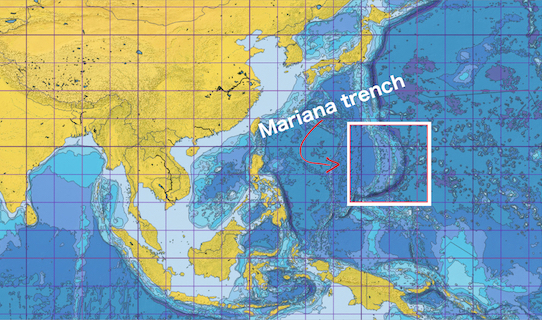
\includegraphics[width=6cm]{Fig-1.jpg}.
		\caption{Mariana Trench: square of the study area}
\end{figure}
\end{frame}

\subsection{Geology}

\begin{frame}\frametitle{Mariana Trench:\\Geological characteristics}
	\begin{exampleblock}{Bathymetry}
- transverse profile is strongly asymmetric: the slopes are higher on the side of the island arc. The slopes are dissected by deep underwater canyons. Various narrow steps are often found on the slopes of the trench.
	\end{exampleblock}
	\begin{exampleblock}{Geomorphology}
- complicated steps of various shapes and sizes, caused by active tectonic and sedimental processes. Hence, it is the largest structural trap located in the continental margins of the Pacific Ocean.
	\end{exampleblock}
	\begin{alertblock}{Sediments}
- the sediments are being carrying by the ocean waves in a clockwise direction, passing through the trenches on the west of the Pacific, i.e. the Kermadec Trench, Tonga Trench, Samoan Passage.
	\end{alertblock}
\end{frame}

\begin{frame}\frametitle{Map of the Mariana Trench}
	\begin{figure}[H]
			\centering
		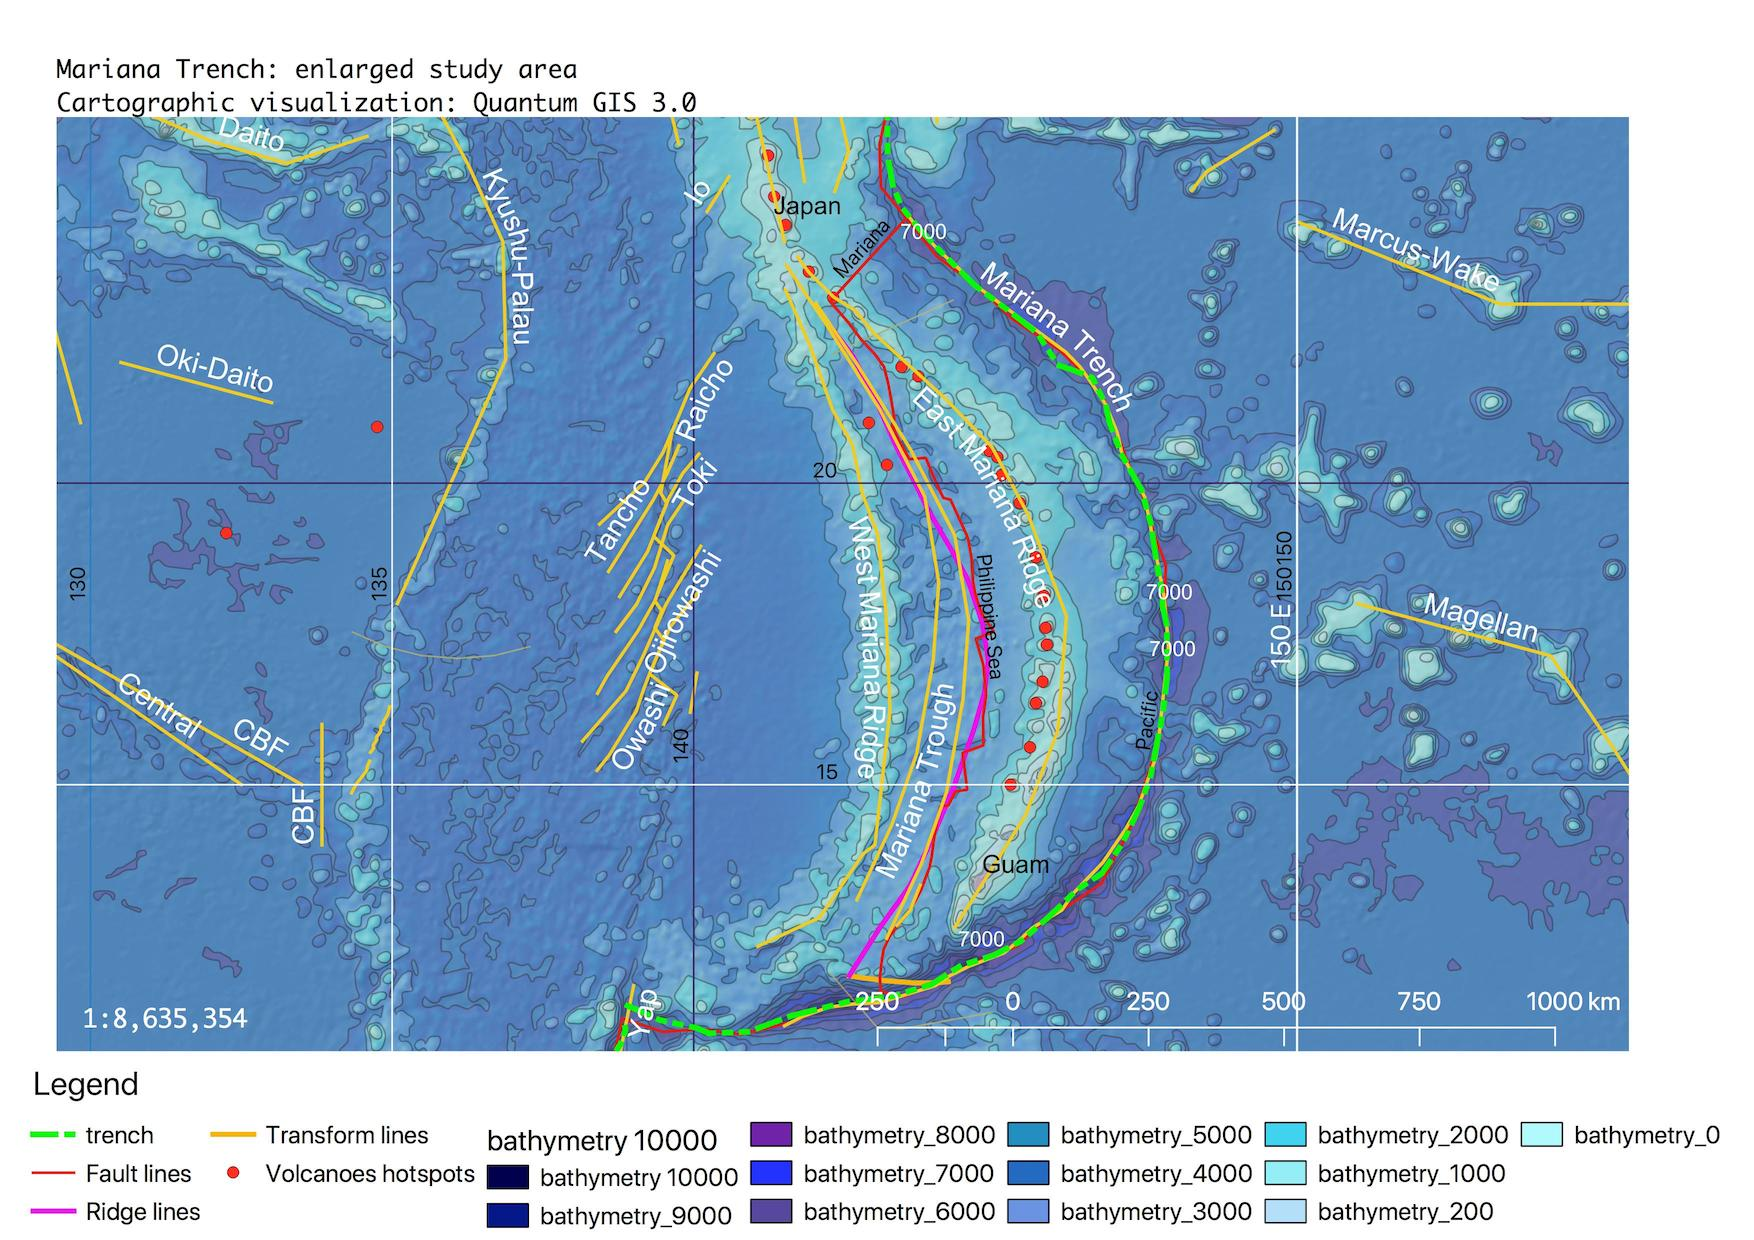
\includegraphics[width=9cm]{Fig-2.jpg}.\caption{Enlarged map of the Mariana Trench}
	\end{figure}
\end{frame}
\subsection{Tectonics}

\begin{frame}\frametitle{Tectonics - I}
\begin{itemize}
    \item<1-> Mariana Trench crosses four tectonic plates: Mariana, Caroline, Pacific and Philippine. 
    \item<2-> The formation of the Mariana Trench is caused by complex and diverse geomorphic factors. 
    \item<3-> Mariana Trench presents a complex system with highly interconnected factors: 
    	 \begin{itemize}
            	\item geology (sediment thickness across 4 tectonic plates), 
            	\item bathymetry (coordinates, depth values in the observation points), 
           	 \item geometry of the slopes: angle and steepness, 
           	 \item oceanography (deep sea currents), 
           	 \item volcanology,
            	\item deep sea marine biology. 
           \end{itemize}
\end{itemize}
\end{frame}

\begin{frame}\frametitle{Tectonics - II}
The system of the Mariana trench is complicated and consists of the interrelated factors forming its tectonic structure:
 \begin{itemize}
            \item The main part of the seabed of the Mariana Trench is composed by the oceanic crust forming rift zones of the mid-ocean ridges with a capacity of 5 to 10 km (Morgan, 1974). 
            \item The deformations of the trench respond to the coupling between the upper and lower plates relating to the continental slab age-buoyancy (Ruff \& Kanamori, 1980) ,
            \item The back-arc deformation roughly correlate with upper continental tectonic plate velocity (Heuret \& Lallemand, 2005). 
            \item The trench migration rates are chiefly controlled by the lower continental tectonic plate velocity (Lallemand et al, 2008), 
            \item In turn, tectonic plate velocity depends on the tectonic slab age buoyancy (Chase, 1978).
\end{itemize}
\end{frame}

\subsection{Technical Approach}
\begin{frame}\frametitle{Technical Approach}
To study such a complex system as Mariana Trench, an objective method combining various approaches (statistics, R, GIS, descriptive analysis and graphical plotting) was performed. \\Thus, the methodology includes following steps:
\begin{itemize}
    \item<1-> Data capture in GIS, vector thematic data were processed in QGIS: tectonics, bathymetry, geomorphology and geology.
    \item<2-> Programming on R language
      \begin{itemize}
            \item statistics
            \item descriptive analysis 
            \item graphical plotting  
        \end{itemize}
      \item<3-> Geospatial comparative analysis of variables by 4 tectonic plates
\end{itemize}
\end{frame}

% ----------------------------------------------------------------------------
% *** END of Introduction >>>
% ----------------------------------------------------------------------------

% ----------------------------------------------------------------------------
% *** START: Methodology <<<
% ----------------------------------------------------------------------------
\section{Methodology}
\subsection{Workflow}
\begin{frame}
\frametitle{Methodology (Brief)}
The methodology includes following steps. 
\begin{itemize}
    \item<1-> firstly, vector thematic data were processed in QGIS: tectonics, bathymetry, geomorphology and geology.
    \item<2-> secondly, 25 cross-section profiles were drawn across the trench. The length of each profile is 1000-km. 
        \begin{itemize}
            \item the attribute information has been derived from each profile and stored in a table containing coordinates, depths and thematic information.
            \item this table was processed by methods of the statistical analysis on R
        \end{itemize}
      \item<3-> thirdly, performed geospatial comparative analysis to estimate effects of the data distribution by 4 tectonic plates: slope angle, igneous volcanic areas and depths.
\end{itemize}
\end{frame}
% ----------------------------------------------------------------------------
% *** END: Methodology >>>
% ----------------------------------------------------------------------------

% ----------------------------------------------------------------------------
% *** START: Data <<<
% ----------------------------------------------------------------------------
\section{GIS Project}
\subsection{GIS digitizing}
\begin{frame}
\frametitle{Data Capture in GIS}
			
The GIS part of the research is performed in the QGIS 3.0. 
Geospatial tasks by QGIS plugins: reading coordinates, crossing profile lines, reading data from attribute table into .csv format. Various geospatial data have been uploaded into the GIS project: bathymetry (depths), sediment thickness, location of igneous volcanic zones, tectonic plates, etc. The GIS project: UTM cartesian coordinate system (square N-55). 
\begin{figure}[H]
	\centering
		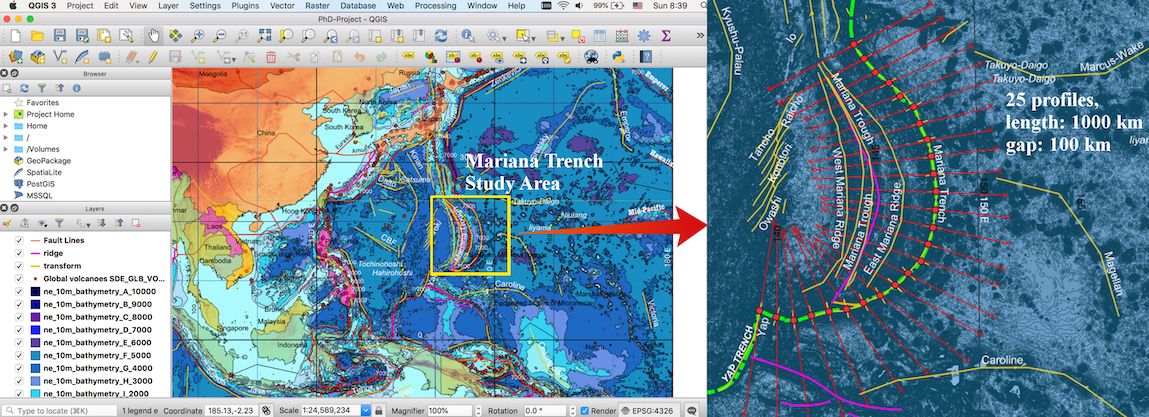
\includegraphics[width=8cm]{Fig-2-1.jpg}
	\caption{Digitizing 25 bathymetric profiles across the Mariana Trench}\label{fig:2-1}
\end{figure}		
\end{frame}
% ----------------------------------------------------------------------------
% *** END: Data >>>
% ----------------------------------------------------------------------------

% ----------------------------------------------------------------------------
% *** START: Workflow <<<
% ----------------------------------------------------------------------------
\subsection{GIS Workflow}
\begin{frame}
\frametitle{Digitizing bathymetric profiles}

\begin{figure}[H]
	\centering
		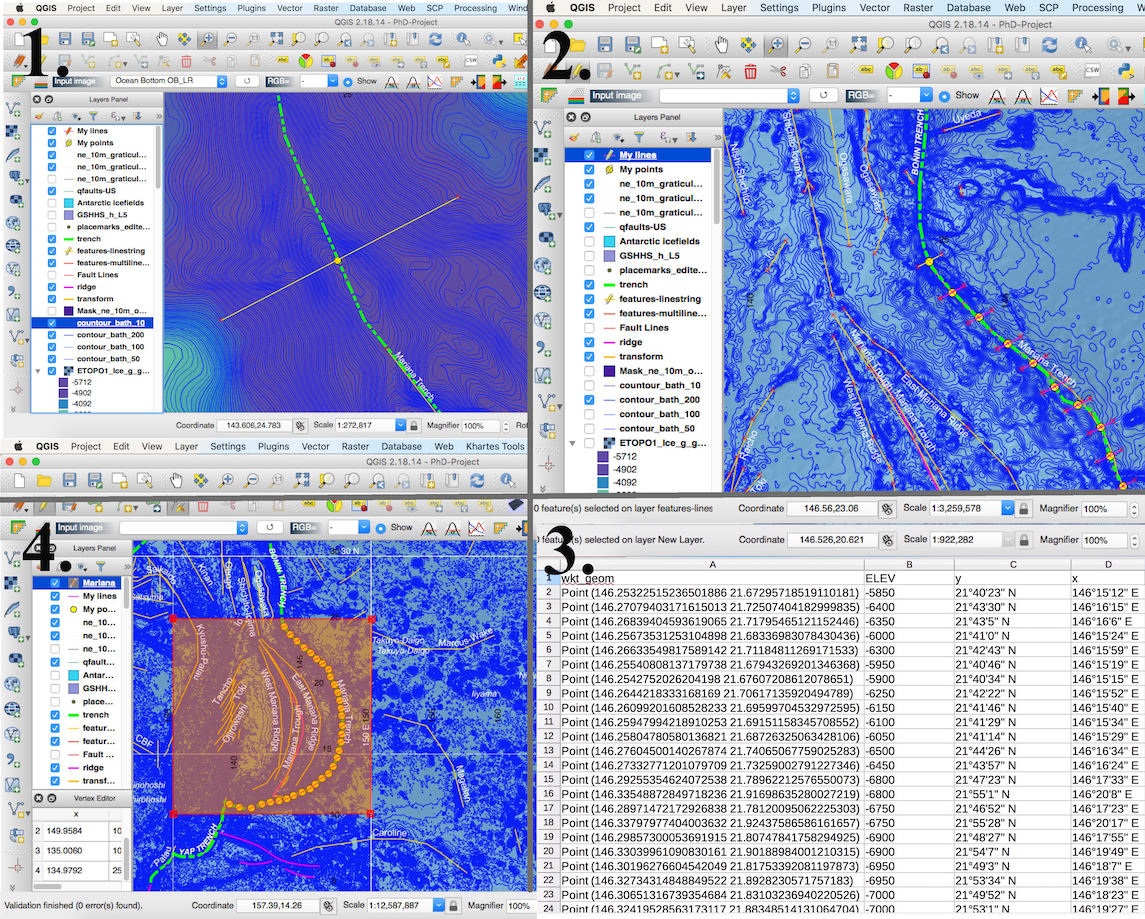
\includegraphics[width=8cm]{Fig-2-2.jpg}
	\caption{Digitizing 25 bathymetric profiles across the Mariana Trench}\label{fig:2-2}
\end{figure}		
\end{frame}

\subsection{\LaTeX \space Plotting}

\begin{frame}[fragile]\frametitle{\TeX \space macro language code for \\bathymetric plotting. Example for profile 16, 17, 18.}
\begin{Verbatim}[fontsize=\scriptsize]
\begin{filecontents*}{MyTab18.csv}
ELEV ,y2,x2
145.528246366,47.0433461696,-7800 # bathymetric data here in 3 columns 
\end{filecontents*}
\begin{tikzpicture}
\begin{axis}[grid=major,minor x tick num=10,minor y tick num=10,
	colorbar sampled line,colormap name=bluered,
	title={Mariana Trench. Bathymetric Profiles Nr.16,17,18},
	ylabel={Depth (m)},
	legend entries={Profile18,Profile17,Profile16,},
	scaled ticks=false,
	yticklabel style={/pgf/number format/fixed,/pgf/number format/fixed zerofill,}]
\addplot+ [scatter,only marks,mark=Mercedes star flipped,colormap name=bluered,]
table [x=x, y=d, col sep=comma] {MyTab16.csv};
\addplot+ [scatter, colorbar sampled line,only marks,mark=asterisk,colormap
name=bluered,] 
table [x=long, y=d, col sep=comma] {MyTab17.csv};
\addplot+ [scatter, colorbar sampled line,only marks,mark=10-pointed star,colormap
name=bluered,] 
table [x=y2,y=ELEV, col sep=comma] {MyTab18.csv}; 
\end{axis} 
\end{tikzpicture}
\end{Verbatim}
\end{frame}

\begin{frame}\frametitle{\LaTeX \space for bathymetry}
\frametitle{\LaTeX \space for bathymetry}

\begin{figure}[H]
	\centering
		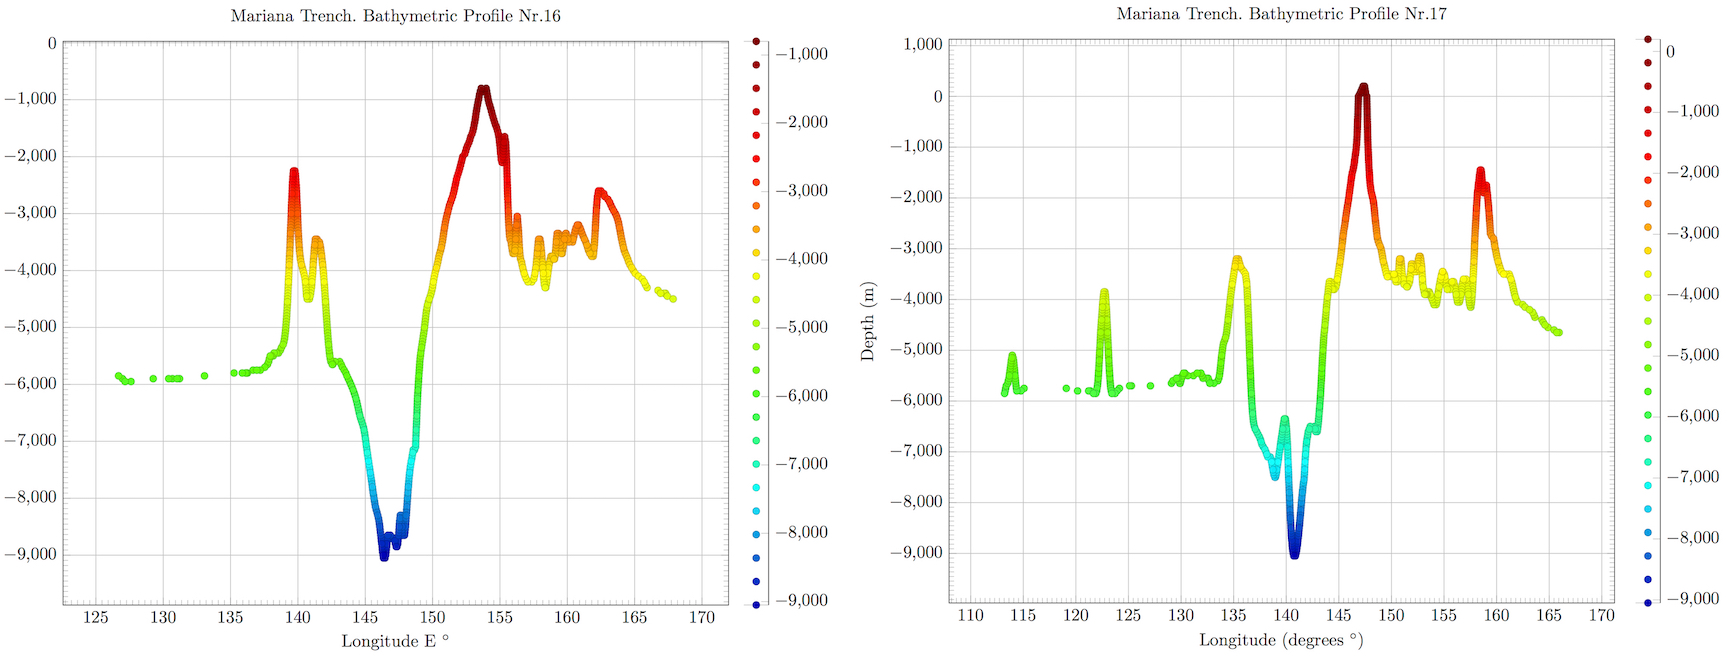
\includegraphics[width=11cm]{Fig-2-3.jpg}
	\caption{\LaTeX \space Plotting: two selected profiles, 2D View}\label{fig:2-3}
\end{figure}		
\end{frame}

\begin{frame}\frametitle{\LaTeX \space for bathymetry:\\3D plotting}
\begin{figure}[H]
	\centering
		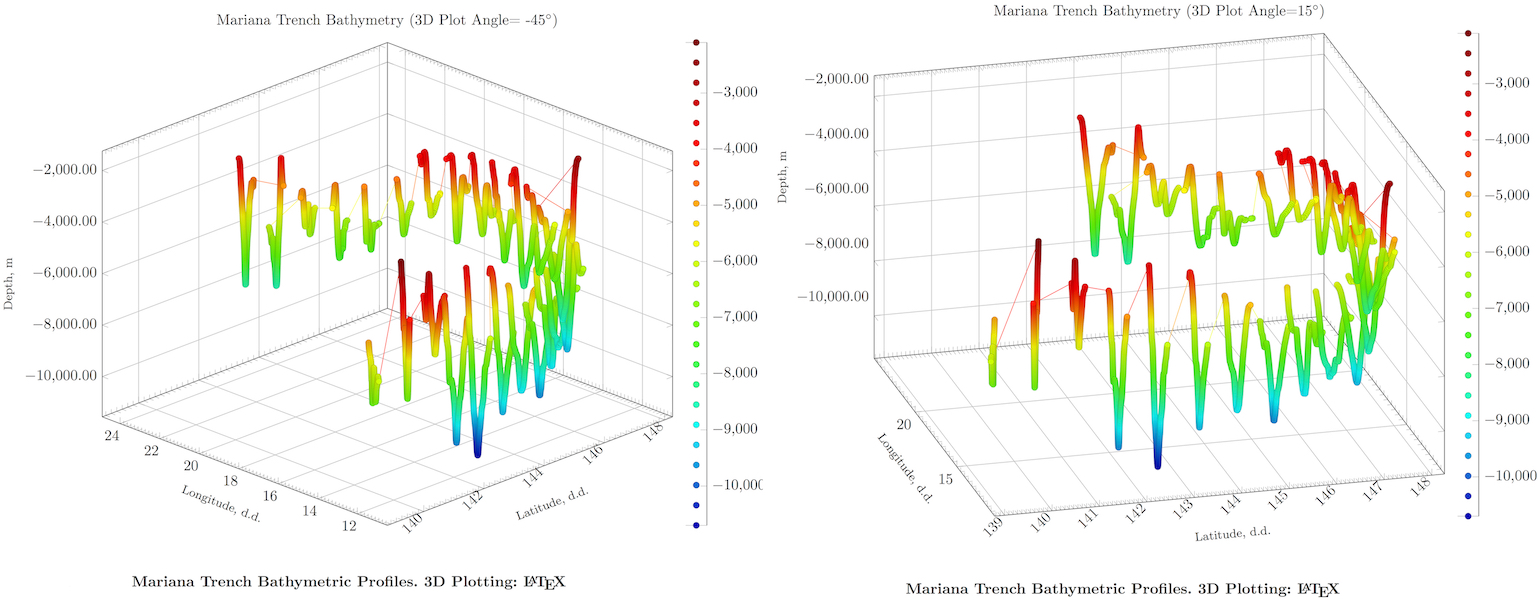
\includegraphics[width=11cm]{Fig-2-4.jpg}
	\caption{\LaTeX \space Plotting: Marina Arc, 3D View}\label{fig:2-4}
\end{figure}		
\end{frame}

\section{Statistical Analysis by R}
\subsection{Data Distribution}
\begin{frame}\frametitle{Graph:\\bathymetric profiles}
\begin{figure}[H]
	\centering
		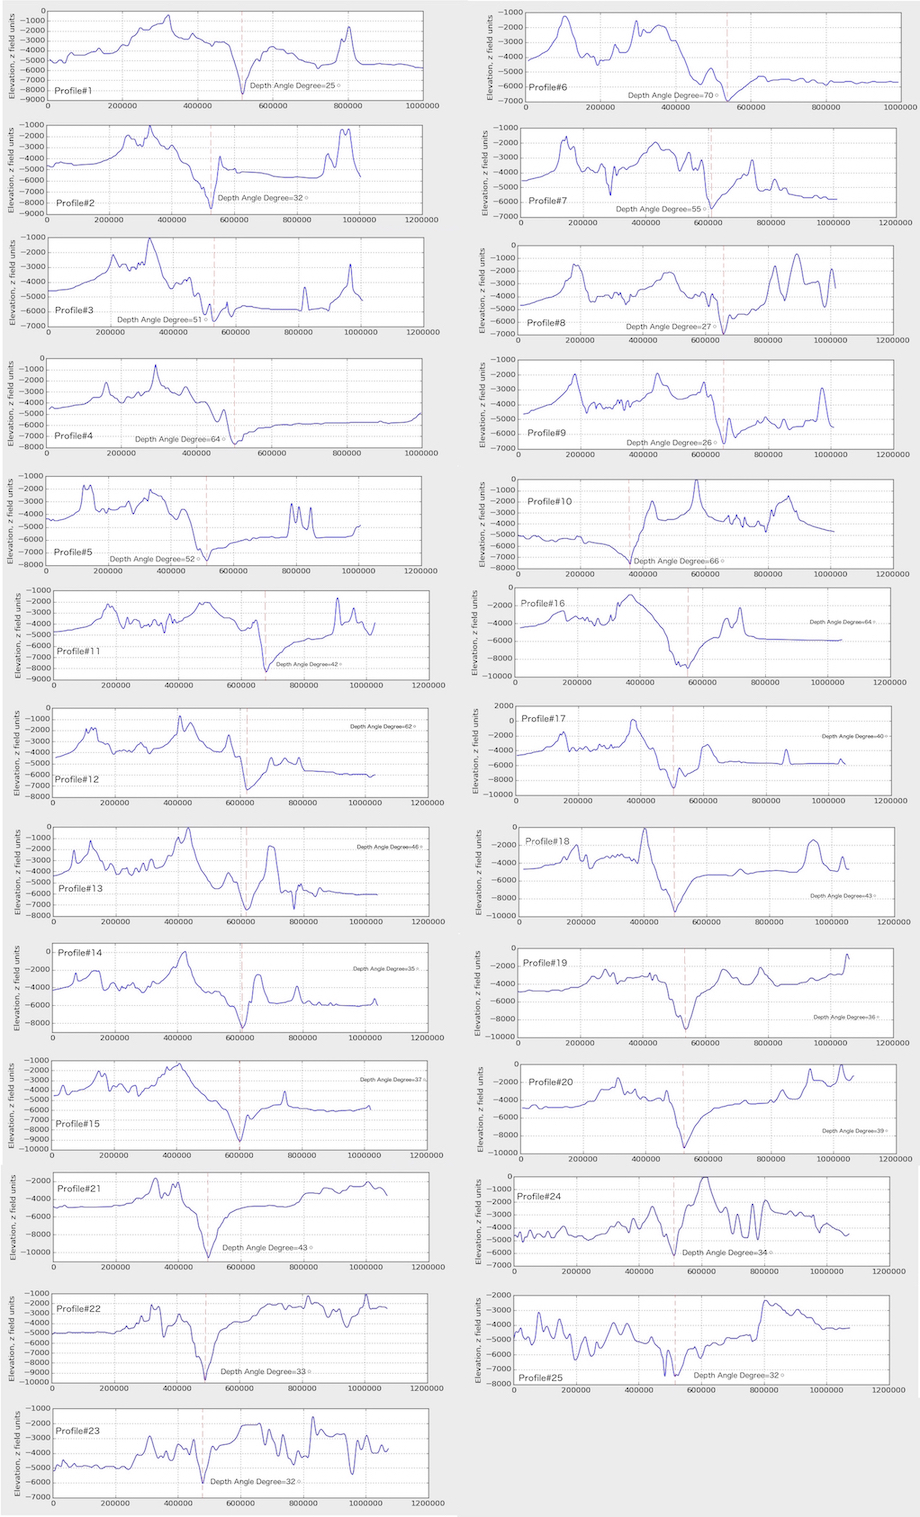
\includegraphics[width=4cm]{Fig-2-5.jpg}
	\caption{Graphs of the 25 bathymetric profiles, Mariana Trench}\label{fig:2-5}
\end{figure}		
\end{frame}

\begin{frame}[fragile]\frametitle{R code to generate boxplots 'whiskerplots' using default boxplot function}
\begin{lstlisting}[language=R]
#BoxPlot (or WhiskerPlot)
# Part 1: create data.frame
	# step-1. read-in table. generate data frame.
MDepths <- read.csv("Depths.csv", header=TRUE, sep = ",")
	# step-2. clean up data frame from NA values
MDepths <- na.omit(MDepths) 
row.has.na <- apply(MDF, 1, function(x){any(is.na(x))}) # check up deleted NA
sum(row.has.na) # sum up NA values: [1] 0
head(MDepths) # look up cleaned data frame.

# Part 2: create "whisker boxplot"
	# step-3. generate list of profiles (to be shon on axis X)
profile_names <- paste(c("profile"), seq(1:25), sep="") 
	# step-4. generate box plot using arguments (here: 25 profiles)
p<- boxplot(MDepths$profile1, MDepths$profile2, MDepths$profile3, MDepths$profile4, MDepths$profile5, MDepths$profile6,MDepths$profile7, MDepths$profile8, MDepths$profile9, MDepths$profile10, MDepths$profile11, MDepths$profile12, MDepths$profile13, MDepths$profile14, MDepths$profile15, MDepths$profile16, MDepths$profile17, MDepths$profile18, MDepths$profile19, MDepths$profile20, MDepths$profile21, MDepths$profile22, MDepths$profile23, MDepths$profile24, MDepths$profile25,     
	main = "Mariana Trench Depths Boxplot", 
	outline = TRUE,
	outlier.color = "seagreen", outlier.shape = 8, outlier.size = 2,    
#	xlab = "Profiles",         
	ylab = "Depths",         
	las = 2,         
	col = viridis(25, alpha=.2),         
	names = profile_names)
p
\end{lstlisting}
\end{frame}

\begin{frame}\frametitle{Statistical Boxplots}
\begin{figure}[H]
	\centering
		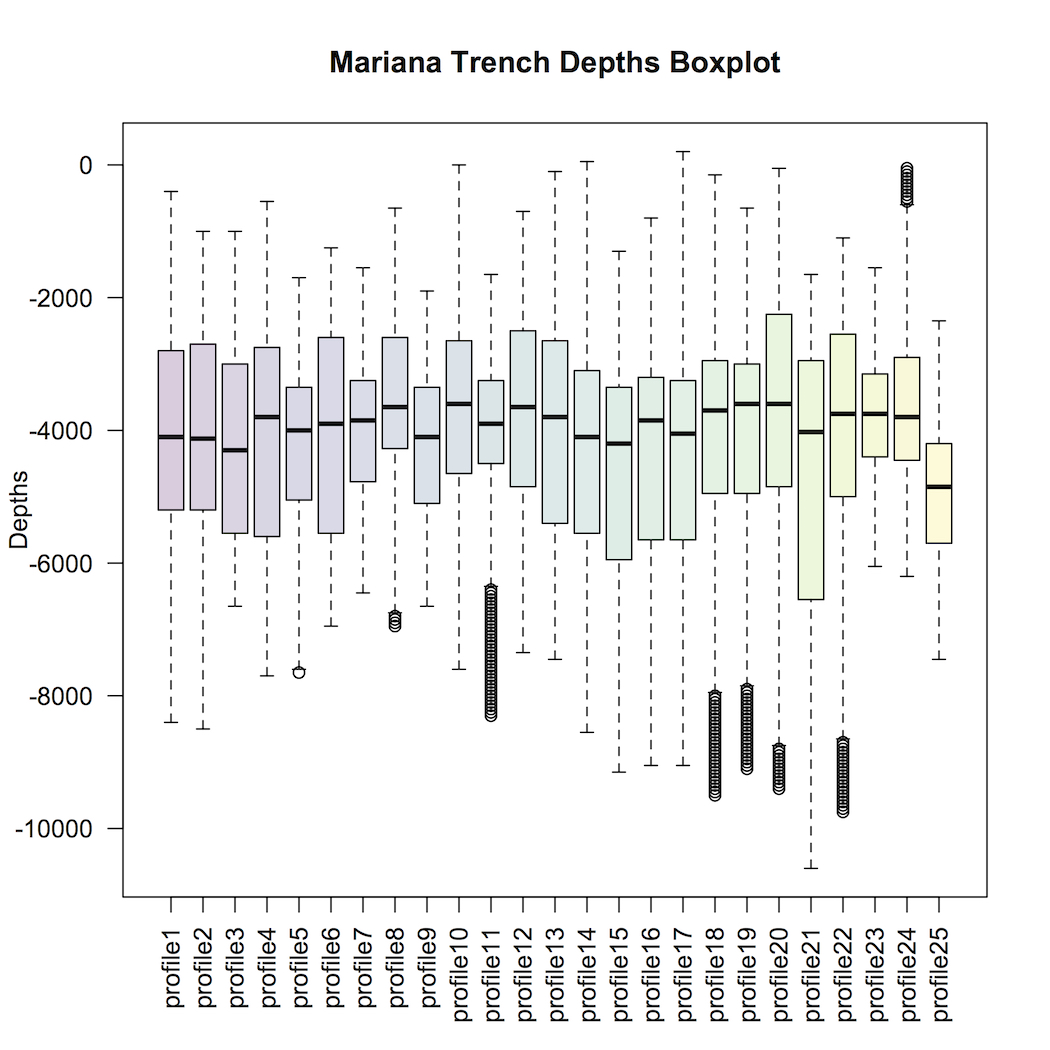
\includegraphics[width=6cm]{Fig-2-6.jpg}
	\caption{Statistical box plots}
\end{figure}		
\end{frame}

\begin{frame}\frametitle{'Violin' Plots}
The violin plots show Kernel probability density distribution of the bathymetric observations, as multimodal distributions with multiple peaks. Kernel density distribution plot was created using library \{violinmplot\} of R in a combined plot, which includes calculated quantiles for 0.25 and 0.75 of the data pool. 
\begin{figure}[H]
	\centering
		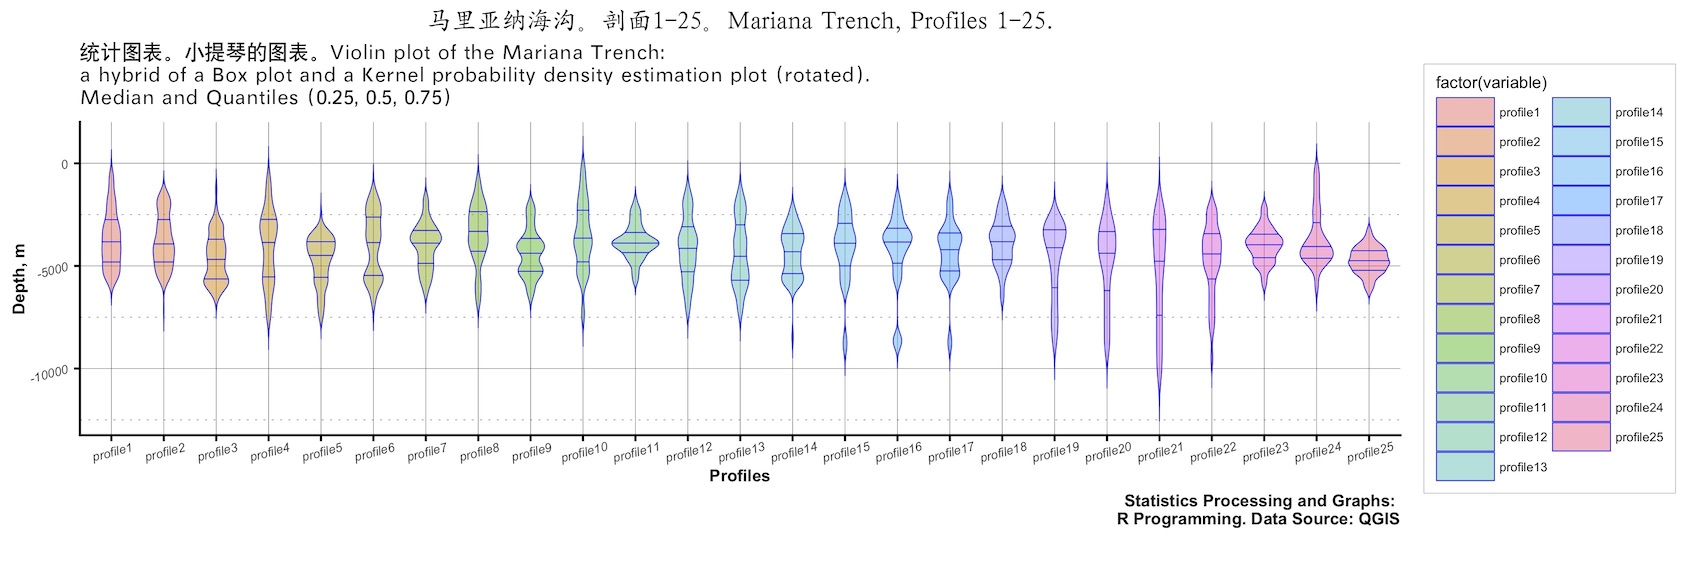
\includegraphics[width=11cm]{Fig-2-7.jpg}\caption{Visualization of the 'Violin' plots for 25 bathymetric profiles}
\end{figure}		
\end{frame}

\begin{frame}[fragile]\frametitle{R code for 'violin' plots using \{violinmplot\} library: statistical analysis of data distribution: steps 1-4}
\begin{lstlisting}[language=R]
# Part-1. Prepare data frame
	# step-1. read in table with data. create initial data frame. clean data frame from the NA
MDepths <- read.csv("Depths.csv", header=TRUE, sep = ",")
Ml <- na.omit(MDepths) 
row.has.na <- apply(Ml, 1, function(x){any(is.na(x))}) 
sum(row.has.na) 
head(Ml)
	# step-2. Merge columns with identical attributes
MDTt = melt(setDT(Ml), measure = patterns("^profile"), value.name = c("depth"))
head(MDTt)
# Part-2. Plot 'violin plot' - statistical analysis of bathymetric data distribution (mean, standard deviation, median).
	# step-3. variant-1. via library(violinmplot) 	
library(violinmplot) 
violinmplot(depth ~ variable, MDTt, horizontal=FALSE, col.violin = "blue", main = "Violin plot of the Mariana Trench: a hybrid of a Box plot and a Kernel probability density estimation plot (rotated) + median")
	# step-4.  variant-2. via library(ggplot2) 	
g<- ggplot(MDTt, aes(variable, depth)) +    
	geom_violin(aes(fill = factor(variable)), colour = "blue", size = 0.2, draw_quantiles = c(0.25, 0.5, 0.75), alpha = 0.5, scale = "count", trim = FALSE)
g
\end{lstlisting}
\end{frame}

\begin{frame}[fragile,shrink=20]\frametitle{R code for 'violin' plots using \{violinmplot\} library: statistical analysis of data distribution: step 5.}
\begin{lstlisting}[language=R]
	# step-5. add title, axises, etc.
Violin<- g +
	xlab("Profiles") + 
	ylab("Depth, m") +
	labs(
	title = "Mariana Trench, Profiles 1-25.", 
	subtitle = "Violin plot of the Mariana Trench: \na hybrid of a Box plot and a Kernel probability density estimation plot (rotated). \nMedian and Quantiles (0.25, 0.5, 0.75)",
	caption = "Statistics Processing and Graphs: \nR Programming. Data Source: QGIS") +
	theme(plot.margin = margin(5, 10, 20, 5),
		plot.title = element_text(family = "Kai", face = "bold", size = 12),
		plot.subtitle = element_text(family = "Hei", face = "bold", size = 10),
		plot.caption = element_text(face = 2, size = 8),
		panel.background=ggplot2::element_rect(fill = "white"),
		legend.justification = "right", legend.position = "right",
		legend.box.just = "right", legend.direction = "vertical",
		legend.box = "vertical", legend.box.background = element_rect(colour = "honeydew4",size=0.2),
		legend.background = element_rect(fill = "white"),
		legend.key.width = unit(1,"cm"),legend.key.height = unit(.5,"cm"),
		legend.spacing.x = unit(.2,"cm"),legend.spacing.y = unit(.1,"cm"),
		legend.text = element_text(colour="black", size=6, face=1),
		legend.title = element_text(colour="black", size=8, face=1),
		strip.text.x = element_text(colour = "white", size=6, face=1),
		panel.grid.major = element_line("gray24", size = 0.1, linetype = "solid"),
		panel.grid.minor = element_line("gray24", size = 0.1, linetype = "dotted"),
		axis.text.x = element_text(face = 3, color = "gray24", size = 6, angle = 15),
		axis.text.y = element_text(face = 3, color = "gray24", size = 6, angle = 15),
		axis.ticks.length=unit(.1,"cm"),axis.line = element_line(size = .3, colour = "grey80"),
		axis.title.y = element_text(margin = margin(t = 20, r = .3), face = 2, size = 8),
		axis.title.x = element_text(face = 2, size = 8, margin = margin(t = .2))) +
		guides(col = guide_legend(nrow = 13, ncol = 2, byrow = TRUE)) # improve design
Violin		
\end{lstlisting}
\end{frame}

\begin{frame}\frametitle{Regression Analysis:\\Bathymetric Profiles}
\begin{figure}[H]
	\centering
		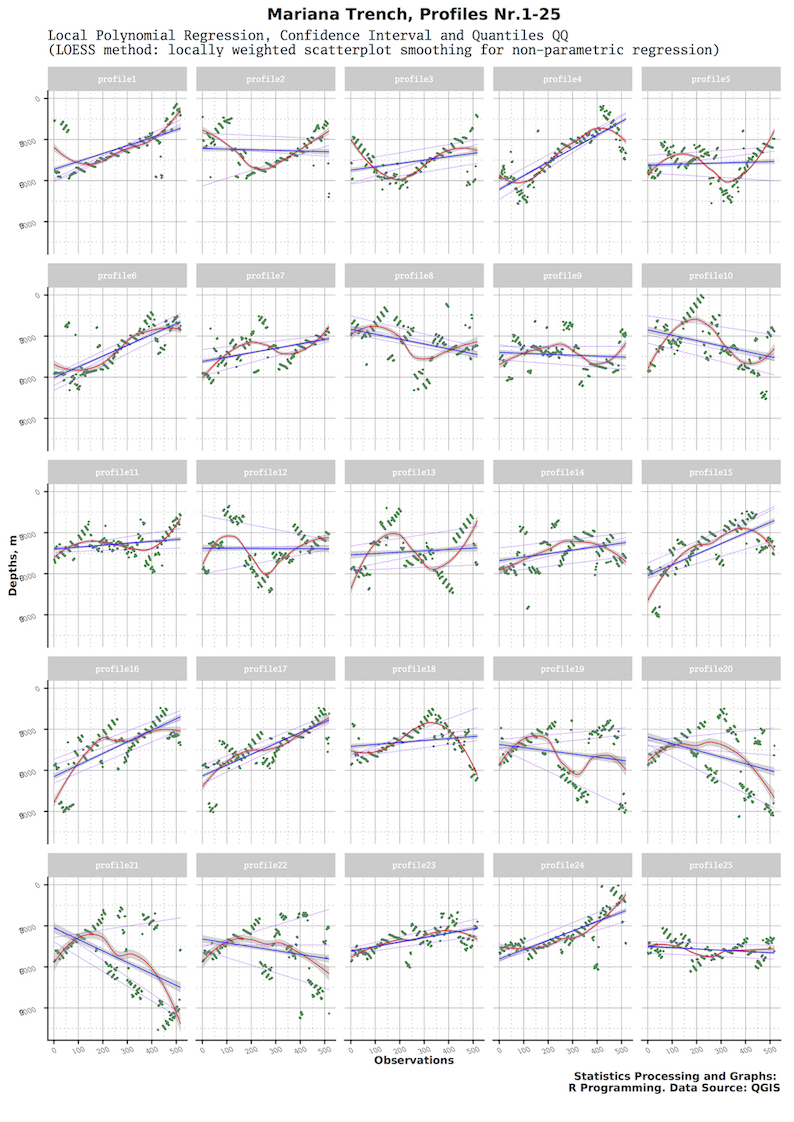
\includegraphics[width=4.5cm]{Fig-2-8a.jpg}
	\caption{Regression Analysis: 25 profiles}
\end{figure}		
\end{frame}

\begin{frame}[fragile,shrink=10]\frametitle{R code for regression analysis, bathymetric profiles.\\ Parts 1 and 2: data.frame, parameters}
\begin{lstlisting}[language=R]
# Part 1: create data.frame
	# step-1. read in table, create data frame.
MDepths <- read.csv("Depths.csv", header=TRUE, sep = ",")
	# step-2. clean up data frame from the NA
MDF <- na.omit(MDepths) 
row.has.na <- apply(MDF, 1, function(x){any(is.na(x))}) 
(row.has.na) # sum up NA, result: [1] 0
head(MDF) #  
# Part 2: perform regression analysis and plot (Mathematical method includes 3 types of curves with confidence intervals and quantiles).
	# step-3. (here: profile \#11) 
Loess_profile11 <- ggplot(MDF, aes(x = observ, y = profile11)) +
	geom_point(aes(x = observ, y = profile11, colour = "Samples", shape = "Samples"), show.legend=TRUE) +
	geom_smooth(aes(x = observ, y = profile11, colour = "Loess method"), method = loess, se = TRUE, span = .4, size=.3, linetype = "solid", show.legend=TRUE) +
	geom_smooth(aes(x = observ, y = profile11, colour = "Glm method"), method = glm, se = FALSE, span = .4, size=.4, linetype = "dotted", show.legend=TRUE) +
	geom_smooth(aes(x = observ, y = profile11, colour = "Lm method"), method = lm, se = TRUE, size=.3, linetype = "solid", show.legend=TRUE) +
	geom_quantile(aes(x = observ, y = profile11, colour = "Quantiles"), linetype = "solid", show.legend=TRUE) +
	xlab("Observations") +  ylab("Depths, m") +
	scale_color_manual(values = c("Samples" = "seagreen", "Loess method" = "red", "Lm method" = "blue", "Glm method" = "orange", "Quantiles" = "purple")) + # set up colors
	scale_shape_manual(values = c("Samples" = 1)) + # set up shapes (here: \#1 - "transparent circle")
	labs(title="Mariana Trench, Profile 11.", 
	subtitle = "Local Polynomial Regression, \nConfidence Interval, Quantiles \n(LOESS method: locally weighted scatterplot \nsmoothing for non-parametric regression)",
	caption = "Statistics Processing and Graphs: \nR Programming. Data Source: QGIS") + theme(
	\end{lstlisting}
\end{frame}

\begin{frame}[fragile,shrink=10]\frametitle{R code for regression analysis, bathymetric profiles.\\ Part 2: theme, layout}
\begin{lstlisting}[language=R]
	theme(plot.margin = margin(5, 10, 20, 5),
		plot.title = element_text(family = "Kai", face = "bold", size = 8),
		plot.subtitle = element_text(family = "Hei", face = "bold", size = 6),
		plot.caption = element_text(face = 2, size = 6),panel.background=ggplot2::element_rect(fill = "white")
		legend.justification = "bottom", legend.position = "bottom",legend.box.just = "right",
		legend.direction = "horizontal",legend.box = "horizontal",
		legend.box.background = element_rect(colour = "honeydew4",size=0.2),
		legend.background = element_rect(fill = "white"),
		legend.key.width = unit(1,"cm"),legend.key.height = unit(.5,"cm"),
		legend.spacing.x = unit(.2,"cm"),legend.spacing.y = unit(.1,"cm"),
		legend.text = element_text(colour="black", size=6, face=1),
		legend.title = element_text(colour="black", size=6, face=1),
		strip.text.x = element_text(colour = "white", size=6, face=1),
		panel.grid.major = element_line("gray24", size = 0.1, linetype = "solid"),
		panel.grid.minor = element_line("gray24", size = 0.1, linetype = "dotted"),
		axis.text.x = element_text(face = 3, color = "gray24", size = 6, angle = 15),
		axis.text.y = element_text(face = 3, color = "gray24", size = 6, angle = 15),
		axis.ticks.length=unit(.1,"cm"),axis.line = element_line(size = .3, colour = "grey80"),
		axis.title.y = element_text(margin = margin(t = 20, r = .3), face = 2, size = 8),
		axis.title.x = element_text(face = 2, size = 8, margin = margin(t = .2))) +
		guides(col = guide_legend(nrow = 1, ncol = 6, byrow = TRUE)) 
Loess_profile11
# Part 2: combine 3 plots on one layout
library(ggpubr)
#ggarrange function
Regression_Profiles111824 <- ggarrange(Loess_profile11, Loess_profile18, Loess_profile24, labels = c("1", "2", "3"), ncol = 3, nrow = 1, common.legend = TRUE, legend = "bottom")
\end{lstlisting}
\end{frame}
	
\begin{frame}\frametitle{Regression Analysis:\\Enlarged Selected Profiles}
\begin{figure}[H]
	\centering
		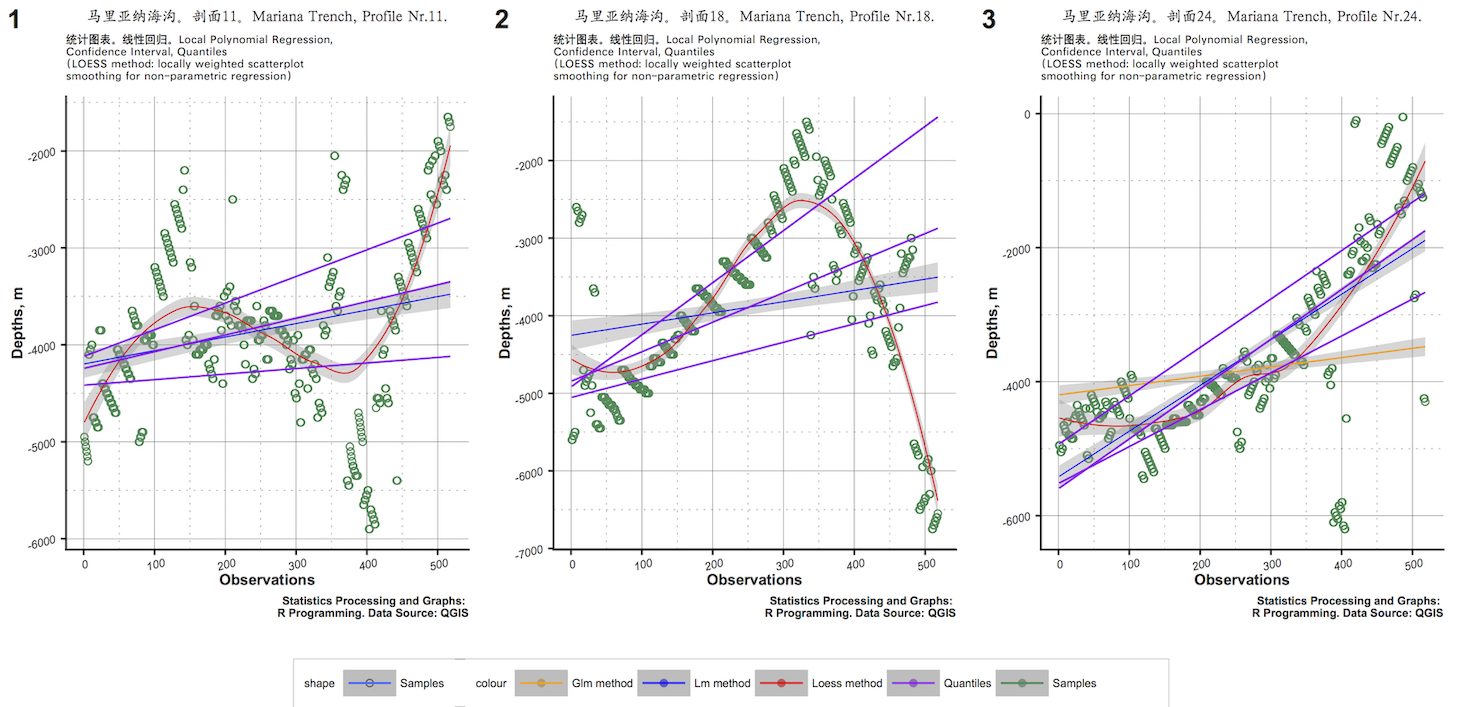
\includegraphics[width=11cm]{Fig-2-8b.jpg}
	\caption{Regression Analysis: 3 selected profiles}
\end{figure}		
\end{frame}

\begin{frame}\frametitle{Statistical Histograms}
\begin{figure}[H]
	\centering
		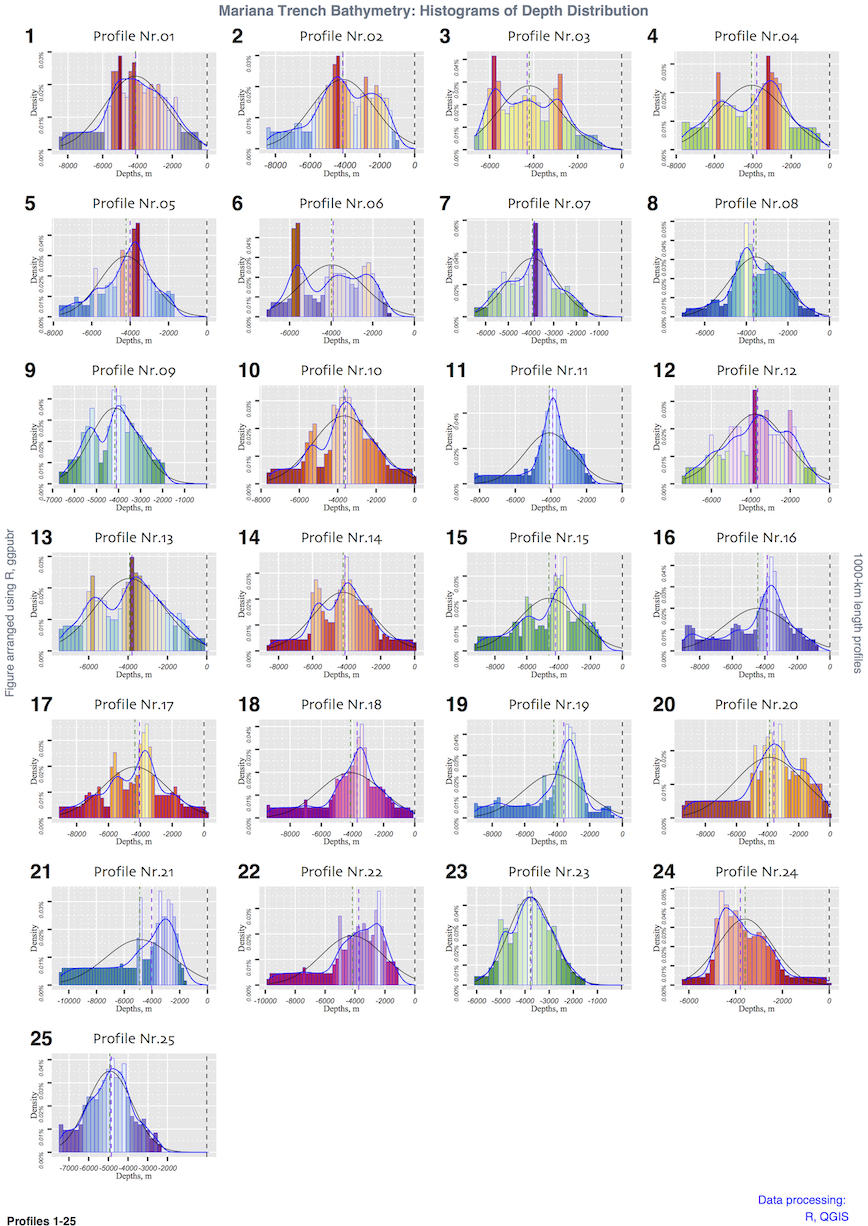
\includegraphics[width=4cm]{Fig-2-9.jpg}\caption{Visualized multi-plot for statistical histograms, Mariana Trench}
\end{figure}		
\end{frame}

\begin{frame}[fragile,shrink=20]\frametitle{R code to create histograms using \{ggplot\} library}
\begin{lstlisting}[language=R]
MDepths <- read.csv("Depths.csv", header=TRUE)
X01<- MDepths[,01]
X01<-X01[!is.na(X01)]
as.data.frame(X01)
dat01<- data.frame(X01)
p01<-ggplot(dat01, aes(X01)) + labs(title = "Profile Nr.01", x = "Depths, m", y = "Density") +
theme(plot.title = element_text(family = "Skia", face=2, size=10),panel.background=ggplot2::element_rect(fill = "gray91"),
legend.position = c(.95, .95), legend.justification = c("right", "top"),  legend.box.just = "right",
legend.margin = margin(6, 6, 6, 6), legend.direction = "vertical", 
legend.background = element_blank(),legend.key.width = unit(.5,"cm"),legend.key.height = unit(.3,"cm"),
legend.spacing = unit(.3,"cm"), legend.box.background = element_rect(colour = "honeydew4",size=0.2),
legend.text = element_text(family = "Arial", colour="black", size=6, face=1),
legend.title = element_blank(),strip.text.x = element_text(colour = "white"),
panel.grid.major = element_line("white", size = 0.3),
panel.grid.minor = element_line("white", size = 0.3, linetype = "dotted"),
axis.text.x = element_text(family = "Arial", face = 3, color = "gray24",size = 5, angle = 0),
axis.text.y = element_text(family = "Arial", face = 3, color = "gray24",size = 4, angle = 90),
axis.ticks.length=unit(.1,"cm"), axis.line = element_blank(),
axis.title.y = element_text(margin = margin(t = 20, r = .3), family = "Times New Roman", face = 1, size = 6),
axis.title.x = element_text(family = "Times New Roman", face = 1, size = 6,margin = margin(t = .2))) +
scale_x_continuous(breaks=pretty(dat01$X01, n=4), minor_breaks=seq(min(dat01$X01), max(dat01$X01), by=500)) +
scale_y_continuous(breaks = scales::pretty_breaks(n = 4),labels = scales :: percent) +
scale_fill_distiller(palette = "RdGy") +
scale_color_manual(name = "Statistics:", values = c(median = "purple", mean = "green4",density = "blue", norm_dist = "black")) +
geom_histogram(binwidth = 200,aes(fill = ..density..,x = dat01$X01,y = ..density..),color = "blue",size = .1) +
stat_function(fun = dnorm, args = list(mean = mean(dat01$X01), sd = sd(dat01$X01)), lwd = 0.2, color = 'black') +
stat_density(geom = "line", size = .3, aes(color = "density")) +
geom_vline(aes(color = "mean", xintercept = mean(X01)), lty = 4, size = .3) +
geom_vline(aes(color = "median", xintercept = median(X01)), lty = 2, size = .3)  +
geom_vline(aes(color = "norm_dist", xintercept = dnorm(X01)), lty = 2, size = .3)
p01
\end{lstlisting}
\end{frame}

\begin{frame}\frametitle{Ridgeline Plots}
\begin{figure}[H]
	\centering
		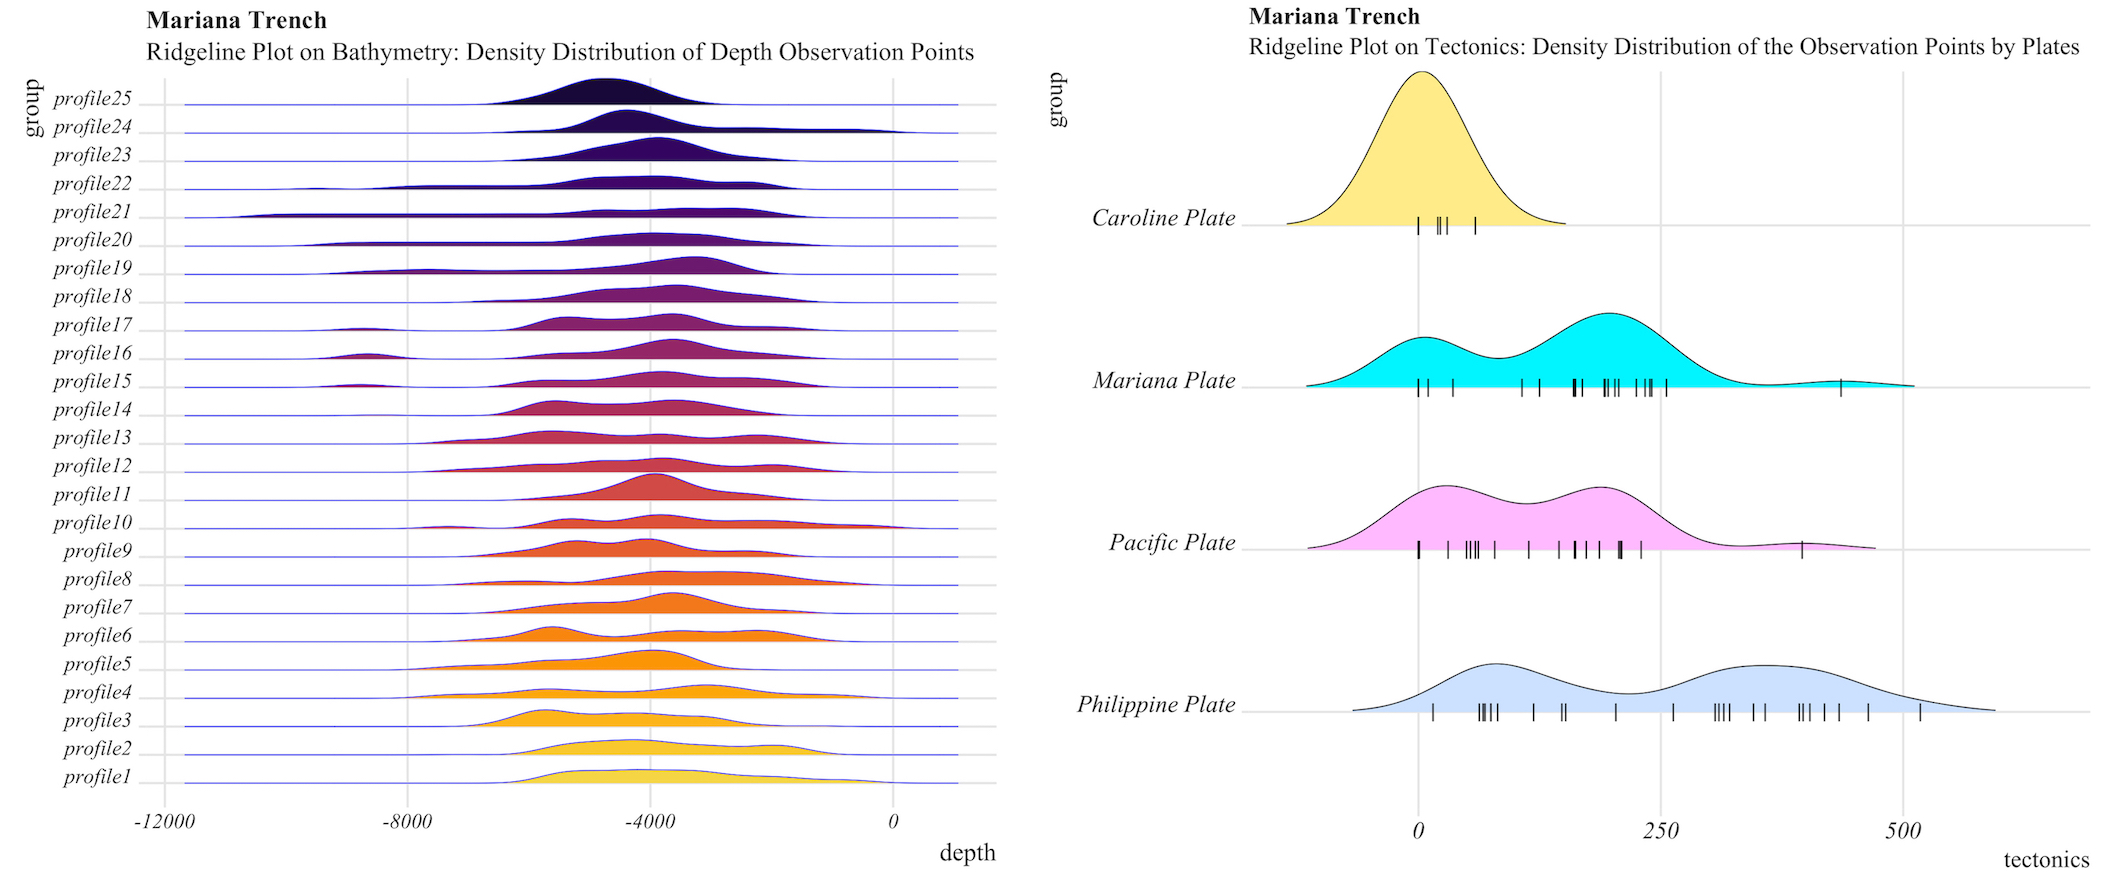
\includegraphics[width=11cm]{Fig-2-10.jpg}
	\caption{R: visualization of the ridgeline plots.}
\end{figure}		
\end{frame}

\begin{frame}[fragile,shrink=20]\frametitle{R code for ridgeline plots by\\ \{ggridges\} and \{ggplot2\} libraries: Part 1}
\begin{lstlisting}[language=R]
library(ggridges)
library(ggplot2)
# Part-1 for tectonic plates
	# step-1. Read in table, create data frame 
MDF <- read.csv("Morphology.csv", header=TRUE, sep = ",")
MDF <- na.omit(MDF) 
row.has.na <- apply(MDF, 1, function(x){any(is.na(x))}) 
sum(row.has.na) 
head(MDF)
	# step-2. Merge columns by categories (4 tectonic plates)
MDTt = melt(setDT(MDF), measure = patterns("^plate"), value.name = c("tectonics"))
head(MDTt)
levels(MDTt$variable) = c("Philippine Plate" , "Pacific Plate", "Mariana Plate", "Caroline Plate")
head(MDTt)
	# step-3. Create  short data frame of 2 categories: 4 tectonic plates and bathymetric depth points
dat <- data.frame(group = MDTt$variable, pweight = MDTt$tectonics, tectonics = MDTt$tectonics)
	# step-4. Plot ridgeline plots
ggplot(dat, aes(x = tectonics, y = group, fill = group)) + 
	geom_density_ridges(scale = .95, jittered_points=TRUE, rel_min_height = .01,
	point_shape = "|", point_size = 3, size = 0.25,
	position = position_points_jitter(height = 0)) +
	scale_fill_manual(values = c("lightsteelblue1", "plum1", "turquoise1", "lightgoldenrod1")) +
	theme_ridges() +
	theme(legend.position = "none",
	plot.title = element_text(family = "Times New Roman", face = 2, size = 12),
	plot.subtitle = element_text(family = "Times New Roman", face = 1, size = 12),
	axis.title.y = element_text(family = "Times New Roman", face = 1, size = 12),
	axis.title.x = element_text(family = "Times New Roman", face = 1, size = 12),
	axis.text.x = element_text(family = "Times New Roman", face = 3, size = 12),
	axis.text.y = element_text(family = "Times New Roman", face = 3, size = 12)) +
	labs(title = 'Mariana Trench',
	subtitle = 'Ridgeline Plot on Tectonics: Density Distribution of the Observation Points by Plates') 
\end{lstlisting}
\end{frame}

\begin{frame}[fragile,shrink=20]\frametitle{R code for ridgeline plots by\\ \{ggridges\} and \{ggplot2\} libraries: Part 2}
\begin{lstlisting}[language=R]
# Part-2 for bathymetry
	# step-5. read in table, create data frame.
MDD <- read.csv("Depths.csv", header=TRUE, sep = ",")
MDD <- na.omit(MDD) 
row.has.na <- apply(MDD, 1, function(x){any(is.na(x))}) 
sum(row.has.na) 
head(MDD)
	# step-6. merge columns by categories (4 tectonic plates)
MDDl = melt(setDT(MDD), measure = patterns("^profile"), value.name = c("depth"))
head(MDDl)
	# step-7. create short data frame of 2 categories: 4 tectonic plates and bathymetry
dat <- data.frame(group = MDDl$variable,
                  pweight = MDDl$depth,
                  depth = MDDl$depth)
 	# step-8. Plot ridge line plots
ggplot(dat, aes(x = depth, y = group, fill = group)) +
	geom_density_ridges(scale = 0.95, jittered_points=FALSE, color = "blue", size = 0.2) +
	labs(title = 'Mariana Trench',
	subtitle = 'Ridgeline Plot on Bathymetry: Density Distribution of Depth Observation Points') +
	scale_fill_viridis(discrete = T, option = "B", direction = -1, begin = .1, end = .9) +
	theme_ridges() +
	theme(legend.position = "none",
	plot.title = element_text(family = "Times New Roman", face = 2, size = 12),
	plot.subtitle = element_text(family = "Times New Roman", face = 1, size = 12),
	axis.title.y = element_text(family = "Times New Roman", face = 1, size = 12),
	axis.title.x = element_text(family = "Times New Roman", face = 1, size = 12),
	axis.text.x = element_text(family = "Times New Roman", face = 3, size = 10),
	axis.text.y = element_text(family = "Times New Roman", face = 3, size = 10))
\end{lstlisting}
\end{frame}

\subsection{Geostatistical Analysis}

\begin{frame}\frametitle{Normalized Steepness}
\begin{figure}[H]
	\centering
		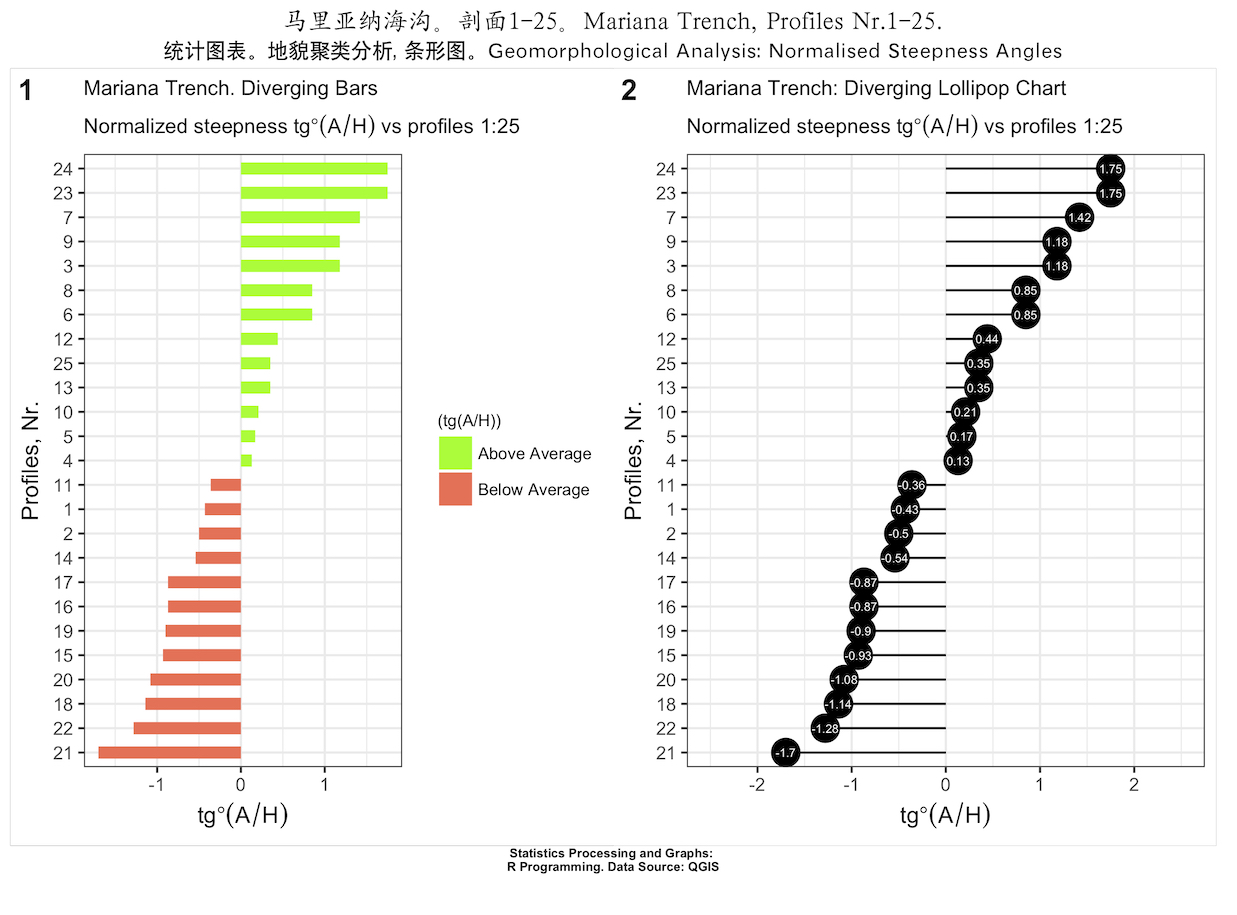
\includegraphics[width=8cm]{Fig-3-1.jpg}\caption{Visualization of the plot for normalized steepness: R.}
\end{figure}		
\end{frame}

\begin{frame}[fragile,shrink=10]\frametitle{R code to calculate normalized steepness by \{ggplot\} library: Parts 1 and 2}
\begin{lstlisting}[language=R]
# Part-1. Generate inicial data frame 
	# step-1. read in table
MorDF <- read.csv("Morphology.csv", header=TRUE, sep = ",")
head(MorDF)
summary(MorDF)
	# step-2. select two necessary columns from the initial table: numeric and symbol values. Generate from the them a new MDF data frame.
profile<- as.character(MorDF$profile)
tg_angle <- as.numeric(MorDF$tg_angle)
MDF<- data.frame(profile, tg_angle)
head(MDF)
# Part-2. change data frame MDF. 
	# step-3. Add new column for bathymetric profile names (here: by rows 1:25)
MDF$"profile name" <- rownames(MDF)  
	# step-4. re-calculate argumant values (by axis X) normalized by the difference between mean and standard deviation)
MDF$norm_tg_angle <- round((MDF$tg_angle - mean(MDF$tg_angle))/sd(MDF$tg_angle), 2)  # compute normalized tg_angle
	# step-5. distribute values of the normalized argument on "above" and "below" mean
MDF$angle_type <- ifelse(MDF$norm_tg_angle < 0, "below", "above")  # above / below avg flag	
	# step-6. sort dataframe
MDF <- MDF[order(MDF$norm_tg_angle), ]  # sort
	# step-7. values by Y axis (here: profile names) convert onto factor 
MDF$"profile name" <- factor(MDF$"profile name", levels = MDF$"profile name")  # convert to factor to retain sorted order in plot.
class(MDF$profile name) # check up class 
# [1] "factor" - should be
MDF # look up new data frame (5 columns vs initial 2 columns)
\end{lstlisting}
\end{frame}

\begin{frame}[fragile,shrink=15]\frametitle{R code to calculate normalized steepness by \{ggplot\} library: Part 3, steps 8 and 9.}
\begin{lstlisting}[language=R]
# Part-3. draw 2 plots by data frame MDF created in Part-2.
	# step-8. Diverging Barcharts 
Diverging_Bars<- ggplot(MDF, aes(x = MDF$"profile name", y = MDF$norm_tg_angle, label = MDF$norm_tg_angle)) + 
  geom_bar(stat='identity', aes(fill = MDF$angle_type), width=.5) +
  xlab("Profiles, Nr.") +
  ylab(expression(tg*degree*(A/H))) +
  scale_fill_manual(name="(tg(A/H))", 
        labels = c("Above Average", "Below Average"), 
        values = c("above"="lawngreen", "below"="coral1")) + 
  labs(title= "Mariana Trench. Diverging Bars",
  	subtitle=expression(paste("Normalized steepness ", tg*degree*(A/H), " vs profiles 1:25"))) + 
  coord_flip() +
  theme(plot.title = element_text(size = 10), 
    	legend.title = element_text(size=8), legend.text = element_text(colour="black", size = 8)) 
Diverging_Bars   
	# step-9. Plotting "Lollipop Chart"
Lollipop <- ggplot(MDF, aes(x = MDF$"profile name", y = MDF$norm_tg_angle, label = MDF$norm_tg_angle)) +    
	xlab("Profiles, Nr.") +
	ylab(expression(tg*degree*(A/H))) +
	geom_point(stat='identity', fill="black", size=6)  +   
	geom_segment(aes(y = 0, x = MDF$"profile name", yend = MDF$norm_tg_angle, xend = MDF$"profile name"), color = "black") +   
	geom_text(color="white", size=2) +   
	labs(title="Mariana Trench: Diverging Lollipop Chart",          
	subtitle=expression(paste("Normalized steepness ", tg*degree*(A/H), " vs profiles 1:25"))) +
	ylim(-2.5, 2.5) +   
coord_flip() +
    theme(plot.title = element_text(size = 10), legend.title = element_text(size=8), 
    		legend.text = element_text(colour="black", size = 8) ) 
Lollipop
\end{lstlisting}
\end{frame}

\begin{frame}[fragile]\frametitle{R code to calculate normalized steepness by \{ggplot\} library: Part 3, steps 10 and 11}
\begin{lstlisting}[language=R]
	# step-10. place both pots on one layout
figure <-plot_grid(Diverging_Bars, Lollipop, labels = c("1", "2"), ncol = 2, nrow = 1)
	# step-11. add common title, subtitle, subscript
LollipopBar <- figure +						
	labs(title="Mariana Trench, Profiles Nr.1-25.", 
	subtitle = "Geomorphological Analysis: Normalised Steepness Angles",
	caption = "Statistics Processing and Graphs: \nR Programming. Data Source: QGIS") +
	theme(plot.margin = margin(5, 10, 20, 5),
		plot.title = element_text(margin = margin(t = 0, r = 20, b = 5, l = 0), family = "Kai", face = "bold", size = 12), 
		plot.subtitle = element_text(margin = margin(t = 0, r = 20, b = 4, l = 0), family = "Hei", face = "bold", size = 10), 
		plot.caption = element_text(face = 2, size = 6), panel.background=ggplot2::element_rect(fill = "white"),
		legend.justification = "bottom", legend.position = "bottom",
		legend.box.just = "right", 
		legend.direction = "horizontal", 
		legend.box = "horizontal",
		legend.box.background = element_rect(colour = "honeydew4",size=0.2),
		legend.background = element_rect(fill = "white"),
		legend.key.width = unit(1,"cm"), 
		legend.key.height = unit(.5,"cm"),
		legend.spacing.x = unit(.2,"cm"), legend.spacing.y = unit(.1,"cm"),
		legend.text = element_text(colour="black", size=6, face=1),
		legend.title = element_text(colour="black", size=6, face=1) )
LollipopBar
\end{lstlisting}
\end{frame}

\begin{frame}\frametitle{Strip Plots by Tectonic Plates}
\begin{figure}[H]
	\centering
		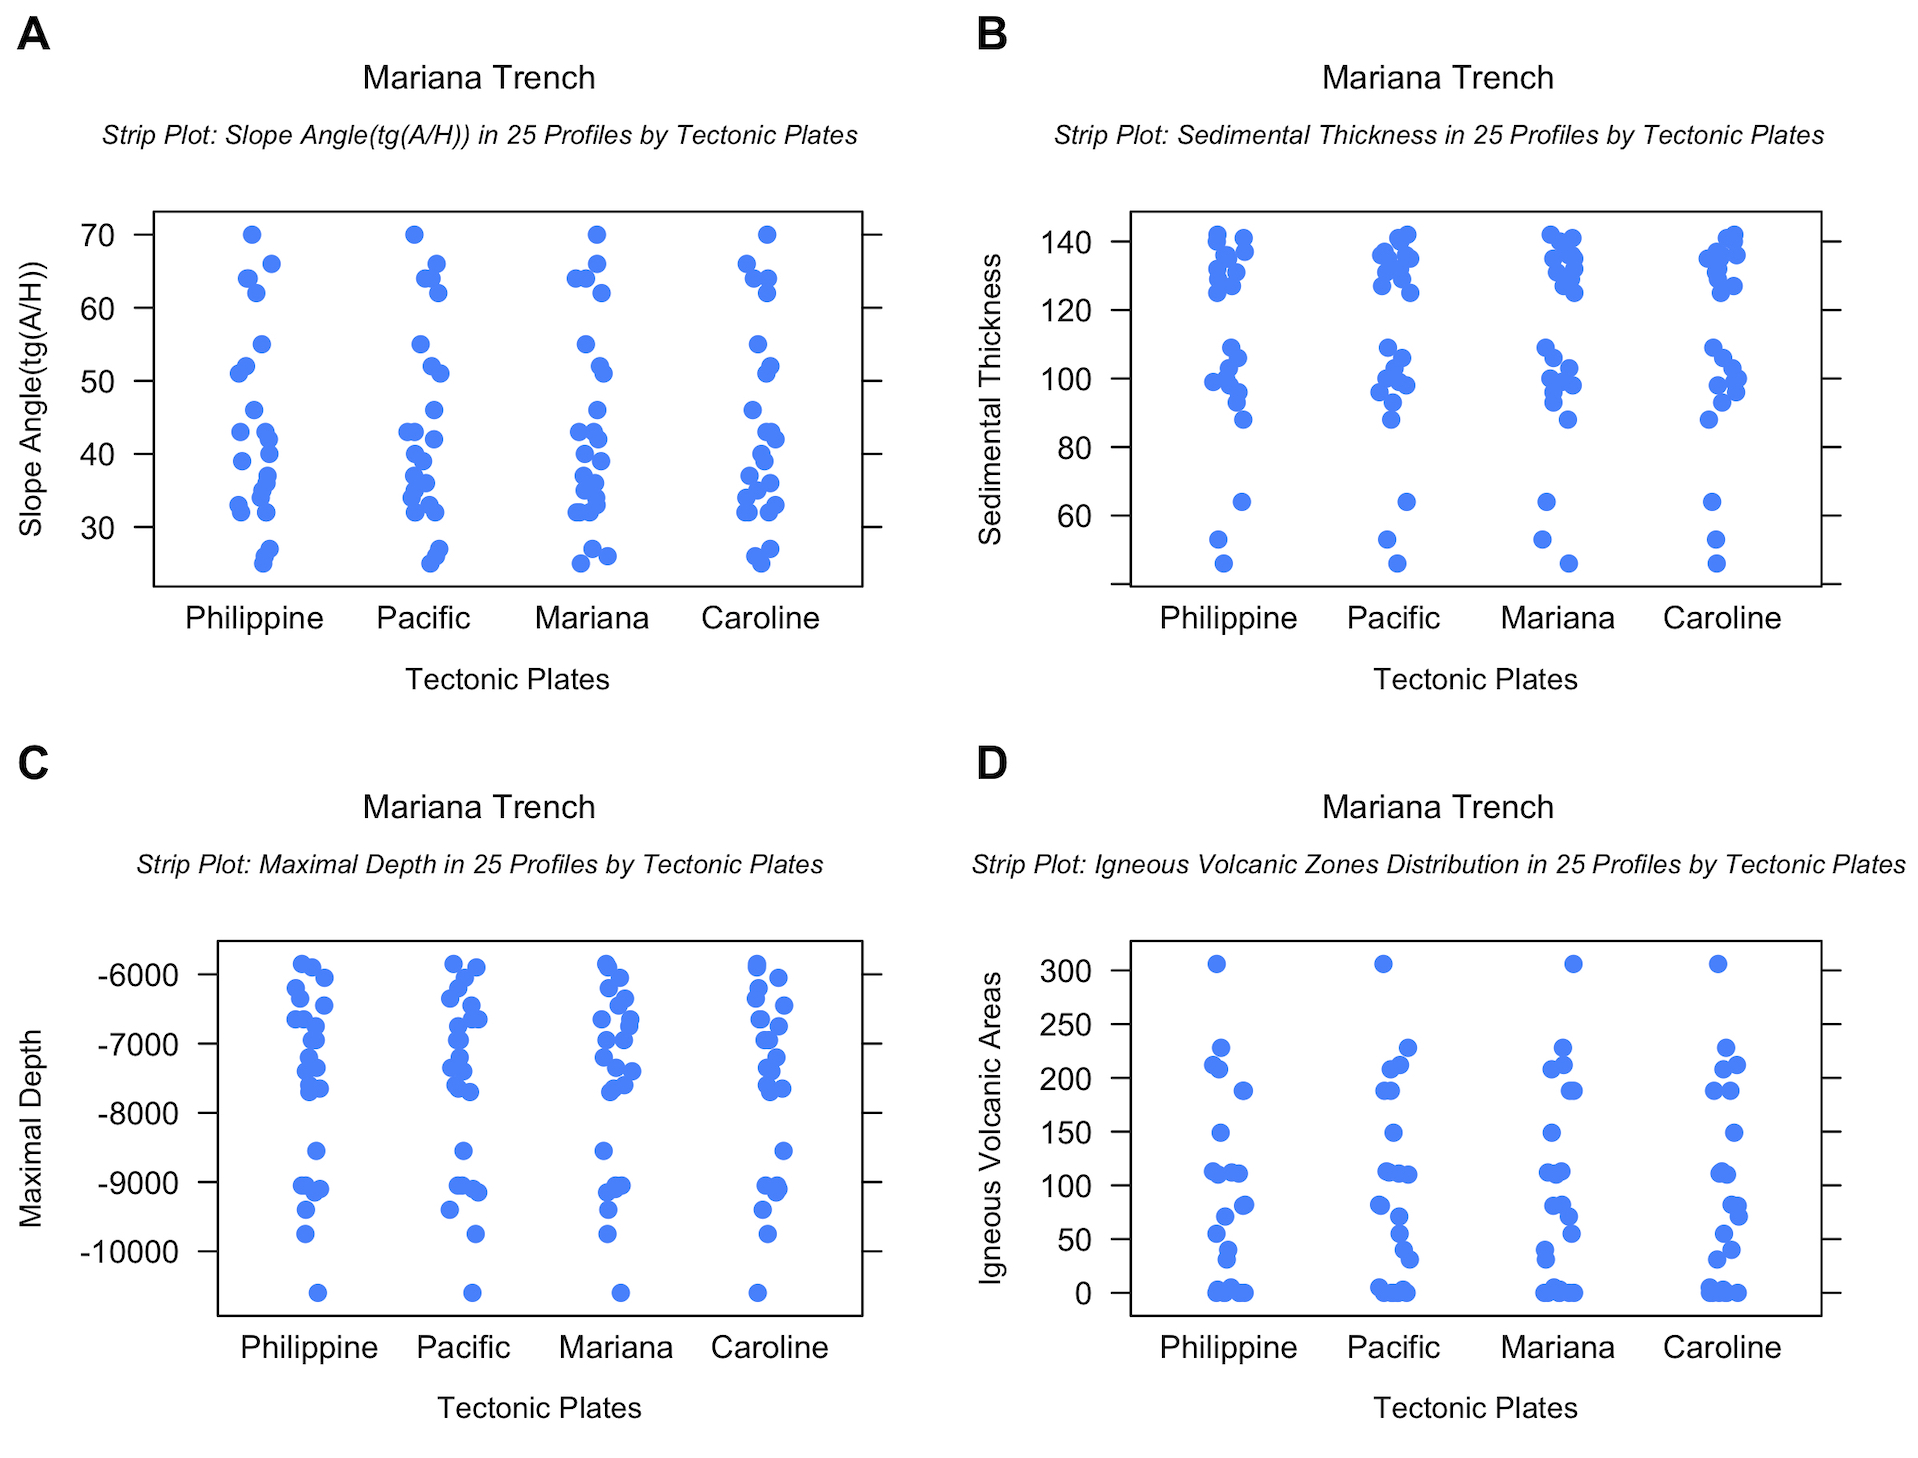
\includegraphics[width=8cm]{Fig-3-2.jpg}\caption{Combined plot for distribution of sediment thickness, geometric features (angle steepness and depth values) and volcanic areas}
\end{figure}		
\end{frame}

\begin{frame}[fragile,shrink=20]\frametitle{R code for multiple strip plots divided by groups\\ \{LatticeExtra\} library, Parts 1 and 2.}
\begin{lstlisting}[language=R]
# Multiple Strip plots  
# Part-1. prepare data frame
	# step-1. read in table with data. create initial data frame. clean up data frame from the NA values
MDepths <- read.csv("Morphology.csv", header=TRUE, sep = ",")
MDF <- na.omit(MDepths) 
row.has.na <- apply(MDF, 1, function(x){any(is.na(x))}) 
sum(row.has.na) 
head(MDF)
	# step-2. merge 4 columns with names of the plates into one named "tectonic plates" 
MDFt = melt(setDT(MDF), measure = patterns("^plate"), value.name = c("tectonic plates"))
head(MDFt)
	# step-3. indicate column with names of the tectonic plates as factor value (variable) 
MDFt$variable =as.factor(MDFt$variable)
levels(MDFt$variable)=c("Philippine" , "Pacific", "Mariana", "Caroline") # implicitly write the names of the 4 plates to be indicated on the X axis

# Part-2. generate well structured name (title + subtitle)
	# step-4. 
doubleTitle <- function(a,b) {     
	gTree(children=gList(         
		textGrob(a, gp=gpar(fontsize=10, fontface=1), y=0,              
			vp=viewport(layout.pos.row=1, layout.pos.col=1)),         
		textGrob(b, gp=gpar(fontsize=8, fontface=3), y=0,              
			vp=viewport(layout.pos.row=2, layout.pos.col=1))     
		), vp=viewport(layout=grid.layout(nrow=2, ncol=1)), cl="doubletitle") 
	}  
	heightDetails.doubletitle <- function(x, recording=T) {     
		Reduce(`+`, lapply(x$children, grid:::heightDetails.text)) * 2 
	}
\end{lstlisting}
\end{frame}

\begin{frame}[fragile,shrink=20]\frametitle{R code for multiple strip plots divided by groups\\ \{LatticeExtra\} library, Part 3.}
\begin{lstlisting}[language=R]
# Part-3. Strip plot (vertical distribution of the values by 4 categories))
	# step-5. strip plot 
	# step 5.1 angle of steepness:
s1<- stripplot(slope_angle ~ variable,  data = MDFt, jitter.data = TRUE, pch = 20,  palette="Set2",
	xlab = list(label="Tectonic Plates", cex= 0.60), 
	ylab = list(label="Slope Angle(tg(A/H))", cex= 0.60), 
	main=doubleTitle("Mariana Trench","Slope Angle(tg(A/H)) in 25 Profiles by Tectonic Plates"))
s1		
	# step 5.2  sediments:
s2<- stripplot(sedim_thick ~ variable,  data = MDFt, jitter.data = TRUE, pch = 20,  
	xlab = list(label="Tectonic Plates", cex= 0.60), 
	ylab = list(label="Sedimental Thickness", cex= 0.60), 
	main=doubleTitle("Mariana Trench","Sedimental Thickness in 25 Profiles by Tectonic Plates"))
s2	
	# step 5.3  minimal depths:
s3<- stripplot(Min ~ variable,  data = MDFt, jitter.data = TRUE, pch = 20,  
	xlab = list(label="Tectonic Plates", cex= 0.60), 
	ylab = list(label="Maximal Depth", cex= 0.60), 
	main=doubleTitle("Mariana Trench","Maximal Depth in 25 Profiles by Tectonic Plates"))
s3		
	# step 5.4 zones of the submarine volcanoes:
s4<- stripplot(igneous_volc ~ variable,  data = MDFt, jitter.data = TRUE, pch = 20,
	xlab = list(label="Tectonic Plates", cex=0.60), 
	ylab = list(label="Igneous Volcanic Areas", cex= 0.60),
	main=doubleTitle("Mariana Trench","Igneous Volcanic Zones Distribution in 25 Profiles by Tectonic Plates"))
s4
	# collect all strip plots on one layout:
g<- grid.arrange(s1, s2, s3, s4, ncol = 2, top = grid::textGrob(label = "Statistics: R Programming. Data Source: QGIS", x=0.1, hjust=0, gp=gpar(fontfamily="serif",fontsize=8, fontface="bold")))
l <- as_ggplot(g) + 
	draw_plot_label(label = c("A", "B", "C", "D"), size = 10, x = c(0, 0.5, 0, 0.5), y = c(1, 1, 0.5, 0.5))
\end{lstlisting}
\end{frame}

\begin{frame}\frametitle{Multiple scatter plot}
\begin{figure}[H]
	\centering
		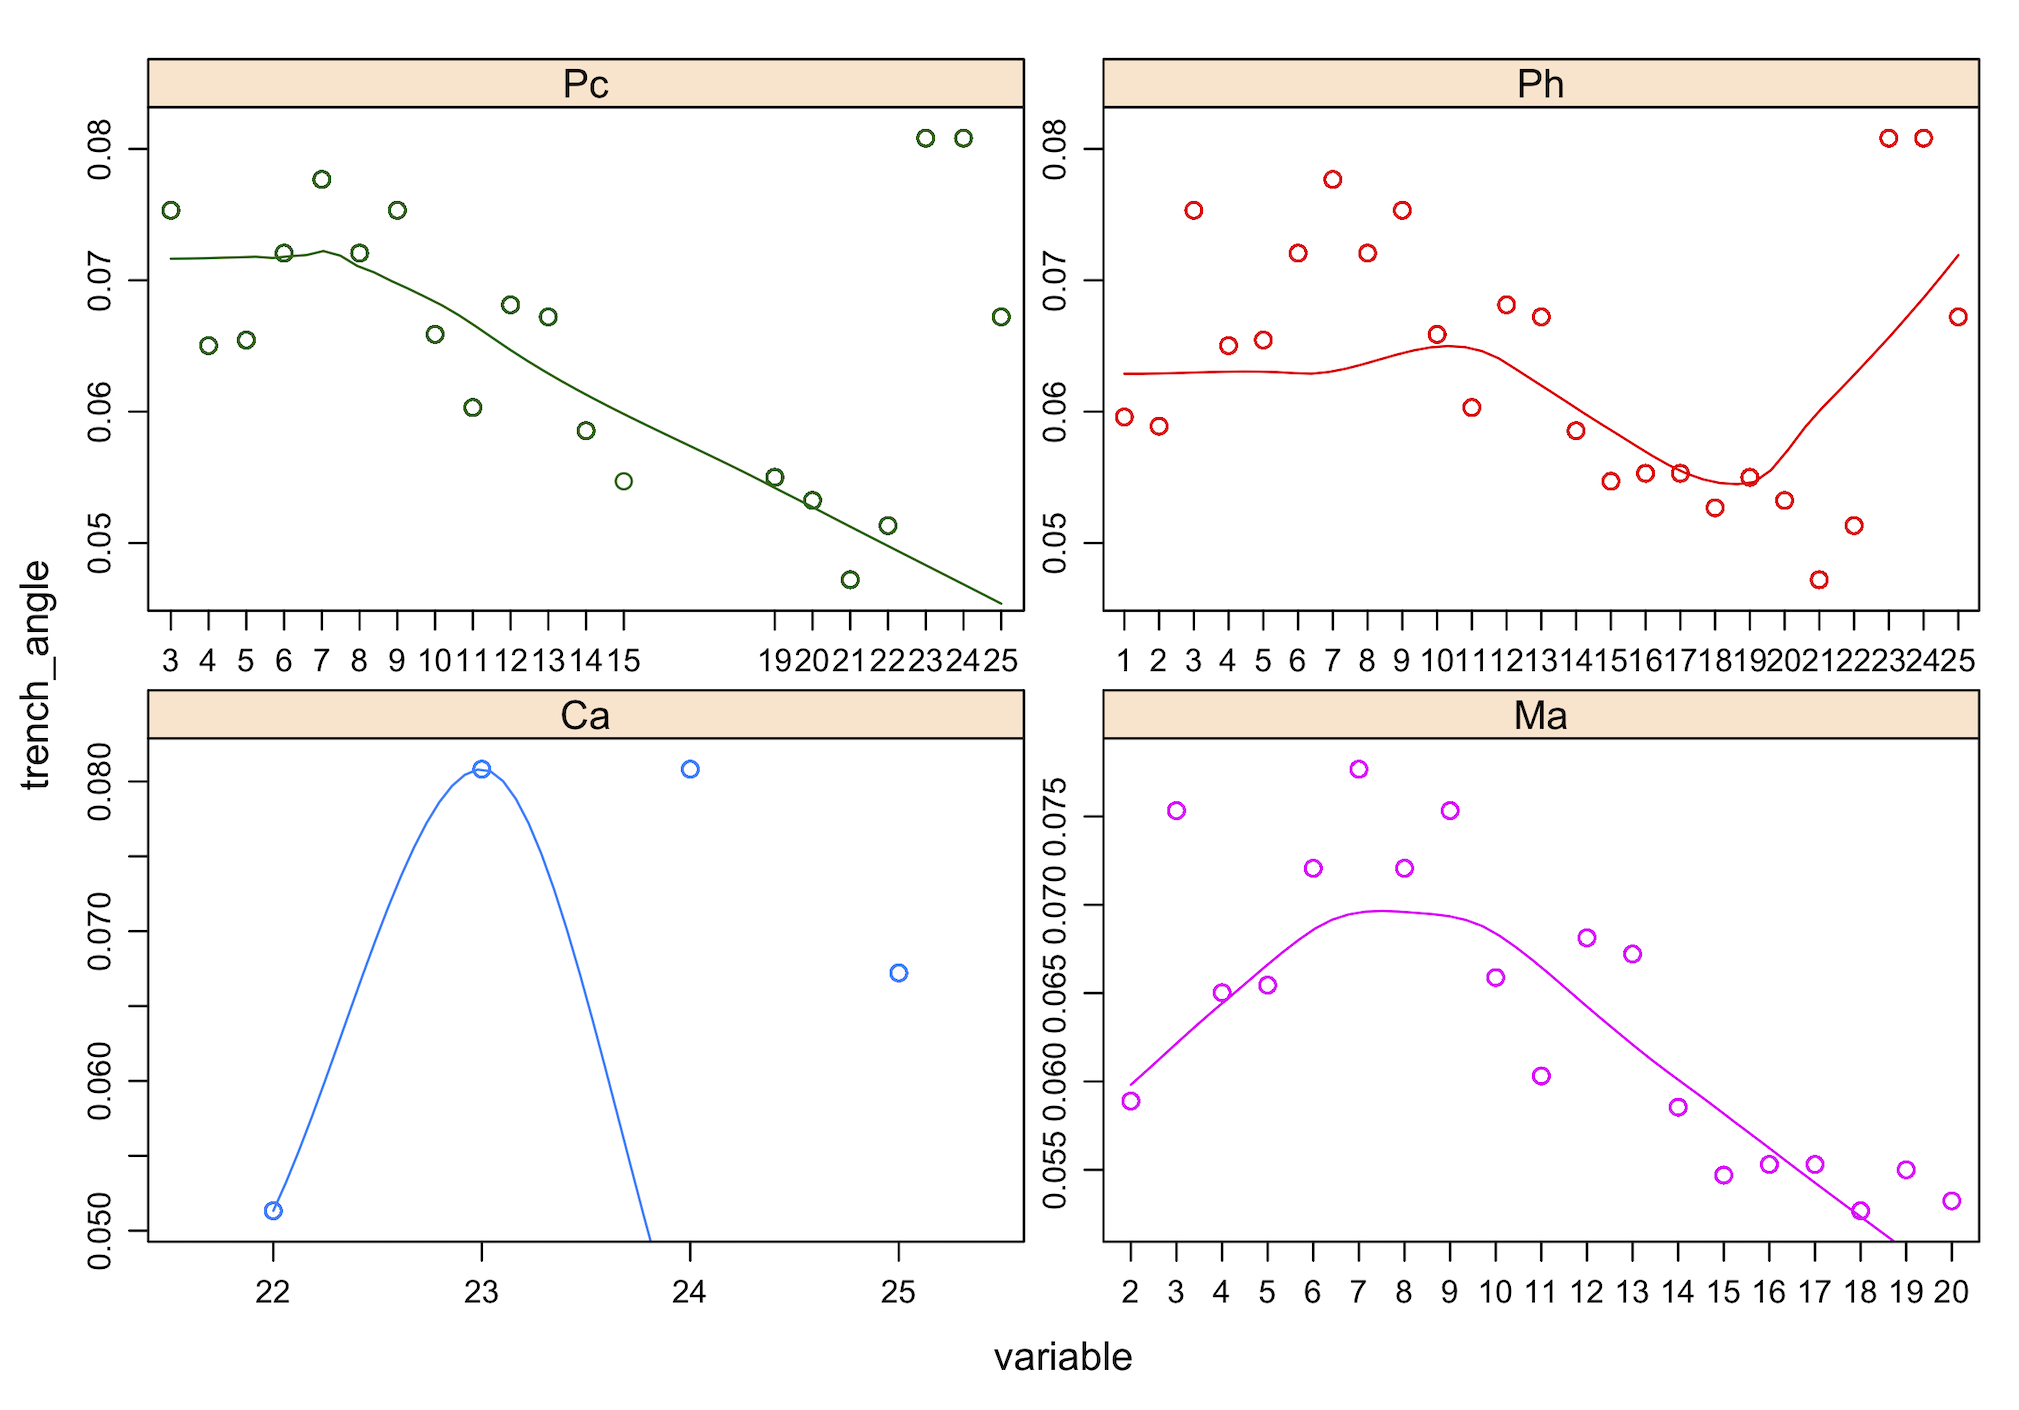
\includegraphics[width=9cm]{Fig-3-3.jpg}\caption{Multiple scatter plot: variation of the slope angle in the deepest point of 25 profiles by 4 tectonic plates, R.}
\end{figure}		
\end{frame}

\begin{frame}\frametitle{Multiple scatter plot}
\begin{figure}[H]
	\centering
		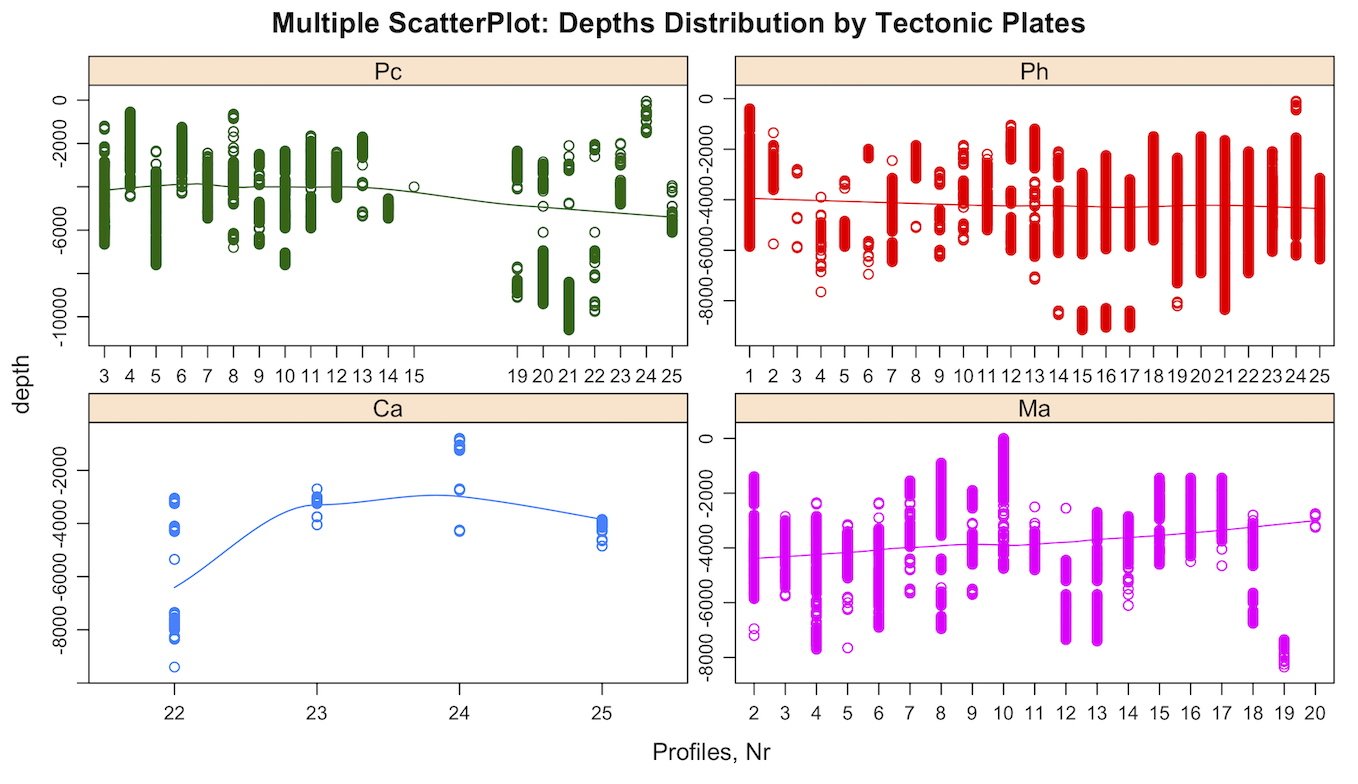
\includegraphics[width=10cm]{Fig-3-4.jpg}\caption{Multiple scatter plot: depth distribution in \\25 cross-section profiles by 4 tectonic plates, R.}
\end{figure}		
\end{frame}

\begin{frame}[fragile]\frametitle{R code for multiple panels by groups \\(tectonic plates, depths, slope angles)}
\begin{lstlisting}[language=R]
\subsection{R code for multiple panels by groups (tectonic plates, depths, slope angles)}\label{R:18}
Source data available on my \href{https://github.com/paulinelemenkova/R-17-Multiple-panels-by-groups}{GitHub}.
\begin{lstlisting}[language=R]
# Part-1. generate data frame. 
	# step-1.
MDepths <- read.csv("DepthTect.csv", header=TRUE, sep = ",")
MDFl <- na.omit(MDepths) 
row.has.na <- apply(MDFl, 1, function(x){any(is.na(x))}) # check up NA
sum(row.has.na) # sum up NA: [1] 0
head(MDFl) # look up clean data frame	
	# step-2. merge groups of categories by classes (here: tectonic plates, depths, slope angles)
DFDT = melt(setDT(MDFl), measure = patterns("^profile", "^tectonics", "^tg"), value.name = c("depth", "tectonics", "trench_angle"))
head(DFDT)
	# step-3. Multiple panels by groups: y ~ x | group generate multi-plot
p<- xyplot(depth ~ variable | tectonics, 
		group = tectonics, data = DFDT,
		type = c("p", "smooth"),
		scales = "free",
		main="Multiple ScatterPlot: Depths Distribution by Tectonic Plates",
		xlab="Profiles, Nr")
p
\end{lstlisting}
\end{frame}

\subsection{Correlation Analysis}

\begin{frame}\frametitle{Radar charts and Ternary diagrams}
\begin{figure}[H]
	\centering
		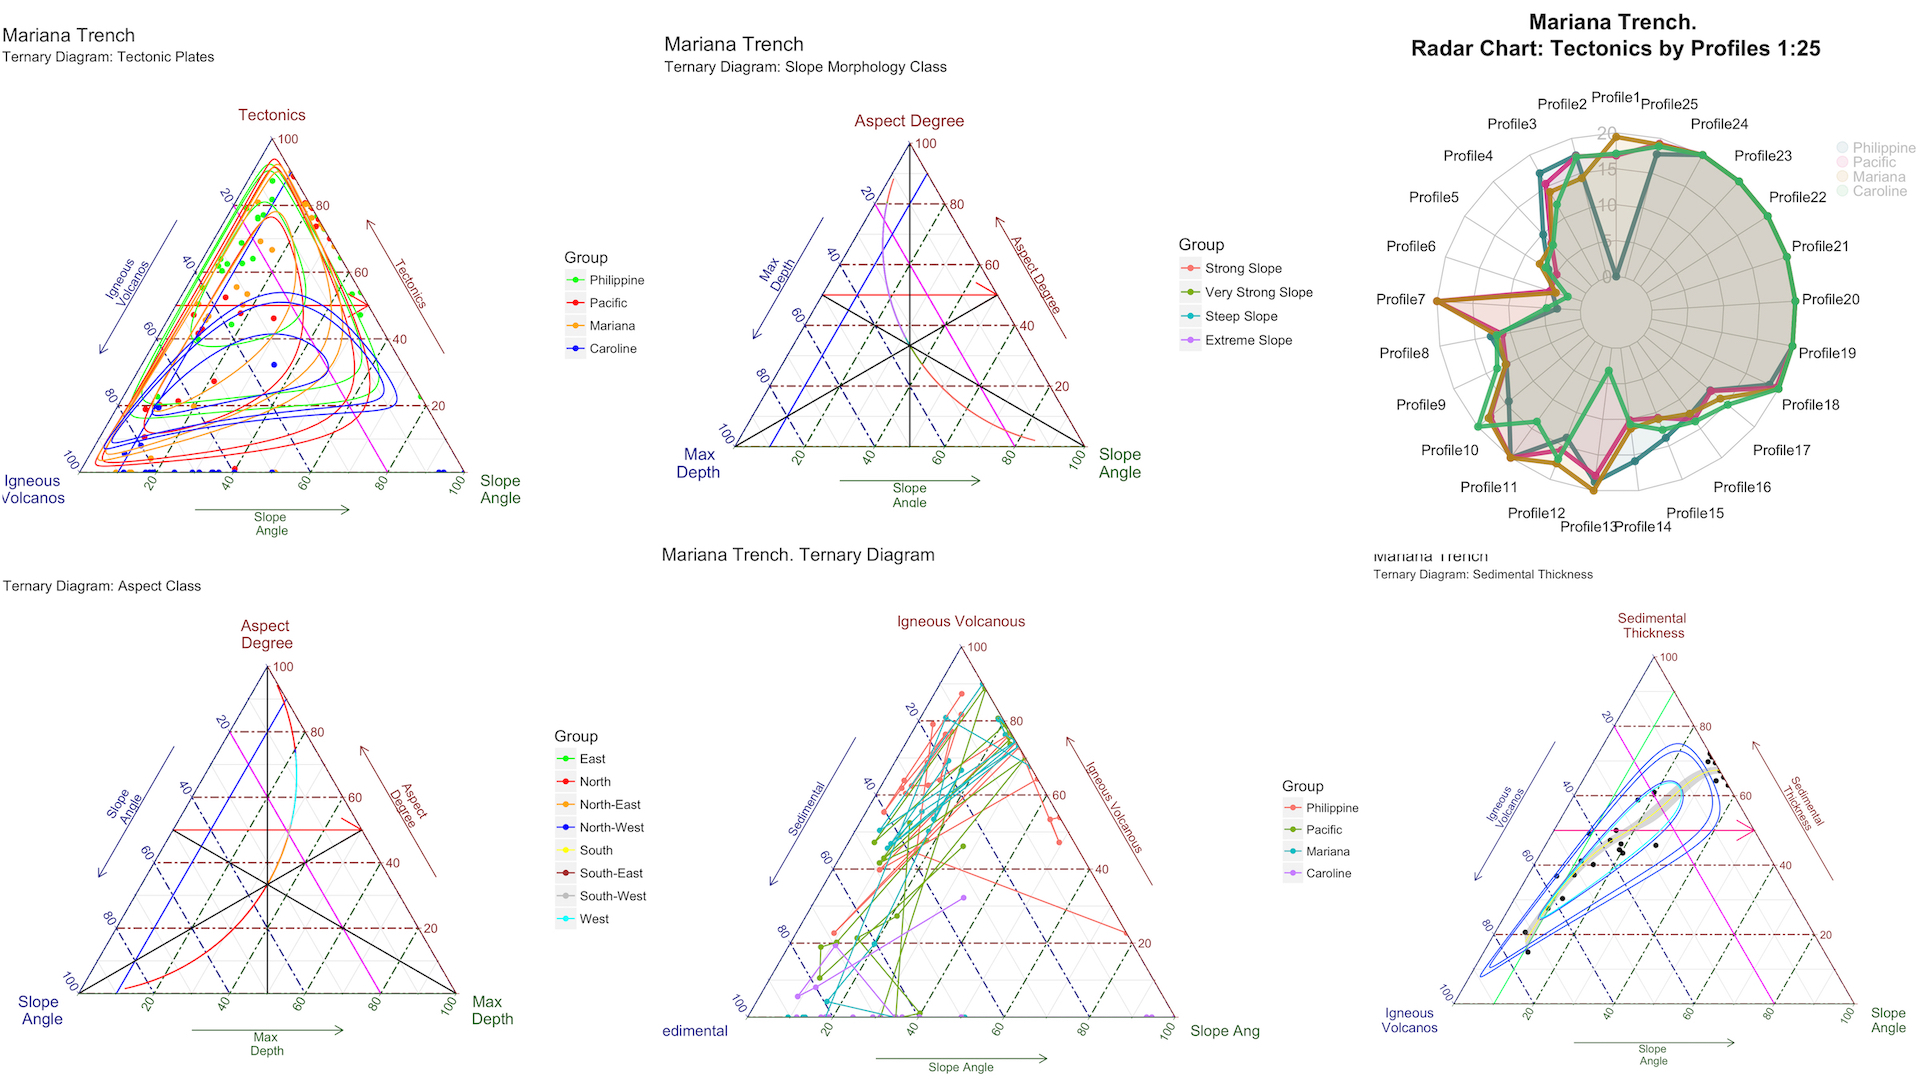
\includegraphics[width=10cm]{Fig-3-5.jpg}\caption{Radar charts and Ternary diagrams: \\correlations between environmental factors, R.}
\end{figure}		
\end{frame}

\begin{frame}[fragile,shrink=10]\frametitle{R code for ternary diagrams by \{ggtern\} library: \\Parts 1 and 2 (steps 1, 2, 3)}
Source data available on my \href{https://github.com/paulinelemenkova/29-R-Ternary}{GitHub}.
\begin{lstlisting}[language=R]
# Part 1: create data frame, delete NA values
	# step-1. read in table with data.
MDF <- read.csv("Morphology.csv", header=TRUE, sep = ",")
MDF <- na.omit(MDF) 
row.has.na <- apply(MDF, 1, function(x){any(is.na(x))})
sum(row.has.na) 
head(MDF) 
	# step-2. merge columns
MDTt = melt(setDT(MDF), measure = patterns("^plate"), value.name = c("tectonics"))
head(MDTt)
levels(MDTt$variable) = c("Philippine" , "Pacific", "Mariana", "Caroline")
Plates<- c("Philippine" , "Pacific", "Mariana", "Caroline")
# Part 2: draw ternary diagram for Mariana Trench
library(ggtern)  
 	# step-3. variant-1. 4 tectonic plates
MDTer <- data.frame( x = MDTt$igneous_volc, y = MDTt$tectonics, z = MDTt$slope_angle,
			Value = MDTt$slope_angle, Group = as.factor(MDTt$variable))
MT1<- ggtern(data= MDTer,aes(x,y,z,color = Group)) + 
	theme_rgbw() +
	geom_point() + 
	scale_color_manual(values = c("green" , "red", "orange", "blue")) + 
	labs(x="Igneous \nVolcanos", y="Tectonics", z="Slope \nAngle", title="Mariana Trench",
  		subtitle="Ternary Diagram: Tectonic Plates") +
  geom_Tline(Tintercept=.5,arrow=arrow(), colour='red') +
  geom_Lline(Lintercept=.2, colour='magenta') +
  geom_Rline(Rintercept=.1, colour='blue') +
  geom_confidence_tern() 
MT1
\end{lstlisting}
\end{frame}

\begin{frame}[fragile]\frametitle{R code for ternary diagrams by \{ggtern\} library: step 4}
\begin{lstlisting}[language=R]
	# step-4. variant-2. by morphology
levels(MDTt$morph_class) = c("Strong Slope", "Very Strong Slope", "Steep Slope", "Extreme Slope")
MDTM <- data.frame(
		x = MDTt$Min,
		y = MDTt$aspect_degree,
		z = MDTt$slope_angle,
		Value = MDTt$slope_angle,
		Group = as.factor(MDTt$morph_class))
MT2<- ggtern(data= MDTM,aes(x,y,z,color=Group), show.legend=TRUE) + 
	theme_rgbw() +
	geom_point() + 
	geom_path() + 
	labs(x="Max \nDepth",
		y="Aspect Degree",
		z="Slope\nAngle",
  		title="Mariana Trench",
  		subtitle="Ternary Diagram: Slope Morphology Class") +
  geom_Tline(Tintercept=.5,arrow=arrow(), colour='red') +
  geom_Lline(Lintercept=.2, colour='magenta') +
  geom_Rline(Rintercept=.1, colour='blue') +
  geom_confidence_tern() +
  geom_Tisoprop(value=0.5) +
  geom_Lisoprop(value=0.5) +
  geom_Risoprop(value=0.5)
MT2
\end{lstlisting}
\end{frame}

\begin{frame}[fragile]\frametitle{R code for ternary diagrams by \{ggtern\} library: step 5}
\begin{lstlisting}[language=R]
	# step-5. variant-3 by slope aspect
MDTAs <- data.frame(
			x = MDTt$slope_angle,
			y = MDTt$aspect_degree,
			z = MDTt$Min,
			Value = MDTt$aspect_degree,
			Group = as.factor(MDTt$aspect_class))
MT3<- ggtern(data = MDTAs,aes(x,y,z,color = Group)) + 
	theme_rgbw() +
	geom_point() + 
	scale_color_manual(values = c("green", "red", "orange", "blue", "yellow" , "brown", "grey", "cyan")) + 
	labs(x="Slope \nAngle", size = 1, 
		y="Aspect \nDegree", 
		z="Max \nDepth",
  		title="Mariana Trench",
  		subtitle="Ternary Diagram: Aspect Class") +
  geom_Tline(Tintercept=.5,arrow=arrow(), colour='red') +
  geom_Lline(Lintercept=.2, colour='magenta') +
  geom_Rline(Rintercept=.1, colour='blue') +
  geom_confidence_tern() +
  geom_Tisoprop(value=0.5) +
  geom_Lisoprop(value=0.5) +
  geom_Risoprop(value=0.5) 
MT3
\end{lstlisting}
\end{frame}

\begin{frame}[fragile]\frametitle{R code for ternary diagrams by \{ggtern\} library: \\steps 6 and 7}
\begin{lstlisting}[language=R]
	# step-6. plotting ternaries
plot<- grid.arrange(MT1, MT2, MT3, newpage = TRUE, nrow = 1, ncol = 3, top="Mariana Trench")
	# step-7. variant-4. by sediment thickness layer
MD4 <- data.frame(
			x = MDTt$igneous_volc,
			y = MDTt$sedim_thick,
			z = MDTt$slope_angle,
			Value = MDTt$slope_angle)
MT4<- ggtern(data = MD4,aes(x,y,z), show.legend=TRUE) + 
	theme_rgbw() +
	geom_point() + 
#	geom_path(alpha = .5, lwd = 0.2) + 
	labs(x="Igneous \nVolcanos", size = 0.5,y="Sediment \nThickness",z="Slope \nAngle",
  		title="Mariana Trench",
  		subtitle="Ternary Diagram: Sediment Thickness") +
  geom_Tline(Tintercept=.5,arrow=arrow(), colour='deeppink') +
  geom_Lline(Lintercept=.2, colour='magenta') +
  geom_Rline(Rintercept=.1, colour='springgreen') +
  geom_confidence_tern() + 
  geom_smooth_tern(method = 'loess', size = .4, color = "yellow1") +
  geom_mean_ellipse (size = .5, color = "cyan")
MT4
figure <-plot_grid(MT1, MT2, MT3, MT4, labels = c("1", "2", "3", "4"), ncol = 2, nrow = 2)
\end{lstlisting}
\end{frame}

\begin{frame}\frametitle{Categorywise Bar Chart}
\begin{figure}[H]
	\centering
		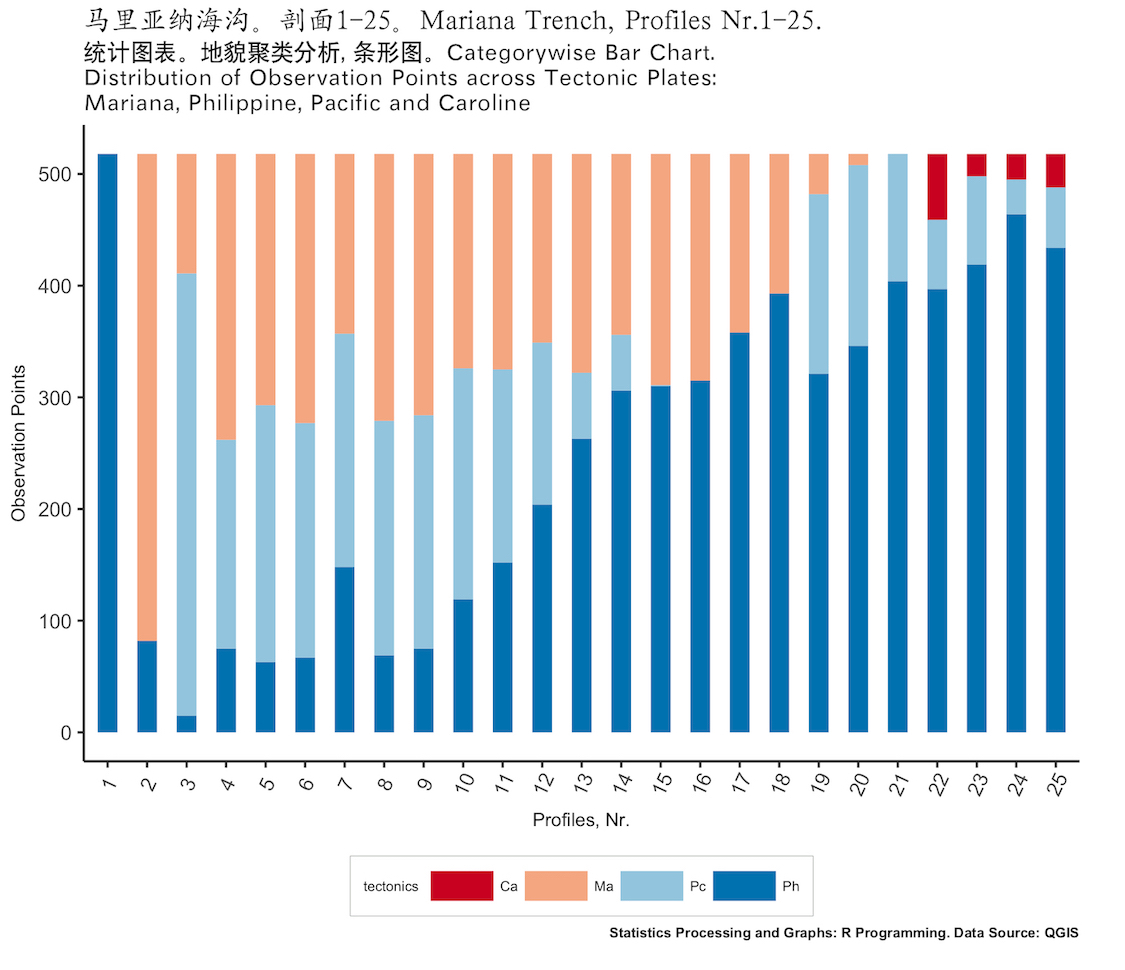
\includegraphics[width=7cm]{Fig-3-6.jpg}\caption{Categorywise bar chart to show quantitative data distribution across 4 tectonic plates, R.}
\end{figure}		
\end{frame}

\begin{frame}[fragile,shrink=20,]\frametitle{R code for categorywise bar charts}
\begin{lstlisting}[language=R]
# Part-1. Prepare data frame
	# step-1. read in table. create initial data frame
MDepths <- read.csv("DepthTect.csv", header=TRUE, sep = ",")
	# step-2. clean up data frame from NA values
MDF <- na.omit(MDepths) 
row.has.na <- apply(MDF, 1, function(x){any(is.na(x))}) # check up if there is any NA
sum(row.has.na) # sum up all NA, should be: [1] 0
head(MDF) # look up clean data frame 
	# step-3. merge table columns by 3 parameters, here: depths, tectonics, steepness angles. using melt от library(data.table)
DFDT = melt(setDT(MDF), measure = patterns("^profile", "^tectonics", "^tg"), value.name = c("depths", "tectonics", "angles"))
DFDT
# Part 2: draw categorywise bar chart, with colors by categories
	# step-4. draw diagram, add , добавляем legend, design
g <- ggplot(DFDT, aes(variable)) + 
	geom_bar(aes(fill = tectonics), width = 0.5, na.rm = TRUE) +    
	theme(axis.text.x = element_text(angle=65, vjust=0.6)) +  	   
	xlab("Profiles, Nr.") + ylab("Observation Points") + 
	labs(title="Mariana Trench, Profiles Nr.1-25.", 
	subtitle = "Categorywise Bar Chart. \nDistribution of Observation Points across Tectonic Plates: \nMariana, Philippine, Pacific and Caroline",
	caption = "Statistics Processing and Graphs: R Programming. Data Source: QGIS") +
	scale_fill_brewer(palette = "RdBu") +
	theme(
		plot.margin = margin(5, 10, 20, 5),
		plot.title = element_text(margin = margin(t = 0, r = 20, b = 5, l = 0), family = "Kai", face = "bold", size = 12), 
		plot.subtitle = element_text(margin = margin(t = 0, r = 20, b = 4, l = 0), family = "Hei", face = "bold", size = 10), 
		plot.caption = element_text(face = 2, size = 6), panel.background=ggplot2::element_rect(fill = "white"),
		axis.title.y = element_text(size = 8), axis.title.x = element_text(size = 8),
		legend.justification = "bottom", legend.position = "bottom",
		legend.box.just = "right",legend.direction = "horizontal",
		legend.box = "horizontal",legend.box.background = element_rect(colour = "honeydew4",size=0.2),
		legend.background = element_rect(fill = "white"),legend.key.width = unit(1,"cm"),
		legend.key.height = unit(.5,"cm"),legend.spacing.x = unit(.2,"cm"),
		legend.spacing.y = unit(.1,"cm"),legend.text = element_text(colour="black", size=6, face=1),
		legend.title = element_text(colour="black", size=6, face=1))
g
\end{lstlisting}
\end{frame}

\begin{frame}\frametitle{Circular plot: sediment thickness by 25 profiles, \\grouped by 4 tectonic plates (colored)}
\begin{figure}[H]
	\centering
		\subfloat {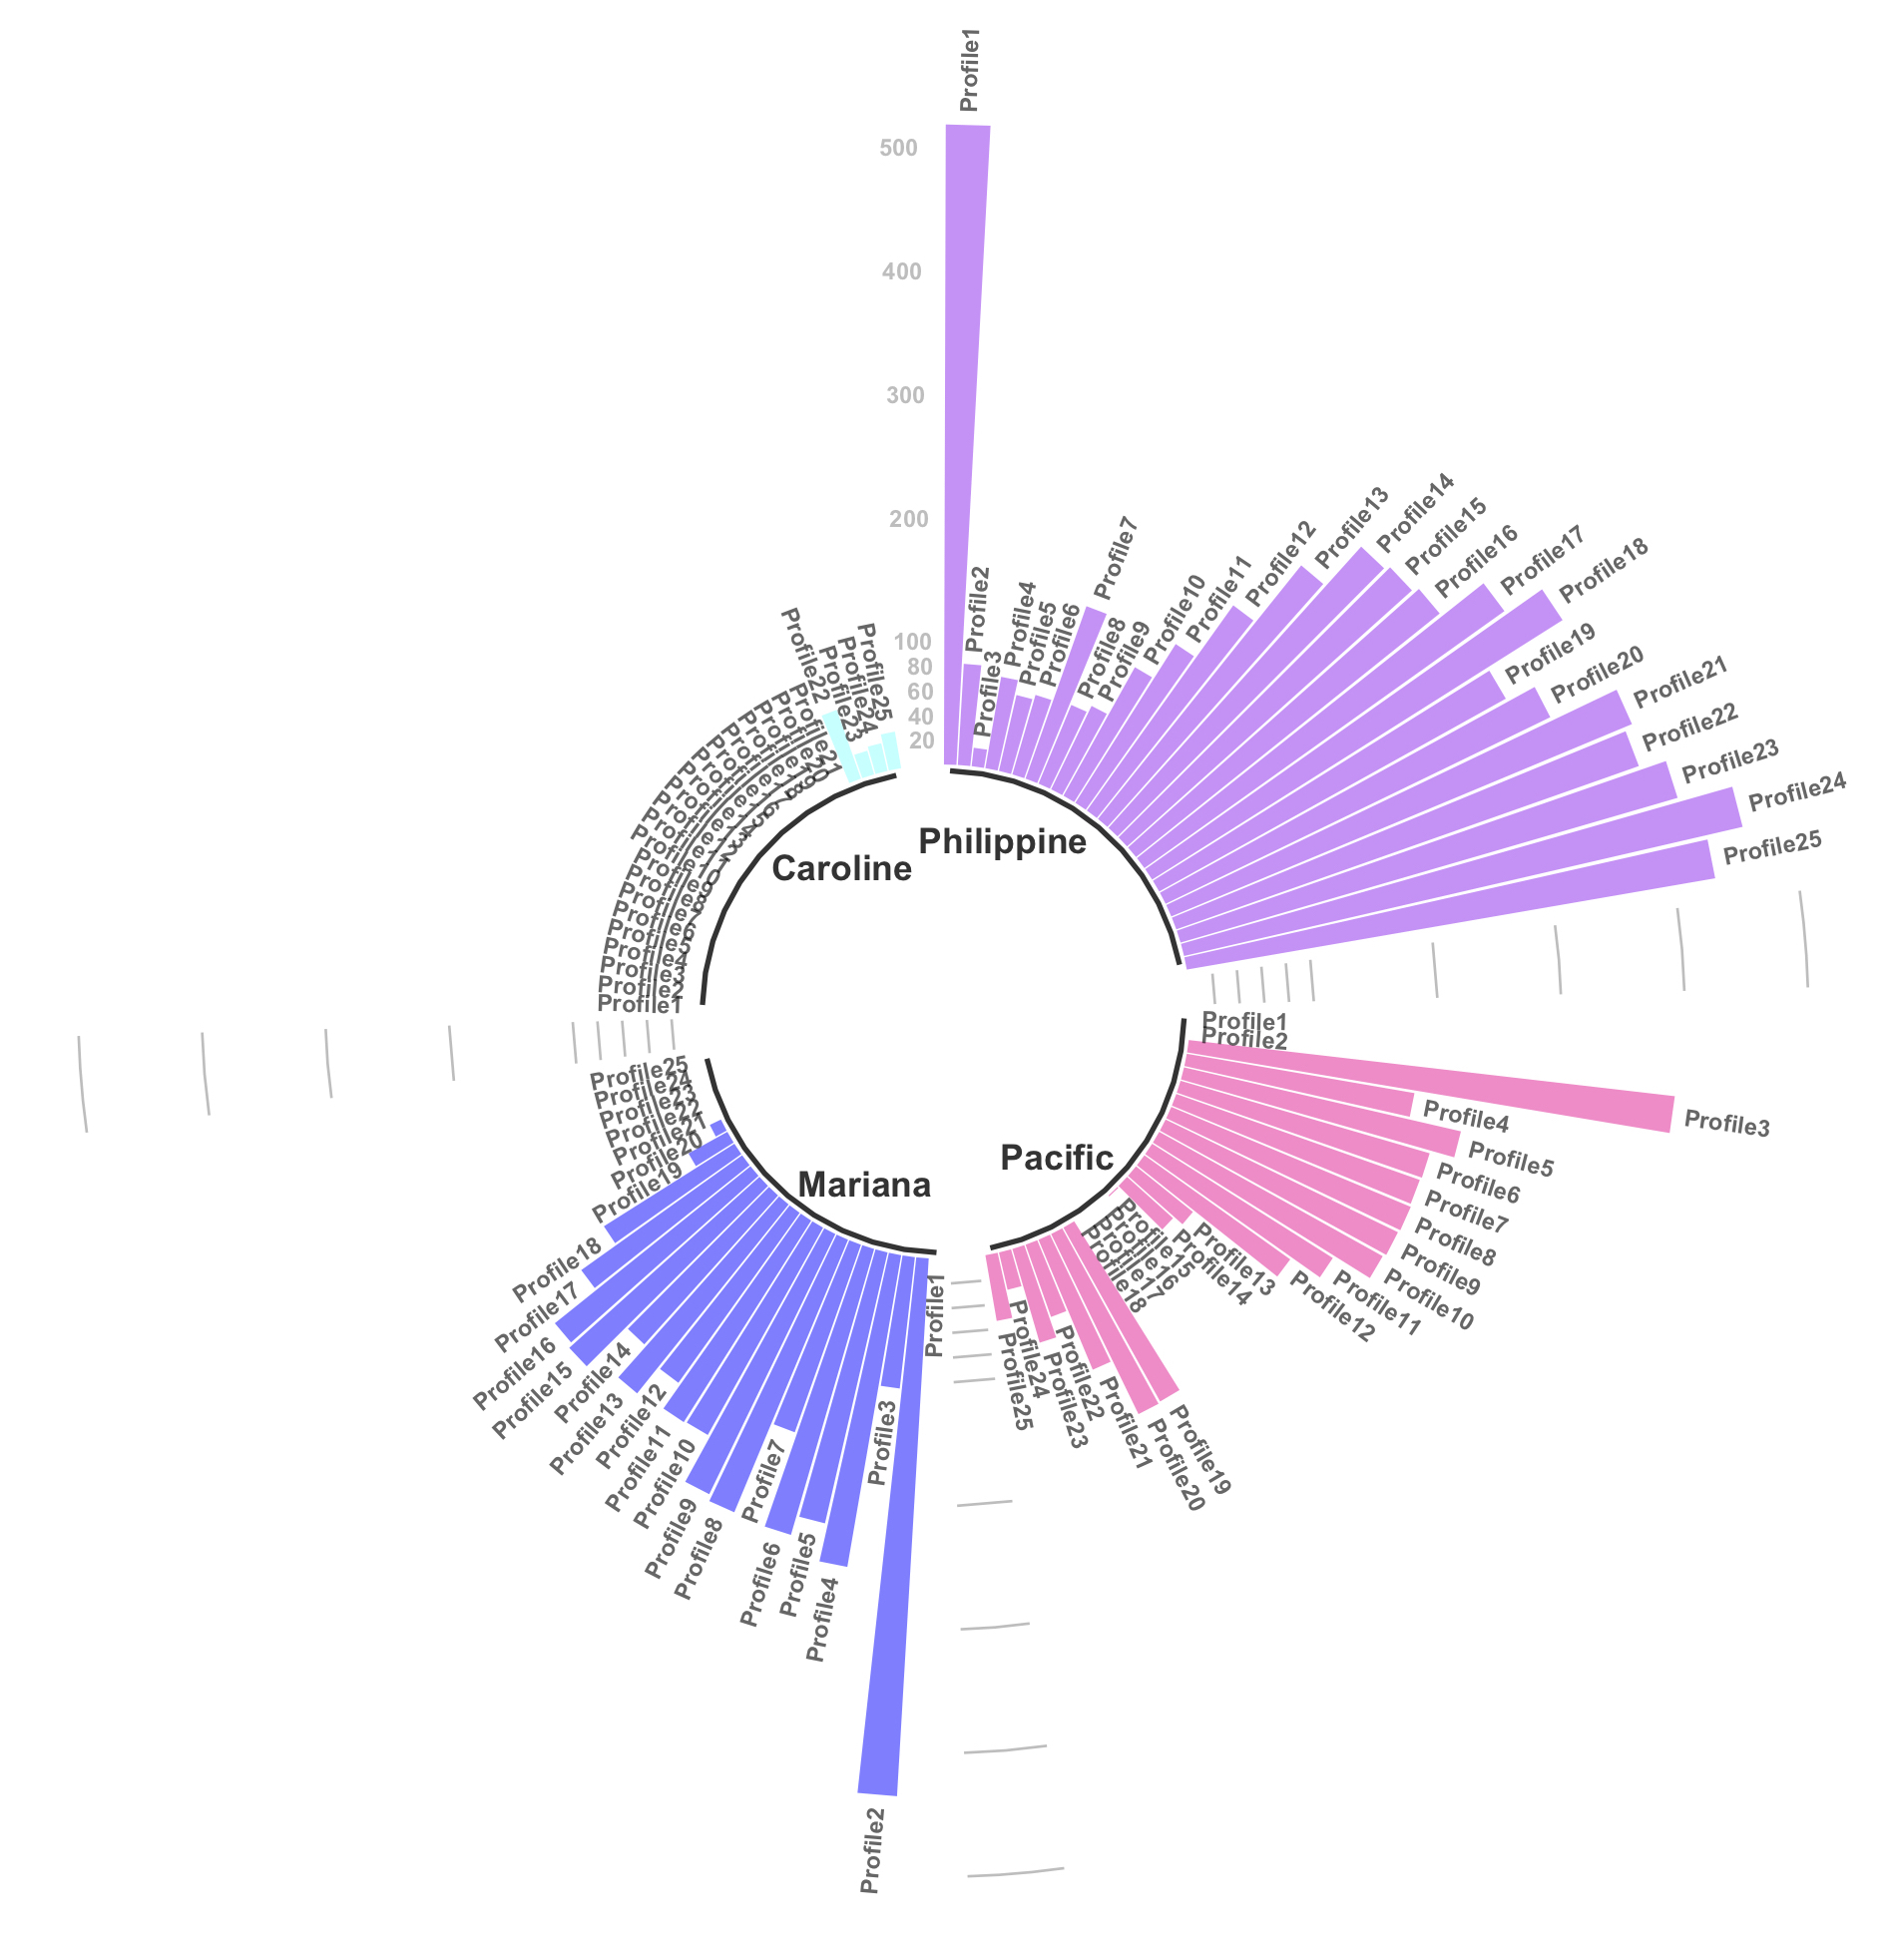
\includegraphics[width=5cm]{Fig-3-7b.jpg}}
			\hspace{5mm}
		\subfloat {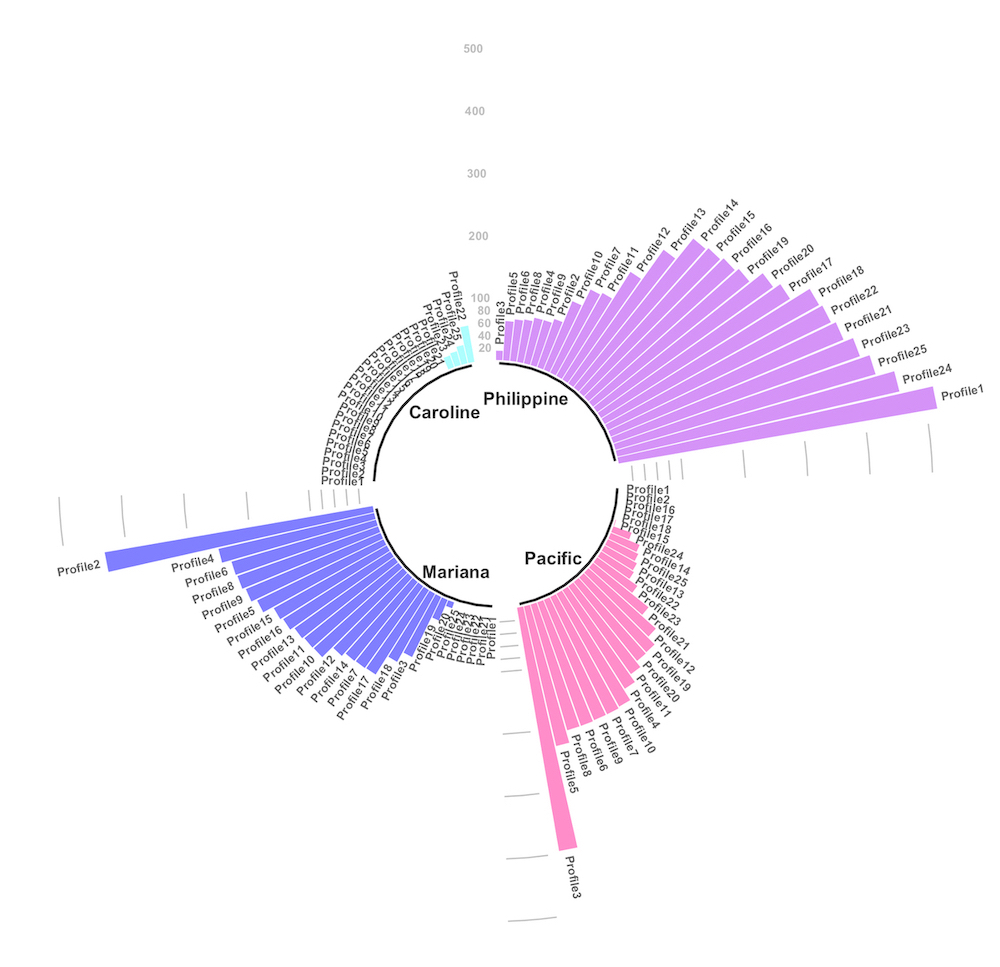
\includegraphics[width=5cm]{Fig-3-7c.jpg}}
		\caption{Circular plots to show . Left: unsorted, right: sorted, R.}
\end{figure}		
\end{frame}

\begin{frame}[fragile,shrink=10]\frametitle{R code for circular barplot by library \{tidyverse\} (1)}
\begin{lstlisting}[language=R]
# Part-1. Prepare data frame. 
	# step-1. read in table with data. create initial data frame. clean up from от NA
MDepths <- read.csv("Morphology.csv", header=TRUE, sep = ",")
MDF <- na.omit(MDepths) 
row.has.na <- apply(MDF, 1, function(x){any(is.na(x))}) 
sum(row.has.na) 
head(MDF)
	# step-2. merge categories by groups into classes (here: tectonics, depths, angles)
MDFt = melt(setDT(MDF), measure = patterns("^plate"), value.name = c("tectonics"))
head(MDFt)
	# step-3 create short data frame from 3 values (value - length of the 'flower' petal within the diagram)
data<- data.frame(
	id = MDFt$profile, # numbers as factor value, i.e. just as sequence 1:25
	individual = paste("Profile", seq(1,25), sep=""),
	group = MDFt$variable, # here: 4 tectonic plates
	value = MDFt$tectonics) # here: value of the sediment thickness layer (length of the petal of circle) 
levels(MDFt$variable) = c("Philippine" , "Pacific", "Mariana", "Caroline") # implicitly rename tectonic plates to be shown on the axis X
# Order data: 
data = data %>% arrange(group, value)
	# step-4 create empty column to add some space at the end of each group
empty_bar=3
to_add = data.frame( matrix(NA, empty_bar*nlevels(data$group), ncol(data)))
colnames(to_add) = colnames(data)
to_add$group=rep(levels(data$group), each=empty_bar)
data=rbind(data, to_add)
data=data %>% arrange(group)
data$id=seq(1, nrow(data))
\end{lstlisting}
\end{frame}

\begin{frame}[fragile]\frametitle{R code for circular barplot by library \{tidyverse\} (2)}
\begin{lstlisting}[language=R]
# Part-2. 
	# step-5 create tables for each petal getting the names from the data frame and the y position of each label
label_data = data 	
number_of_bar=nrow(label_data) # шаг-4 подсчитываем углы calculate the ANGLE of the labels 
angle = 90 - 360 * (label_data$id-0.5) /number_of_bar     # I substract 0.5 because the letter must have the angle of the center of the bars. Not extreme right(1) or extreme left (0)
label_data$hjust<-ifelse(angle < -90, 1, 0) # distribute labels on right and left 	
label_data$angle<-ifelse(angle < -90, angle+180, angle) # flip tables to make them readable 
# Part-3 Draw the circle 
	# step-6. prepare a data frame for the base lines
base_data=data %>% 
group_by(group) %>% 
summarize(start=min(id), end=max(id) - empty_bar) %>% 
rowwise() %>% 
mutate(title=mean(c(start, end)))
	# step-7. prepare a data frame for grid (scales)
grid_data = base_data
grid_data$end = grid_data$end[ c( nrow(grid_data), 1:nrow(grid_data)-1)] + 1
grid_data$start = grid_data$start - 1
grid_data=grid_data[-1,]	 
	# step-8. 
p <- ggplot(data, aes(x = as.factor(id), y = value, fill = group)) +
	geom_bar(aes(x = as.factor(id), y = value, fill = group), stat="identity", alpha=0.5) +	
#	scale_fill_distiller(palette = "Set1") +
  	scale_fill_manual(values = c("purple", "deeppink", "blue", "cyan")) +
\end{lstlisting}
\end{frame}

\begin{frame}[fragile,shrink=20]\frametitle{R code for circular barplot by library \{tidyverse\} (3)}
\begin{lstlisting}[language=R]
	# step-9. Add a val=100/75/50/25 lines to make sure barplots are over it.
	# here: draw come ticks of scale in the empty spaces between the petals from 25 to 100, further up to 500 by 100.
	geom_segment(data=grid_data, aes(x = end, y = 500, xend = start, yend = 500), colour = "grey", alpha=1, size=0.3 , inherit.aes = FALSE ) + 
	geom_segment(data=grid_data, aes(x = end, y = 400, xend = start, yend = 400), colour = "grey", alpha=1, size=0.3 , inherit.aes = FALSE ) +
	geom_segment(data=grid_data, aes(x = end, y = 300, xend = start, yend = 300), colour = "grey", alpha=1, size=0.3 , inherit.aes = FALSE ) +
	geom_segment(data=grid_data, aes(x = end, y = 200, xend = start, yend = 200), colour = "grey", alpha=1, size=0.3 , inherit.aes = FALSE ) +
	geom_segment(data=grid_data, aes(x = end, y = 100, xend = start, yend = 100), colour = "grey", alpha=1, size=0.3 , inherit.aes = FALSE ) +
	geom_segment(data=grid_data, aes(x = end, y = 80, xend = start, yend = 80), colour = "grey", alpha=1, size=0.3 , inherit.aes = FALSE ) +
	geom_segment(data=grid_data, aes(x = end, y = 60, xend = start, yend = 60), colour = "grey", alpha=1, size=0.3 , inherit.aes = FALSE ) +
	geom_segment(data=grid_data, aes(x = end, y = 40, xend = start, yend = 40), colour = "grey", alpha=1, size=0.3 , inherit.aes = FALSE ) +
	geom_segment(data=grid_data, aes(x = end, y = 20, xend = start, yend = 20), colour = "grey", alpha=1, size=0.3 , inherit.aes = FALSE ) +
	# step-10. add annotations of the scale ticks in one of the bars showing the value of each 100/75/50/25 lines
	annotate("text", x = rep(max(data$id),9), y = c(20, 40, 60, 80, 100, 200, 300, 400, 500), label = c("20", "40", "60", "80", "100", "200", "300", "400", "500") , color="grey", size = 2 , angle=0, fontface="bold", hjust=1) +	
	ylim(-200,550) + # ylim here 2 diameters of the circle - outer and inner
# here: ylim = 550, because all values of the tectonics do not overstep 550 (i.e. outer circle) 
# value -50 - diamcircleeter of the inner circle.
	#theme_minimal() +  
theme(
	legend.position = "none",
	axis.text = element_blank(),
	axis.title = element_blank(),
	plot.title = element_text(margin = margin(t = 0, r = 0, b = 0, l = 0), size = 10, face = "bold"),
	plot.margin = unit(rep(-1,4), "cm")) +
	coord_polar() + 
	geom_text(data = label_data, aes(x = id, y = value+10, label = individual, hjust=hjust), color="black", fontface="bold",alpha=0.6, size=2.0, angle= label_data$angle, inherit.aes = FALSE ) +
# Add base line information
	geom_segment(data = base_data, aes(x = start, y = -5, xend = end, yend = -5), colour = "black", alpha=0.8, size=0.6 , inherit.aes = FALSE )  +
	geom_text(data = base_data, aes(x = title, y = -18, label = group), hjust=c(1,1,0,0), colour = "black", alpha=0.8, size=3, fontface="bold", inherit.aes = FALSE)
p
\end{lstlisting}
\end{frame}

\begin{frame}\frametitle{Pairwise double-Y-axis}
\begin{figure}[H]
	\centering
		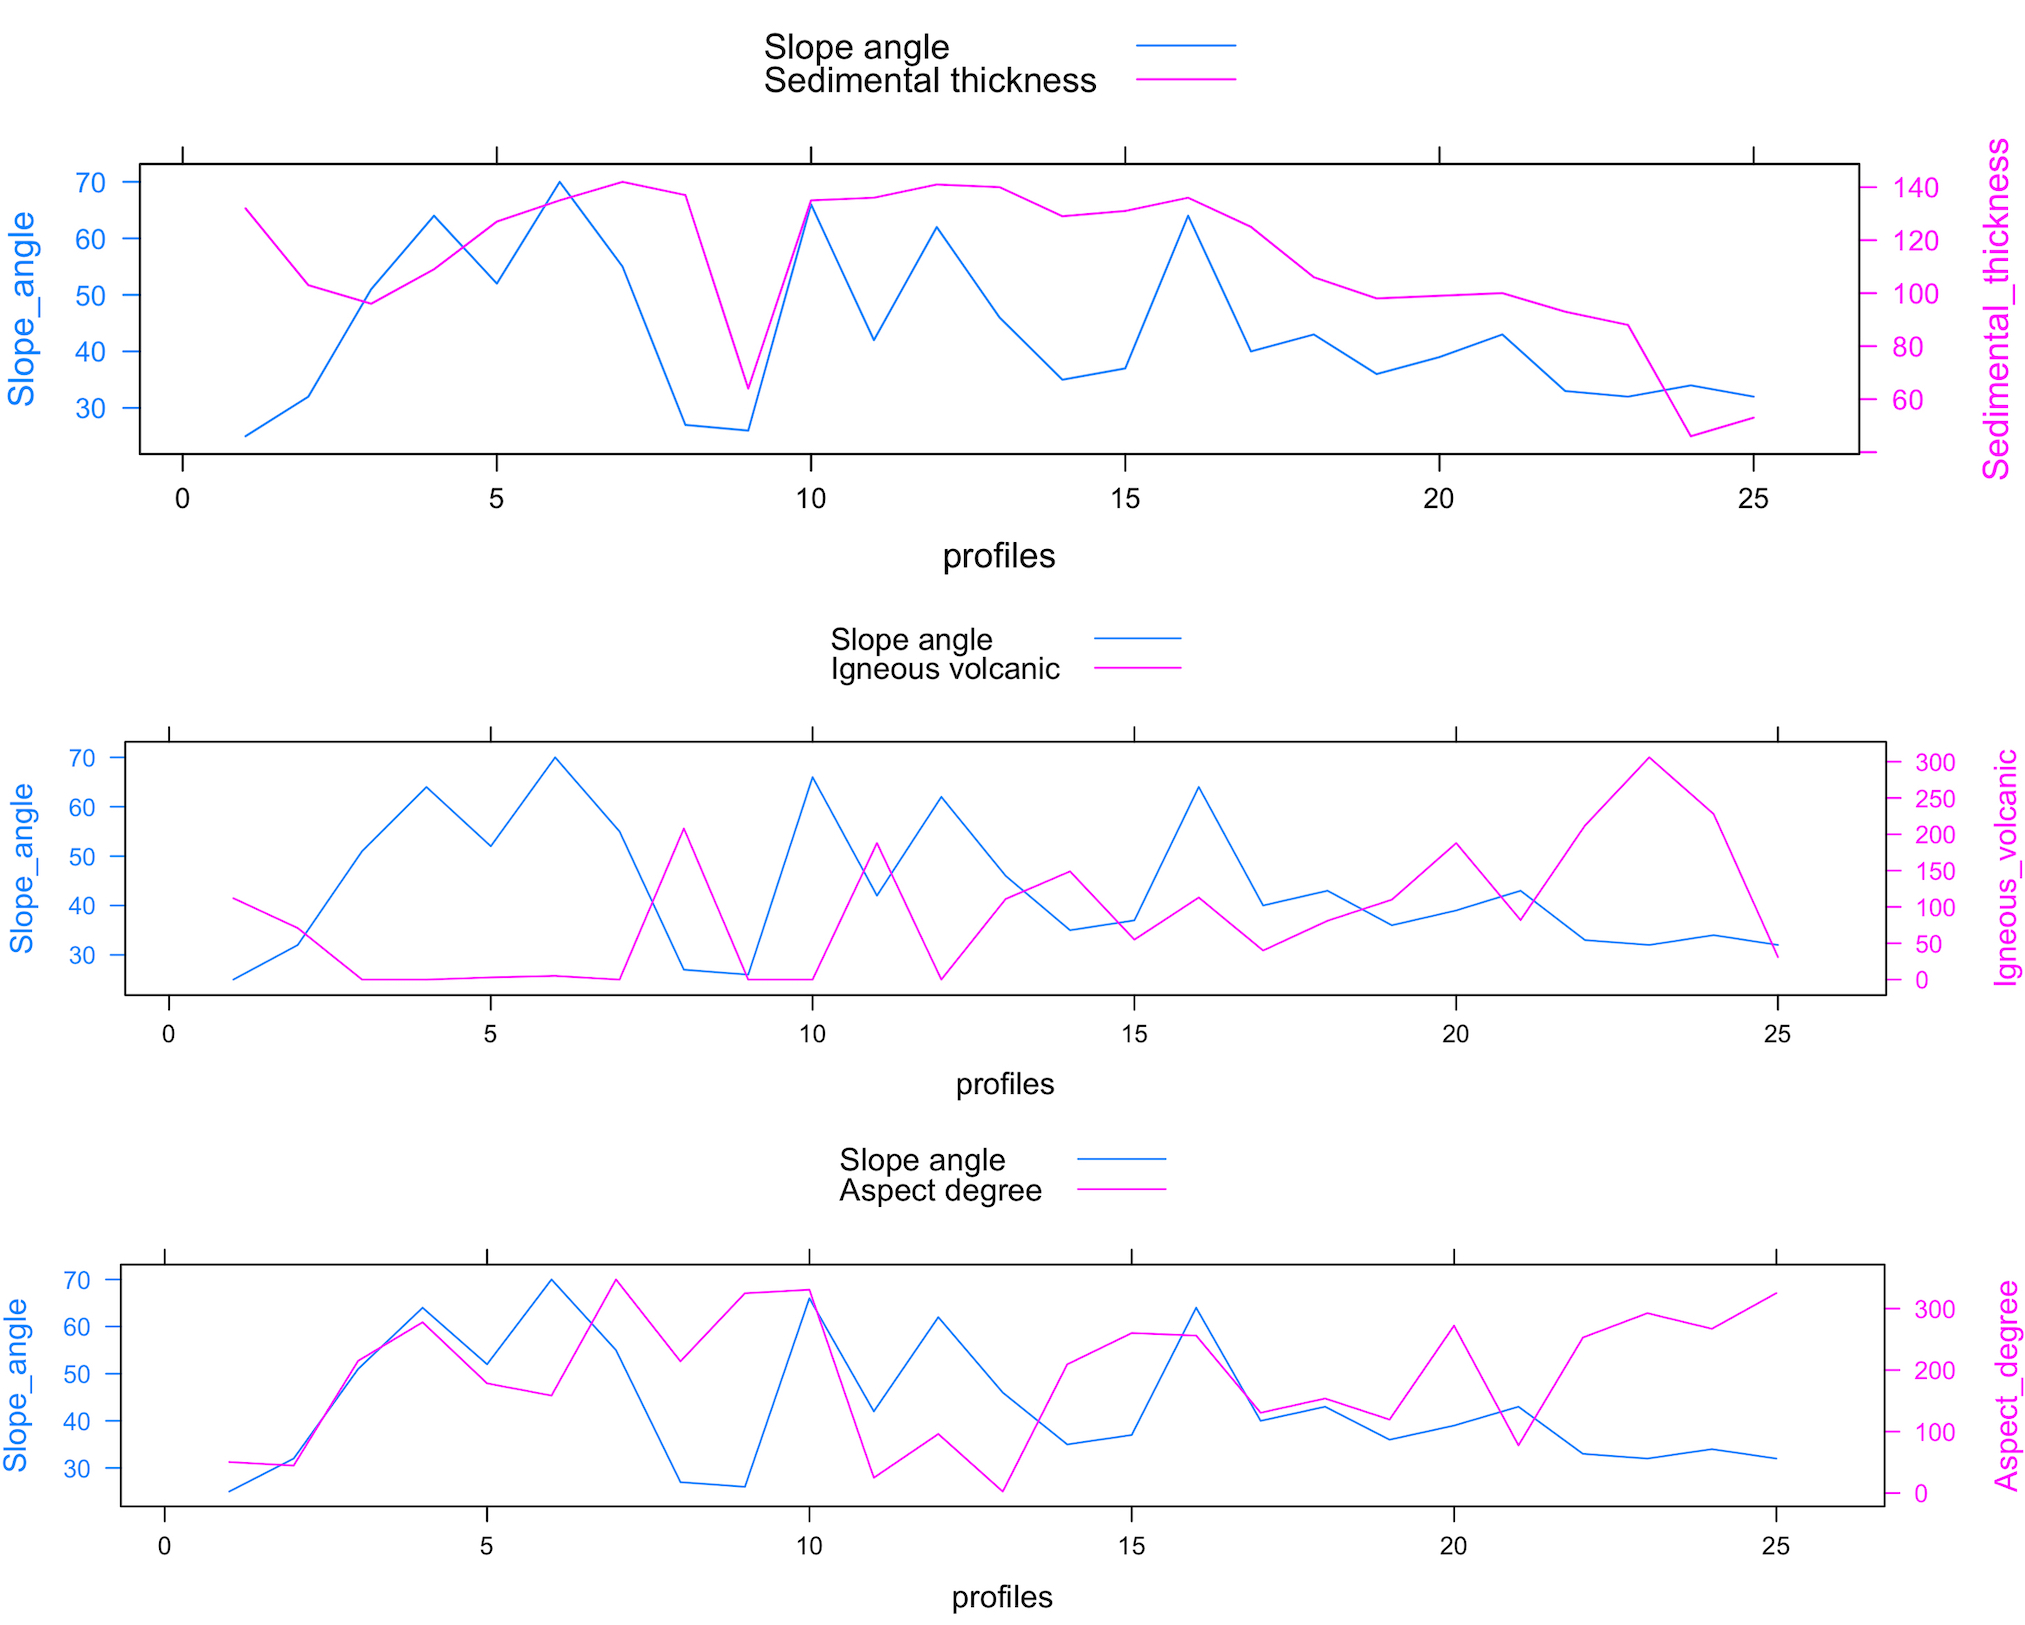
\includegraphics[width=7cm]{Fig-3-8a.jpg}
	\caption{Pairwise double-Y-axis}
\end{figure}		
\end{frame}

\begin{frame}[fragile]\frametitle{R code for double-Y axis by \{LatticeExtra\} library\\ Parts 1 and 2a}
\begin{lstlisting}[language=R]
	# Part-1. prepare data frame. 
	# step-1. read in table with data on geomorphology. Generate initial data frame
MDepths <- read.csv("Morphology.csv", header=TRUE, sep = ",")
	# step-2. clean up data frame from NA values
MDF <- na.omit(MDepths) 
row.has.na <- apply(MDF, 1, function(x){any(is.na(x))}) # check up if any NA area available
sum(row.has.na) # sum up all NA, should be: [1] 0
head(MDF) 
	# Part-2а. Draw 2 plots Y on one axis X "Slope angle", "Sediment thickness"
library(latticeExtra) 
	# step-3. generate selection of data for new data frame (only 3 useful values)
set.seed(1)
profiles = MDF$profile
Slope_angle = MDF$slope_angle
Sediment_thickness =  MDF$sedim_thick
data=data.frame(profiles, Slope_angle, Sediment_thickness)
	# step-4 two plots in one :
p<- xyplot(Slope_angle + Sediment_thickness ~ profiles, data, type = "l")
p		
	# step-5. plots 1 and 2 read into objects
obj1 <- xyplot(Slope_angle ~ profiles, data, type = "l" , lwd=1)
obj2 <- xyplot(Sediment_thickness ~ profiles, data, type = "l", lwd=1)
	# step-6. add 2nd axis Y:
doubleYScale(obj1, obj2, add.ylab2 = TRUE)
	# step-7. add legend:
p<- doubleYScale(obj1, obj2, text = c("Slope angle", "Sediment thickness"), add.ylab2 = TRUE) 
\end{lstlisting}
\end{frame}

\begin{frame}[fragile,shrink=20]\frametitle{R code for double-Y axis using  \{LatticeExtra\} library:\\ comparative analysis of variables. Part-2b}
\begin{lstlisting}[language=R]
	# Part-2b. Categories: "Slope angle", "Aspect degree" by bathymetric profiles
	# step-8. generate selection of data for new data frame (only 3 useful values)
set.seed(1)
profiles = MDF$profile
Slope_angle = MDF$slope_angle
Aspect_degree =  MDF$aspect_degree
data=data.frame(profiles, Slope_angle, Aspect_degree)
p<- xyplot(Slope_angle + Aspect_degree ~ profiles, data, type = "l")
p		
	# step-9. plots 1 and 2 read into objects
obj1 <- xyplot(Slope_angle ~ profiles, data, type = "l" , lwd=1)
obj2 <- xyplot(Aspect_degree ~ profiles, data, type = "l", lwd=1)
doubleYScale(obj1, obj2, add.ylab2 = TRUE)
	# step-10. add legend:
p1 <- doubleYScale(obj1, obj2, text = c("Slope angle", "Aspect degree") , add.ylab2 = TRUE)
	# Part-2c. Categories: "Slope angle", "igneous volcanic areas" by bathymetric profiles
	# step-10. generate selection of data for new data frame (only 3 useful values)
set.seed(1)
profiles = MDF$profile
Slope_angle = MDF$slope_angle
Igneous_volcanic =  MDF$igneous_volc
data=data.frame(profiles, Slope_angle, Igneous_volcanic)
	# step-11 plots together:
p<- xyplot(Slope_angle + Igneous_volcanic ~ profiles, data, type = "l")
p		
	# step-12. plots 1 and 2 read into objects, add 2nd axis Y:
obj1 <- xyplot(Slope_angle ~ profiles, data, type = "l" , lwd=1)
obj2 <- xyplot(Igneous_volcanic ~ profiles, data, type = "l", lwd=1) 
doubleYScale(obj1, obj2, add.ylab2 = TRUE)
	# step-13. add legend:
p2 <- doubleYScale(obj1, obj2, text = c("Slope angle", "Igneous volcanic") , add.ylab2 = TRUE)
p2
\end{lstlisting}
\end{frame}

\begin{frame}\frametitle{Ranking dot plots by data grouping}
\begin{figure}[H]
	\centering
		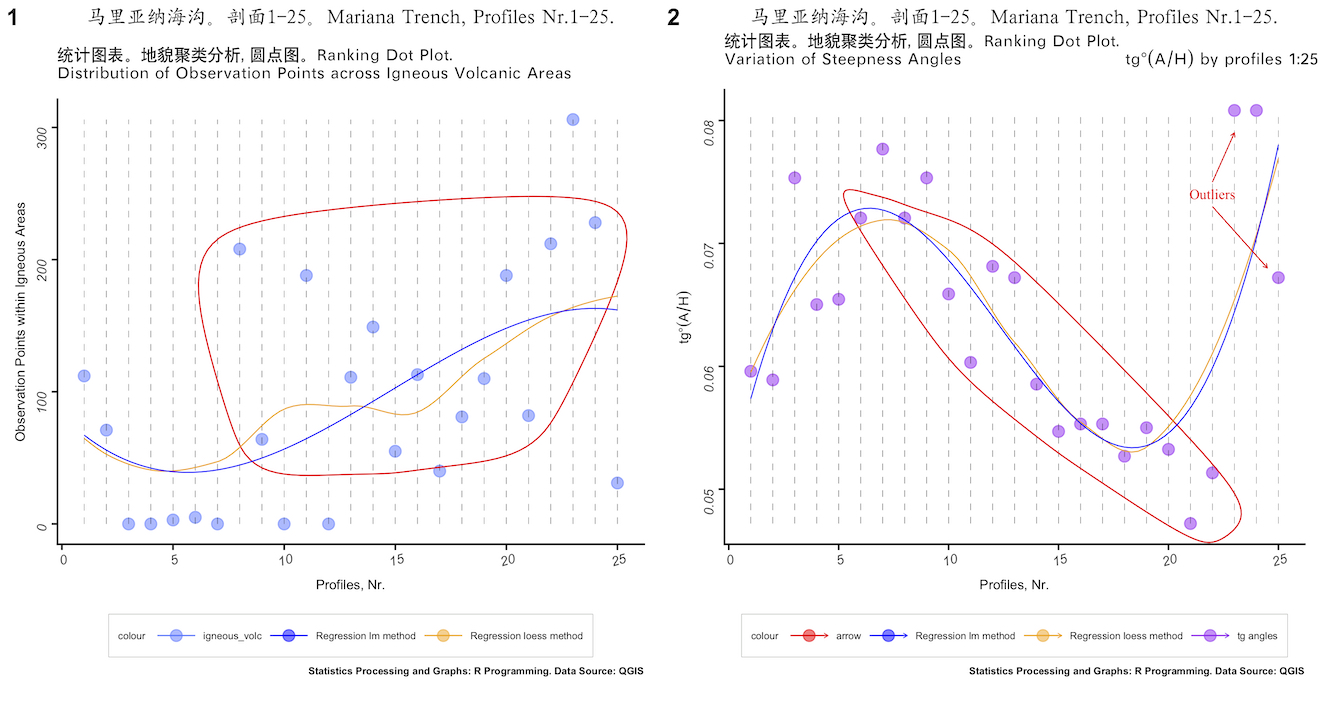
\includegraphics[width=11cm]{Fig-3-8b.jpg}
	\caption{R visualization. Left: distribution of data points by profiles across igneous areas. Right: variation of steepness angles by 25 profiles.}
\end{figure}		
\end{frame}

\begin{frame}[fragile,shrink=20,]\frametitle{R code for dot plot with encircling \\by \{ggalt\} library. Part-1.}
\begin{lstlisting}[language=R]
	# Part-1. Prepare data frame. 
	# step-1. read in table with data on geomorphology. create initial data frame
MDepths <- read.csv("Morphology.csv", header=TRUE, sep = ",")
	# step-2. clean up data frame from NA values
MDF <- na.omit(MDepths) 
row.has.na <- apply(MDF, 1, function(x){any(is.na(x))}) # check up data frame if there are any NA
sum(row.has.na) # sum up all NA, should be: [1] 0
head(MDF) # look up data frame
	# Part 2: Generate Dot Plot with Encircling
	# step-3 set up two areas 2 with encircling separately for each plot
crucial_igneous <- MDF[MDF$igneous_volc > 50 & MDF$igneous_volc <= 300 & MDF$profile > 5 & MDF$profile <= 25, ]
crucial_angles <- MDF[MDF$tg_angle > 0.00 & MDF$tg_angle <= 0.075 & MDF$profile > 5 & MDF$profile <= 22, ]

	# step-4. draw plot nr. 1 for points distribution within areas of igneous volcanic zones by bathymetric profiles
g1 <- ggplot(MDF, aes(x = profile , y = igneous_volc)) +   
		geom_point(aes(x=profile, y=igneous_volc, colour="igneous_volc"), size=3, alpha = .5, show.legend=TRUE) + # Draw points  
		geom_segment(aes(x = profile, xend = profile, y=min(igneous_volc), yend=max(igneous_volc)),linetype="dashed", size=0.1) +   # Draw dashed lines    
	  	geom_encircle(aes(x = profile, y = igneous_volc), data = crucial_igneous, color="red", size=1, expand=0.05) +   # encircle 
		geom_smooth(aes(x = profile, y = igneous_volc, colour = "Regression loess method"), method = loess, se = FALSE, size = .3, linetype = "solid", span = 1, show.legend=TRUE) +
		geom_smooth(aes(x = profile, y = igneous_volc, colour = "Regression lm method"), method = lm, formula = y ~ splines::bs(x, 3), se = FALSE, size=.3, linetype = "solid", show.legend=TRUE) +
#	  	coord_flip() +	   
		scale_color_manual(values = c("Regression loess method" = "orange", "Regression lm method" = "blue", "igneous_volc" = "royalblue1")) +  
		xlab("Profiles, Nr.") + ylab("Observation Points within Igneous Areas") + 
		labs(title="Mariana Trench, Profiles Nr.1-25.", 
		subtitle = "Ranking Dot Plot. \nDistribution of Observation Points across Igneous Volcanic Areas",
		caption = "Statistics Processing and Graphs: R Programming. Data Source: QGIS") +
	theme(
		plot.margin = margin(5, 10, 20, 5),
		plot.title = element_text(margin = margin(t = 0, r = 20, b = 5, l = 0), family = "Kai", face = "bold", size = 12), 
		plot.subtitle = element_text(margin = margin(t = 10, r = 20, b = 10, l = 0), family = "Hei", face = "bold", size = 10), 
		plot.caption = element_text(face = 2, size = 6),panel.background=ggplot2::element_rect(fill = "white"),
		axis.title.y = element_text(size = 8),axis.title.x = element_text(size = 8),
		axis.text.x = element_text(family = "Arial", face = 3, color = "gray24",size = 8, angle = 15),
    	axis.text.y = element_text(family = "Arial", face = 3, color = "gray24",size = 8, angle = 90),
		legend.justification = "bottom", legend.position = "bottom",
		legend.box.just = "right", legend.direction = "horizontal",
		legend.box = "horizontal",legend.box.background = element_rect(colour = "honeydew4",size=0.2),
		legend.background = element_rect(fill = "white"),
		legend.key.width = unit(1,"cm"),legend.key.height = unit(.5,"cm"),
		legend.spacing.x = unit(.2,"cm"),legend.spacing.y = unit(.1,"cm"),
		legend.text = element_text(colour="black", size = 6, face=1),
		legend.title = element_text(colour="black", size = 6, face=1))
g1
\end{lstlisting}
\end{frame}

\begin{frame}[fragile,shrink=20,]\frametitle{R code for dot plot with encircling \\by \{ggalt\} library. Part-2.}
\begin{lstlisting}[language=R]
	# step-5. draw plot nr. 2: increased steepness of the angles by the bathymetric profiles 1:25 (tangents) 
g2 <- ggplot(MDF, aes(x = profile , y = tg_angle)) +   
		geom_point(aes(x = profile , y = tg_angle, colour = "tg angles"), size=3, alpha = .5, show.legend=TRUE) +    # Draw points  
		geom_segment(aes(x = profile, xend = profile, y=min(tg_angle), yend=max(tg_angle)),linetype="dashed", size=0.1) +   # Draw dashed lines    
	  	geom_encircle(aes(x = profile, y = tg_angle), data = crucial_angles, color="red", size=1, expand=0.05) +   # encircle 
		geom_smooth(aes(x = profile, y = tg_angle, colour = "Regression loess method"), method = loess, se = FALSE, size = .3, linetype = "solid", span = 1, show.legend=TRUE) +
		geom_smooth(aes(x = profile, y = tg_angle, colour = "Regression lm method"), method = lm, formula = y ~ splines::bs(x, 3), se = FALSE, size=.3, linetype = "solid", show.legend=TRUE) +
#	  	coord_flip() +   
		xlab("Profiles, Nr.") + ylab(expression(tg*degree*(A/H))) +
		geom_segment(aes(x = 22, y = 0.075, xend = 23, yend = 0.079, color = "arrow"), size = .2, arrow = arrow(length = unit(0.1, "cm"))) + # draw arrow 1
		geom_segment(aes(x = 22, y = 0.073, xend = 24.5, yend = 0.068, color = "arrow"), size = .2, arrow = arrow(length = unit(0.1, "cm"))) + # draw arrow 2
		annotate("text", label = "Outliers", family = "Times New Roman", size = 3, color = "red", x = 22, y = 0.074) + # subscript annotation text by arrow (here: number of bathymetric observations)
		scale_color_manual(values = c("Regression loess method" = "orange", "Regression lm method" = "blue", "tg angles" = "purple", "arrow" = "red")) +  
		labs(title="Mariana Trench, Profiles Nr.1-25.", 
		subtitle=expression(paste("Ranking Dot Plot. \nVariation of Steepness Angles ", tg*degree*(A/H), " by profiles 1:25")),
		caption = "Statistics Processing and Graphs: R Programming. Data Source: QGIS") +
	theme(
		plot.margin = margin(5, 10, 20, 5),
		plot.title = element_text(margin = margin(t = 0, r = 20, b = 5, l = 0), family = "Kai", face = "bold", size = 12), 
		plot.subtitle = element_text(margin = margin(t = 10, r = 20, b = 10, l = 0), family = "Hei", face = "bold", size = 10), 
		plot.caption = element_text(face = 2, size = 6),panel.background=ggplot2::element_rect(fill = "white"),
		axis.title.y = element_text(size = 8),axis.title.x = element_text(size = 8),
		axis.text.x = element_text(family = "Arial", face = 3, color = "gray24",size = 8, angle = 15),
    	axis.text.y = element_text(family = "Arial", face = 3, color = "gray24",size = 8, angle = 90),
		legend.justification = "bottom", legend.position = "bottom",
		legend.box.just = "right",legend.direction = "horizontal",
		legend.box = "horizontal",legend.box.background = element_rect(colour = "honeydew4",size=0.2),
		legend.background = element_rect(fill = "white"),
		legend.key.width = unit(1,"cm"),legend.key.height = unit(.5,"cm"),
		legend.spacing.x = unit(.2,"cm"),legend.spacing.y = unit(.1,"cm"),
		legend.text = element_text(colour="black", size = 6, face=1),
		legend.title = element_text(colour="black", size = 6, face=1) )
g2
	# step-6. mege 2 plots. 
figure <-plot_grid(g1, g2, labels = c("1", "2"), ncol = 2, nrow = 1)
figure
	# step-7. save as a jpeg in R (require library(jpeg))
img<-readJPEG("volcanoes.jpg")
plot(1:10,ty="n")
rasterImage(img,1,1,10,10)
	# optional step-8. dot plot via ggplot2.dotplot :
g1<- ggplot2.dotplot(data = MDF, xName='profile',yName='tg_angle',
                xShowTitle=FALSE, yShowTitle=FALSE,
                xTickLabelFont=c(8,"bold", "grey"),
                yTickLabelFont=c(8,"bold", "grey"),
                xtickLabelRotation=45, ytickLabelRotation=45)
\end{lstlisting}
\end{frame}

\begin{frame}\frametitle{Steepness Angles}
\begin{figure}[H]
	\centering
		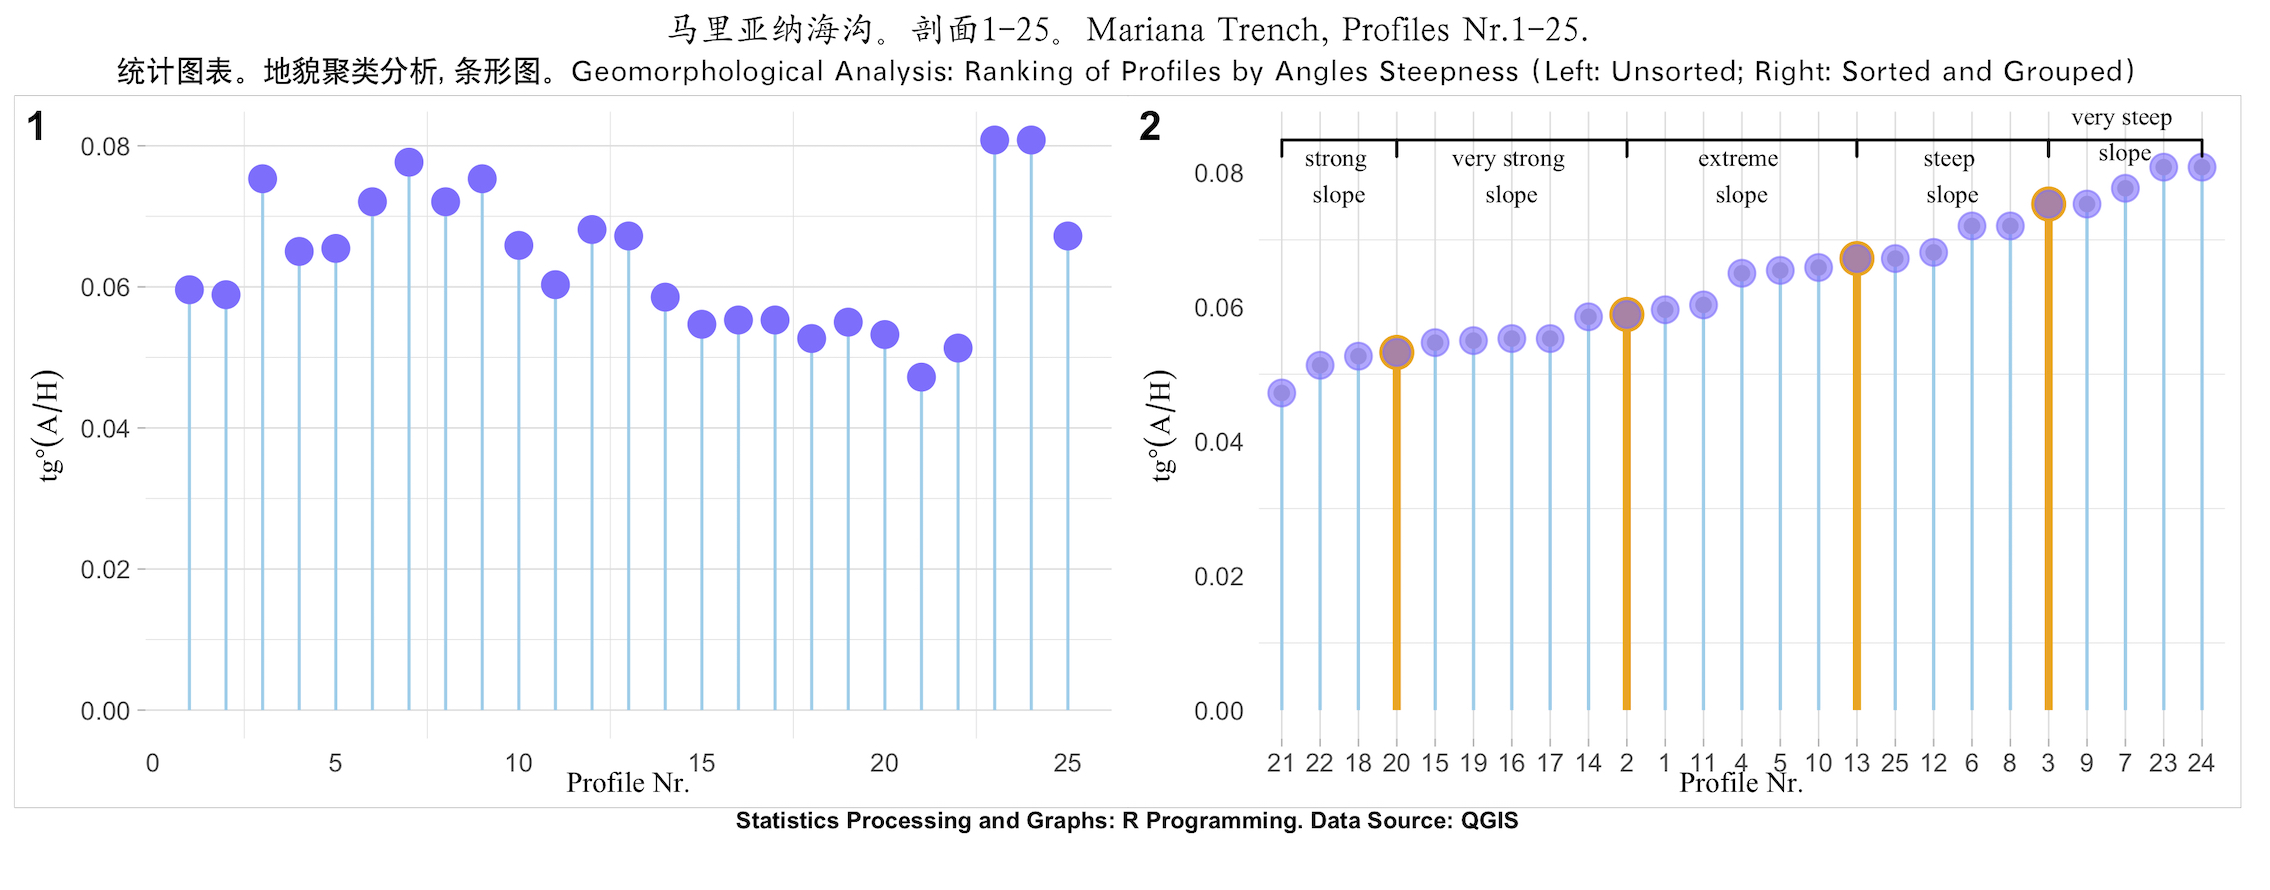
\includegraphics[width=11cm]{Fig-3-9.jpg}
	\caption{Steepness angles by the bathymetric profiles 1:25 of the Mariana Trench: unsorted (left); sorted and grouped (right).}
\end{figure}		
\end{frame}

\begin{frame}[fragile]\frametitle{R code for highlighted groups by steepness angles by libraries \{ggsignif\} and \{tidyverse\}: Part-1}
\begin{lstlisting}[language=R]
# Part-1. Prepare data frame 
	# step-1. read in table. create initial data frame, clean up from the NA
MDepths <- read.csv("Morphology.csv", header=TRUE, sep = ",")
MDF <- na.omit(MDepths) 
row.has.na <- apply(MDF, 1, function(x){any(is.na(x))}) 
sum(row.has.na) 
head(MDF)
	# step-2  Create short data from 3 values
data<- data.frame(x = MDF$profile, y = MDF$tg_angle)
p_unsort<- ggplot(data, aes(x=x, y=y)) +
	geom_segment( aes(x=x, xend=x, y=0, yend=y), color="skyblue", size=0.5) +
	geom_point( color="slateblue1", size=4) +
	coord_flip() +
	theme_light() +
	theme(panel.grid.major.x = element_blank(),
	panel.border = element_blank(),
	axis.ticks.x = element_blank(),
	axis.title.y = element_text(margin = margin(t = 20, r = 3), family = "Times New Roman", face = 1, size = 10),
	axis.title.x = element_text(family = "Times New Roman", face = 1, size = 10, margin = margin(t = .2)),
	) +
	xlab("Profile Nr.") +
	ylab(expression(tg*degree*(A/H)))
p_unsort
\end{lstlisting}		
\end{frame}

\begin{frame}[fragile]\frametitle{R code for highlighted groups by steepness angles by libraries \{ggsignif\} and \{tidyverse\}: Part-2}
\begin{lstlisting}[language=R]
	# step-3. Reorder
p_sort <- data %>%
	arrange(y) %>%
	mutate(x=factor(x,x)) %>%
	ggplot( aes(x=x, y=y)) +
	geom_segment( aes(x=x, xend=x, y=0, yend=y), color="skyblue", size=0.5) +
	geom_segment( aes(x=x, xend=x, y=0, yend=y ), color=ifelse(data$x %in% c("4", "10", "16", "21"), "orange", "skyblue"), size=ifelse(data$x %in% c("4", "10", "16", "21"), 1.3, 0.5) ) +
	geom_point( color=ifelse(data$x %in% c("4", "10", "16", "21"), "orange", "grey"), size=ifelse(data$x %in% c("4", "10", "16", "21"),  5,  2) ) +
	geom_point( color="slateblue1", size=4, alpha=0.6) +
	geom_signif(comparisons = list(c("21", "20")), annotation="strong \nslope", map_signif_level=TRUE, vjust = 1.3, textsize = 3.0, family = "Times New Roman") +
	geom_signif(comparisons = list(c("20", "2")), annotation="very strong \nslope", map_signif_level=TRUE, vjust = 1.3, textsize = 3.0, family = "Times New Roman") +
	geom_signif(comparisons = list(c("2", "13")), annotation="extreme \nslope", map_signif_level=TRUE, vjust = 1.3, textsize = 3.0, family = "Times New Roman") +
	geom_signif(comparisons = list(c("13", "3")), annotation="steep \nslope", map_signif_level=TRUE, vjust = 1.3, textsize = 3.0, family = "Times New Roman") +
	geom_signif(comparisons = list(c("3", "24")), annotation="very steep \nslope", map_signif_level=TRUE, vjust = 0.5, textsize = 3.0, family = "Times New Roman") +
	theme_light() +
 #   coord_flip() +
\end{lstlisting}		
\end{frame}

\begin{frame}[fragile,shrink=20]\frametitle{R code for highlighted groups by steepness angles by libraries \{ggsignif\} and \{tidyverse\}: Part-3}
\begin{lstlisting}[language=R]
    theme(panel.grid.major.y = element_blank(), 
	panel.border = element_blank(),axis.ticks.y = element_blank(),
	axis.title.y = element_text(margin = margin(t = 20, r = 3), family = "Times New Roman", face = 1, size = 10),
	axis.title.x = element_text(family = "Times New Roman", face = 1, size = 10, margin = margin(t = .2)),
	) +
	xlab("Profile Nr.") +
	ylab(expression(tg*degree*(A/H)))
 p_sort
	# step-4 add both plots on one layout
 figure <-plot_grid(p_unsort, p_sort, labels = c("1", "2"), ncol = 2, nrow = 1)
 figure
	# step-5. add common title, subtitle, overall design and lower subscript
Ranking <- figure +						
	labs(title="Mariana Trench, Profiles Nr.1-25.", 
	subtitle = "Geomorphological Analysis: Ranking of Profiles by Angle Steepness (Left: Unsorted; Right: Sorted and Grouped)",
	caption = "Statistics Processing and Graphs: R Programming. Data Source: QGIS") +
theme(
	plot.margin = margin(5, 10, 20, 5),
	plot.title = element_text(margin = margin(t = 0, r = 20, b = 5, l = 0), family = "Kai", face = "bold", size = 12), 
	plot.subtitle = element_text(margin = margin(t = 0, r = 20, b = 4, l = 0), family = "Hei", face = "bold", size = 10), 
	plot.caption = element_text(face = 2, size = 8),
	panel.background=ggplot2::element_rect(fill = "white"),
	legend.justification = "bottom", legend.position = "bottom",
	legend.box.just = "right", legend.direction = "horizontal",
	legend.box = "horizontal", legend.box.background = element_rect(colour = "honeydew4",size=0.2),
	legend.background = element_rect(fill = "white"),
	legend.key.width = unit(1,"cm"), legend.key.height = unit(.5,"cm"),
	legend.spacing.x = unit(.2,"cm"), legend.spacing.y = unit(.1,"cm"),
	legend.text = element_text(colour="black", size=6, face=1),
	legend.title = element_text(colour="black", size=6, face=1))
Ranking
\end{lstlisting}
\end{frame}

\begin{frame}\frametitle{Compositional Charts (a.k.a. Waffle Charts)}
\begin{figure}[H]
	\centering
		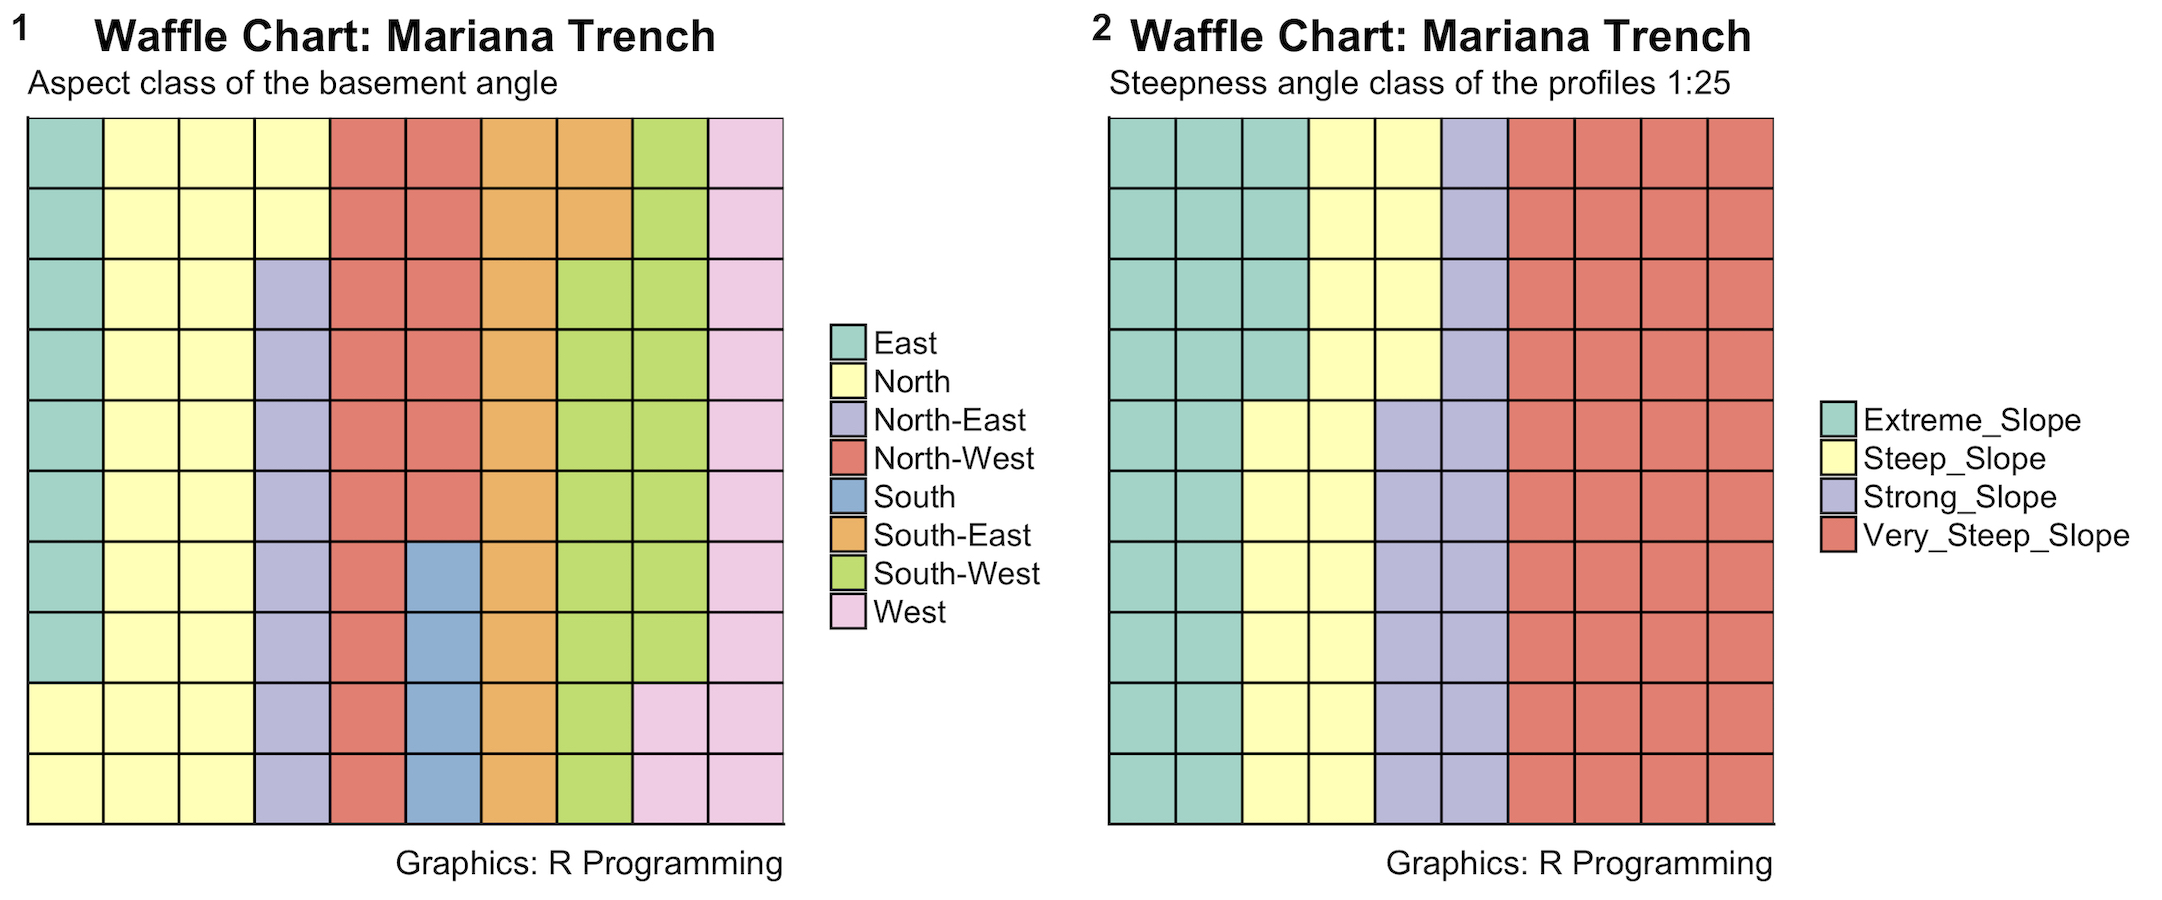
\includegraphics[width=11cm]{Fig-3-10.jpg}
	\caption{Compositional charts of the determinants variations}
\end{figure}		
\end{frame}

\begin{frame}[fragile,shrink=10]\frametitle{R code for 'waffle' plot by library \{ggplot2\} (1)}
\begin{lstlisting}[language=R]
	# step-1 load table with data. create data frame
MDF <- read.csv("Morphology.csv", header=TRUE, sep = ",")
MDF <- na.omit(MDF) 
row.has.na <- apply(MDF, 1, function(x){any(is.na(x))}) 
sum(row.has.na) 
head(MDF)
	# step-2. variant-1: aspect class. 
var <- MDF$aspect_class  # This is a categorical data. Here: 8 aspect classes
nrows <- 10
df <- expand.grid(y = 1:nrows, x = 1:nrows) # set up square 10*10
categ_table <- round(table(var) * ((nrows*nrows)/(length(var)))) # set up table with categorial values
categ_table
df$category <- factor(rep(names(categ_table), categ_table)) # names to be shown in a legend
# note: if sum(categ_table) is not 100 (i.e. nrows^2), it will need adjustment to make the sum to 100.
	# step-3. Plot 'waffle' diagram
wa<- ggplot(df, aes(x = x, y = y, fill = category)) +
	geom_tile(color = "black", size = 0.5) +
        scale_x_continuous(expand = c(0, 0)) +
        scale_y_continuous(expand = c(0, 0), trans = 'reverse') +
        scale_fill_brewer(palette = "Set3") +
        labs(title="Waffle Chart: Mariana Trench", subtitle="Aspect class of the basement angle",
        caption="Graphics: R Programming")  + 
        theme( plot.title = element_text(size = rel(1.2)),
        axis.text = element_blank(),
        axis.title = element_blank(),
        axis.ticks = element_blank(),
        legend.title = element_blank(),
        legend.position = "right")
wa
\end{lstlisting}
\end{frame}

\begin{frame}[fragile]\frametitle{R code for 'waffle' plot by library \{ggplot2\} (2)}
\begin{lstlisting}[language=R]
	# step-4. variant-2: slope steepness class. create table and load data.
var <- MDF$morph_class  #  the categorical data: slope steepness class
nrows <- 10
df <- expand.grid(y = 1:nrows, x = 1:nrows) # задаем квадрат 10*10
categ_table <- round(table(var) * ((nrows*nrows)/(length(var)))) # set up table with categorial values
categ_table
df$category <- factor(rep(names(categ_table), categ_table)) # names to be shown in a legend
	# step-5. Plot waffle diagram by steepness
ws<- ggplot(df, aes(x = x, y = y, fill = category)) + 
        geom_tile(color = "black", size = 0.5) +
        scale_x_continuous(expand = c(0, 0)) +
        scale_y_continuous(expand = c(0, 0), trans = 'reverse') +
        scale_fill_brewer(palette = "Set3") +
        labs(title="Waffle Chart: Mariana Trench", subtitle="Steepness angle class of the profiles 1:25",
        caption="Graphics: R Programming")  + 
        theme( plot.title = element_text(size = rel(1.2)),
        axis.text = element_blank(),
        axis.title = element_blank(),
        axis.ticks = element_blank(),
        legend.title = element_blank(),
        legend.position = "right")
ws
	#step-6. combine both waffles on one plot
figure <-plot_grid(wa, ws, labels = c("1", "2"), ncol = 2, nrow = 1)
figure
\end{lstlisting}
\end{frame}

\begin{frame}\frametitle{R plot for correlation ellipses using library\{ellipse\}}
\begin{figure}[H]
	\centering
		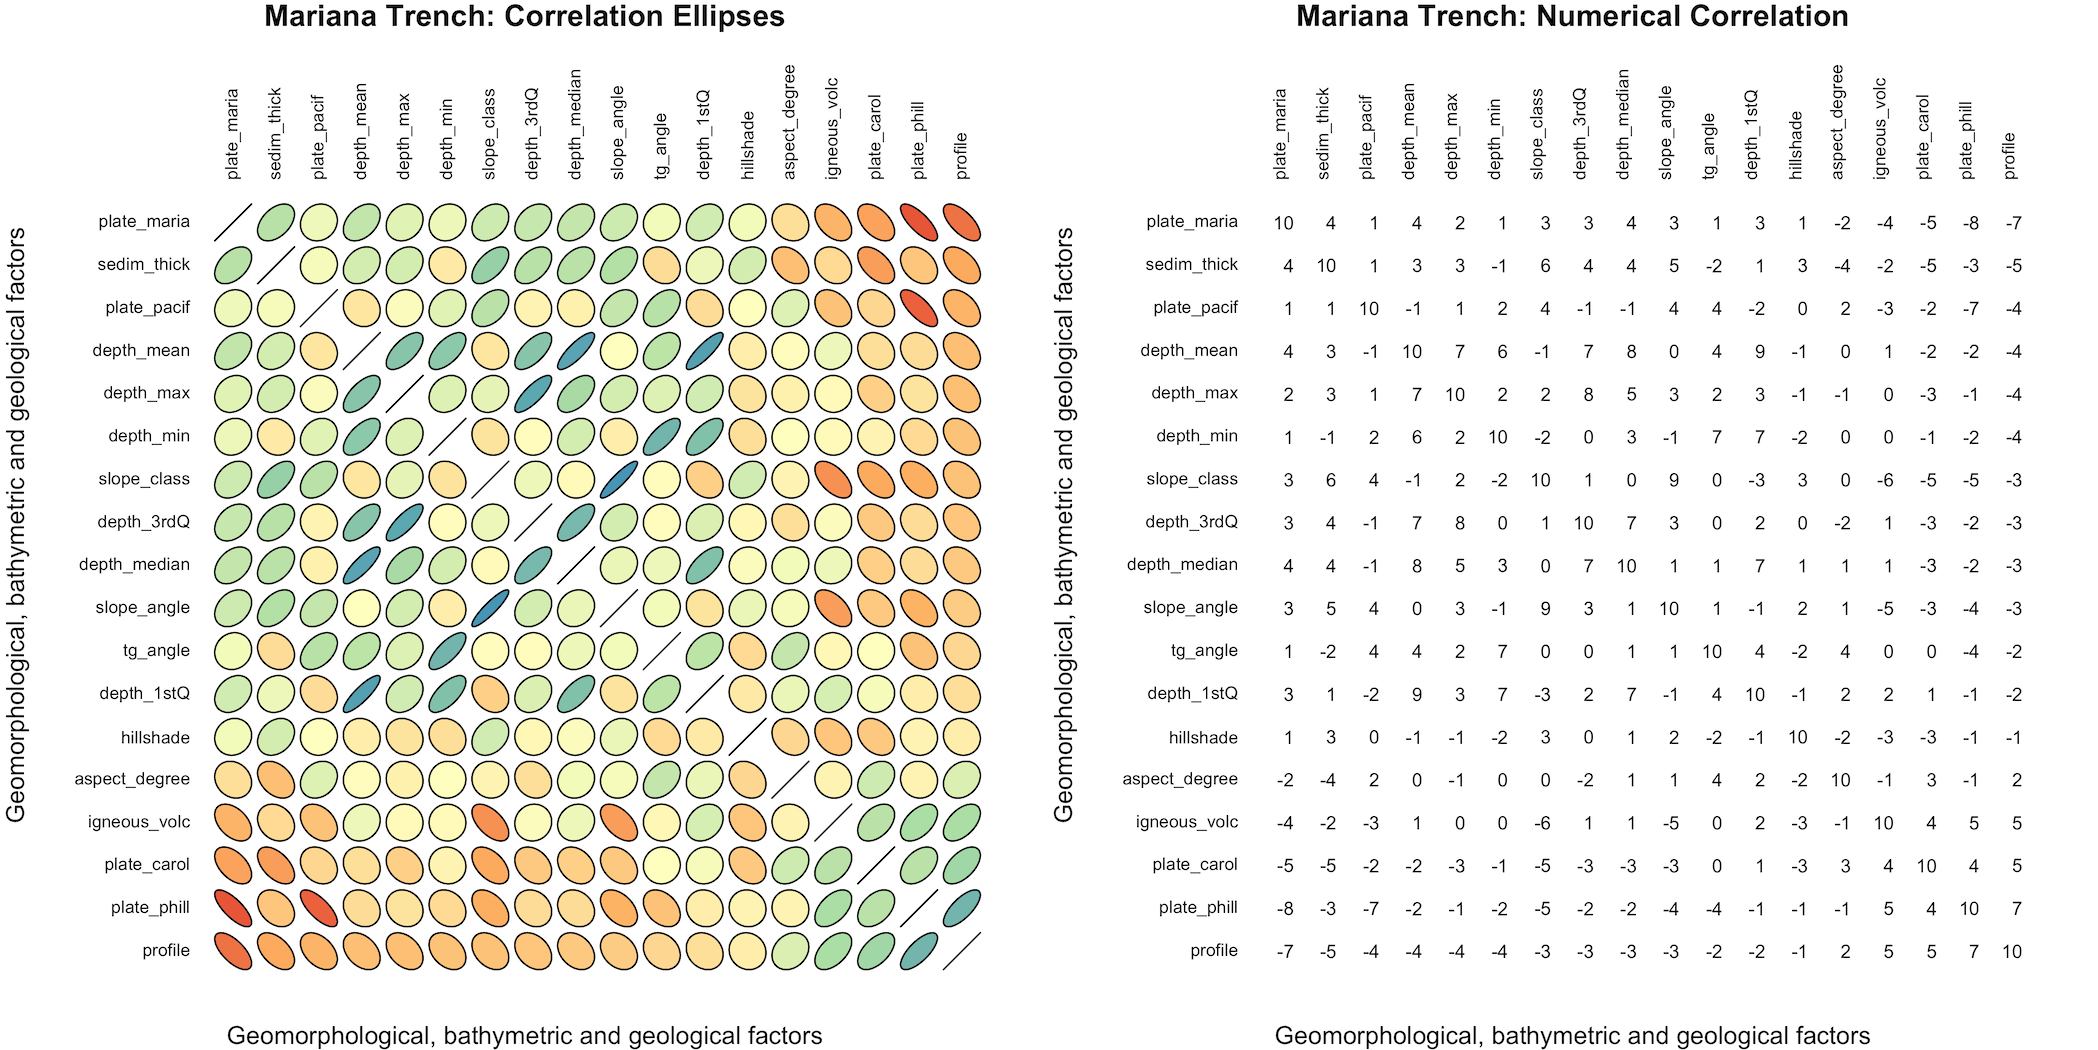
\includegraphics[width=11cm]{Fig-4-1.jpg}\caption{Correlation ellipses. Left: ellipses view, right: numeric view, R.}
\end{figure}		
\end{frame}

\begin{frame}[fragile]\frametitle{R code plot correlation ellipses using library\{ellipse\}}
\begin{lstlisting}[language=R]
	# step-1. read in table. create data frame.
MDF <- read.csv("Morphology.csv", header=TRUE, sep = ",")
MDF <- na.omit(MDF) 
row.has.na <- apply(MDF, 1, function(x){any(is.na(x))}) 
sum(row.has.na) 
head(MDF)
	# step-2. plot correlation ellipses using libraries (ellipse) and (RColorBrewer)
data=cor(MDF)
	# Build a panel of 100 colors with Rcolor Brewer
my_colors <- brewer.pal(5, "Spectral")
my_colors=colorRampPalette(my_colors)(100)
	# step-3. Order correlation matrix
ord <- order(data[1, ])
data_ord = data[ord, ord]
	# step-4. variant-1 correlation ellipses
plotcorr(data_ord , col=my_colors[data_ord*50+50] , mar=c(1,1,1,1), 
	outline = TRUE, numbers = FALSE,
	main = "Mariana Trench: Correlation Ellipses", 
	xlab = "Geomorphological, bathymetric and geological factors", 
	ylab = "Geomorphological, bathymetric and geological factors", 
	cex.lab = 0.7)
	# step-5. variant-2 correlation numbers	
plotcorr(data_ord , col=my_colors[data_ord*50+50] , mar=c(1,1,1,1), 
	outline = TRUE, numbers = TRUE,
	main = "Mariana Trench: Numerical Correlation", 
	xlab = "Geomorphological, bathymetric and geological factors", 
	ylab = "Geomorphological, bathymetric and geological factors", 
	cex.lab = 0.7)
\end{lstlisting}
\end{frame}

\begin{frame}\frametitle{Scatterplot matrices}
\begin{figure}[H]
	\centering
		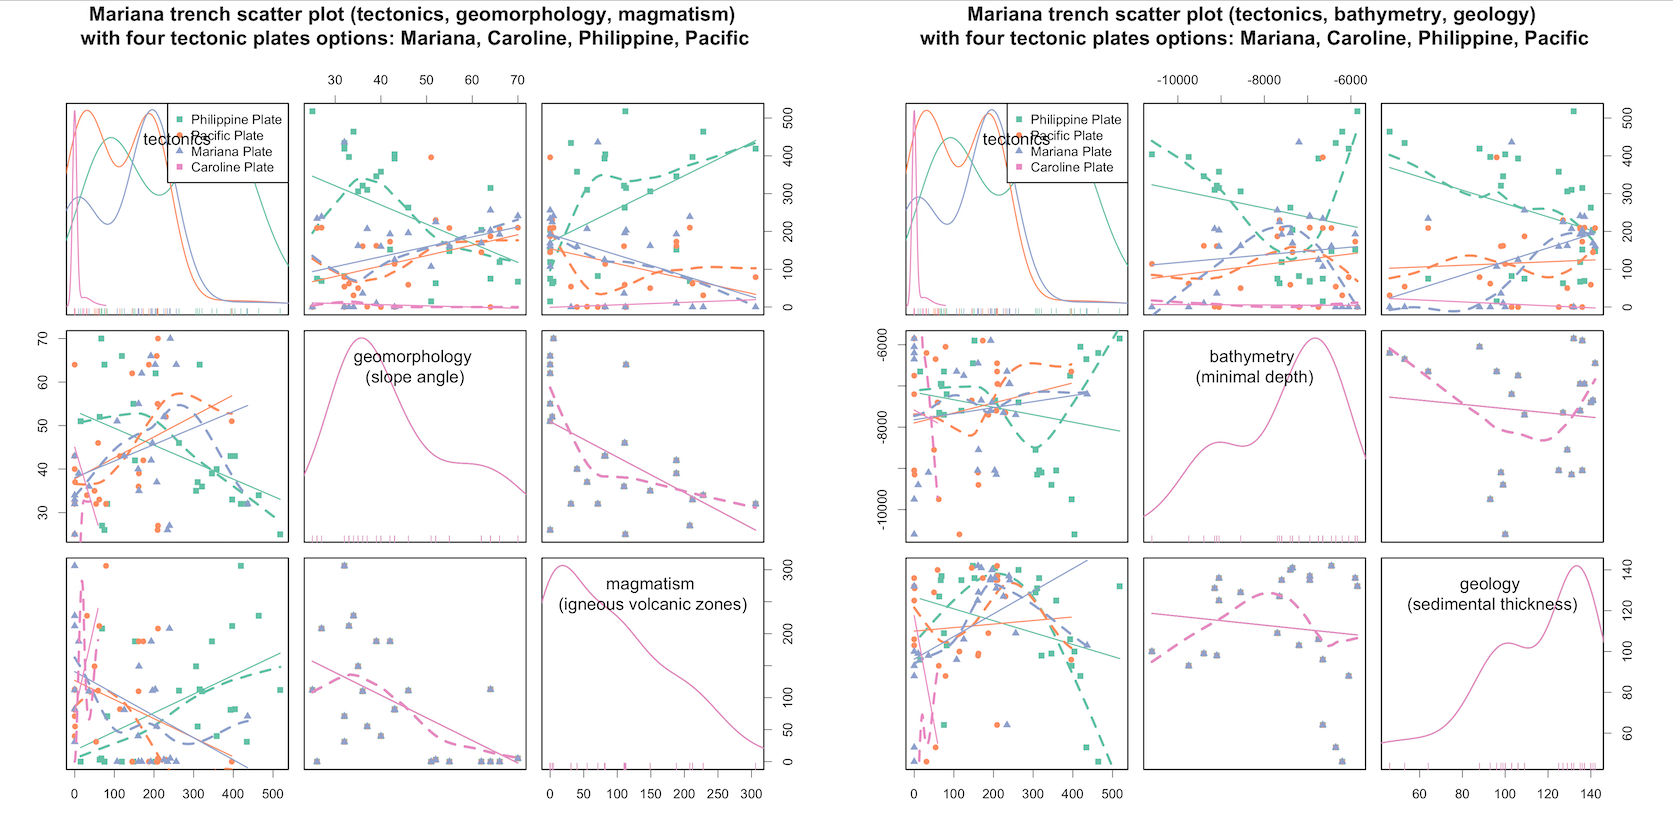
\includegraphics[width=11cm]{Fig-4-4.jpg}
	\caption{Scatterplot matrices}
\end{figure}		
\end{frame}

\begin{frame}[fragile]\frametitle{R code for diagonal scatterplot matrices\\ \{car\} library: Part 1}
Steps 1-4. 
\begin{lstlisting}[language=R]
library(car)
library(RColorBrewer)
# Part 1: create data.frame
	# step-1. read in table. build data frame
MDF <- read.csv("Morphology.csv", header=TRUE, sep = ",")
MDF <- na.omit(MDF) 
row.has.na <- apply(MDF, 1, function(x){any(is.na(x))}) 
sum(row.has.na) 
head(MDF) 
	# step-2. merge values of 4 tectonic plates into one category
MDFT = melt(setDT(MDF), measure = patterns("^plate"), value.name = c("tectonics"))
head(MDFT)
levels(MDFT$variable) = c("Philippine Plate" , "Pacific Plate", "Mariana Plate", "Caroline Plate") # rename values
head(MDFT)
	# step-3. read data frame into object 'data'
data= MDFT 
	# step-4. set up colors Set2 by category 'tectonics'
my_colors <- brewer.pal(nlevels(as.factor(data$variable)), "Set2")
\end{lstlisting}		
\end{frame}

\begin{frame}[fragile]\frametitle{R code for diagonal scatterplot matrices\\ \{car\} library: Part 2}
Steps 5-7.
\begin{lstlisting}[language=R]
# Part-2. Plotting
	# step-5. Variant-1: tectonics + slope angle + igneous volcanic zones
scatterplotMatrix(~ tectonics + slope_angle + igneous_volc | variable, data=data ,  	
	smoother="", col=my_colors , smoother.args=list(col="grey") ,  
	regLine = list(method=lm, lty=1, lwd=1),
	lwd=0.5, pch=c(15,16,17) , 
	main="Mariana trench scatter plot (tectonics, geomorphology, magmatism) \nwith four tectonic plates options: Mariana, Caroline, Philippine, Pacific", 
	cex=1.0, cex.axis = 1.0, # cex.axis, font of legend
	legend = TRUE, cex.labels =1.3, cex.main = 1.0, ellipse=F,
	var.labels = c("tectonics", "geomorphology \n(slope angle)", "magmatism \n(igneous volcanic zones)")
	)
	# step-6. Variant-2: depths + sediments + igneous volcanic zones
scatterplotMatrix(~ tectonics + Min + sedim_thick | variable, data=data , 
	smoother="", col=my_colors , smoother.args=list(col="grey") ,  
	regLine = list(method=lm, lty=1, lwd=1),
	lwd=0.5, pch=c(15,16,17) , 
	main="Mariana trench scatter plot (tectonics, bathymetry, geology) \nwith four tectonic plates options: Mariana, Caroline, Philippine, Pacific", 
	cex=1.0, cex.axis = 1.0, # cex.axis, font of legend
	legend = TRUE, cex.labels =1.3, cex.main = 1.0, ellipse=F,
	var.labels = c("tectonics", "bathymetry \n(minimal depth)", "geology \n(sedimental thickness)")
	)
	# step-7. plotting
plot(data , pch=1 , cex=0.3 , col=rgb(0.5, 0.8, 0.9, 0.7))
\end{lstlisting}		
\end{frame}

% ----------------------------------------------------------------------------
% *** END: Workflow >>>
% ----------------------------------------------------------------------------

% ----------------------------------------------------------------------------
% *** START: Results <<<
% ----------------------------------------------------------------------------

\section{Results}
\begin{frame}\frametitle{Results - I. Bathymetry: north, profiles 1-19}
Statistical analysis revealed following findings:
\begin{itemize}
    \item The major depth observation points of the Mariana Trench are located in between the -3000 and -5000 m.
    \item The widths of the confidence intervals are expanding rapidly by the profiles 12 to 15 thus indicating on the large amplitude of the depths variations in this part of the Mariana Trench.
    \item The profile depths are affected by the local geographic features caused by the location on 4 tectonic plates with varying environmental conditions.
    \item Conversely, profiles from 1 to 16 have gradual decrease in absolute depths, which can be noted in outliers sample location. 
    \item A slight increase in absolute depths of the profiles \textnumero \space 4-8. 
\end{itemize}
\end{frame}
	
\begin{frame}\frametitle{Results - II. Bathymetry: south, profiles 20-25}
Summaries of the variations of the local polynomial regression of the bathymetric depths of the measured samples are presented. \begin{itemize}
    \item The maximal depths reach up to -10000 in the current dataset: profiles \textnumero 20, 21, 22 crossing mostly Philippine tectonic plate (t.p.).
    \item The widths of the confidence intervals expand rapidly by the profiles 19 to 22 indicating on the large amplitude of the depths variations in this part of the trench.
    \item Decrease of depth: profiles \textnumero 23, 24, 25, Caroline t.p.
    \item Profiles \textnumero 23 and 24 demonstrate the deepest depth values. 
    \item The absolute depths in the profiles 22 to 25 on the Caroline t.p. become shallower than those on Philippine and Pacific t.p.
    \item The majority of the observation points: Pacific and Philippine t.p., following by Mariana t.p.. Caroline t.p. only covers a few points. 
    \item Variability in the geological factors of the underlying t.p. triggers changes in bathymetric settings
\end{itemize}
\end{frame}	

\begin{frame}\frametitle{Results - III. Sediment thickness}
The sediment thickness changes notably both within the trench by profiles (1:25) and between four tectonic plates that Mariana Trench crosses: Philippine, Pacific, Mariana and Caroline. Since the tectonic properties and attribute values of them are not identical. The comparative analysis of how the data vary across four distinctive plates revealed that the middle part of the Mariana Trench (profiles: 14 up to 17) has roughly equal proportions of the sediment thickness layer, which indicates that
    	\begin{itemize}
    		 \item spatial locations and distributions of the volcanic areas and slope angle of the ocean trench are closely interrelated; 
		 \item geographic distributions of the volcanic areas and steepness of the slope angles of the ocean trench affect sedimental thickness. 
	\end{itemize}
\end{frame}
	
\begin{frame}\frametitle{Results - IV. Angle steepness (1)}
Analysis of the angle steepness of the cross-section profiles along Mariana Trench revealed following findings:
    	\begin{itemize}
		 \item The major trend of the trench angles located on the Pacific plate has downward general line trend. 
		 \item The Philippine tectonic plate, on the contrary, has a minimal peak by profiles \textnumero \space 14-21, and then moving upwards. 
		 \item The highest value for the trench angle steepness is within Caroline t.p. 
		 \item Mariana plate has the highest density of depth distribution values, followed by the Philippine plate, then Pacific and Caroline, respectively. 
		 \item From two multiple panel graphs by groups one can compare the slope angles and depth distributions by tectonic plates. 
	\end{itemize}
\end{frame}

\begin{frame}\frametitle{Results - V. Angle steepness (2)}	

	\begin{itemize}
		 \item A bunch of bathymetric cross-section profiles form a cluster groups with similar geomorphic properties divided into five groups over the study area. 
		 \item Thus, profiles: 21, 22, 18 and 20 have all “strong slope” tg\degree angle degree, which is an average of 0.05. 
		 \item Similarly, profiles: 15, 19, 16, 17, 14 and 2, belonging to class “very strong slope”, have an tg\degree angle of 0.057 to 0.058 (Figure 19). 
		 \item When compared with third group in the study area, such as class “extreme slope” (profiles: 1, 11, 4, 5, 10 and 13), the average slope tg\degree angle fluctuating from 0.060 to 0.070. 
		 \item The fourth group is class “steep slope” (profiles: 25, 12, 6, 8 3) with a slope tg\degree angle values from 0.070 to 0.075. 
		 \item Finally, the last group is notable for the highest steepness (profiles: 9, 7, 23, 24), with average slope tg\degree angle degree up to 0.079. 
	\end{itemize}		 
\end{frame}

% ----------------------------------------------------------------------------
% *** END: Results >>>
% ----------------------------------------------------------------------------

% ----------------------------------------------------------------------------
% *** START: Conclusion <<<
% ----------------------------------------------------------------------------

\section{Conclusion}
\begin{frame}\frametitle{Conclusion}

	\begin{exampleblock}{Impact Factors}
The slope steepness is generally related to the slab subduction (tectonic settings) in the particular area, but may also be associated with other factors: topography, submarine volcanism, geology, oceanology.
	\end{exampleblock}
	
	\begin{exampleblock}{Enevenness} As a result of the undertaken study, a strong spatial geomorphic unevenness of the Mariana Trench has been revealed: the middle part (profiles: 14 up to 17) has very strong slopes and roughly equal proportions of the sediment thickness layer, while other parts differ.\\ Five unique regions across the trench length have been classified.
	\end{exampleblock}
	
	\begin{alertblock}{Applied statistics using R}
	The impact of various factors (oceanology, geology, submarine volcanism, tectonics) affecting structure and geomorphology of the Mariana Trench were studied by means of R programming language.
	\end{alertblock}
\end{frame}

\begin{frame}\frametitle{Impact Factors}
\begin{figure}[H]
	\centering
		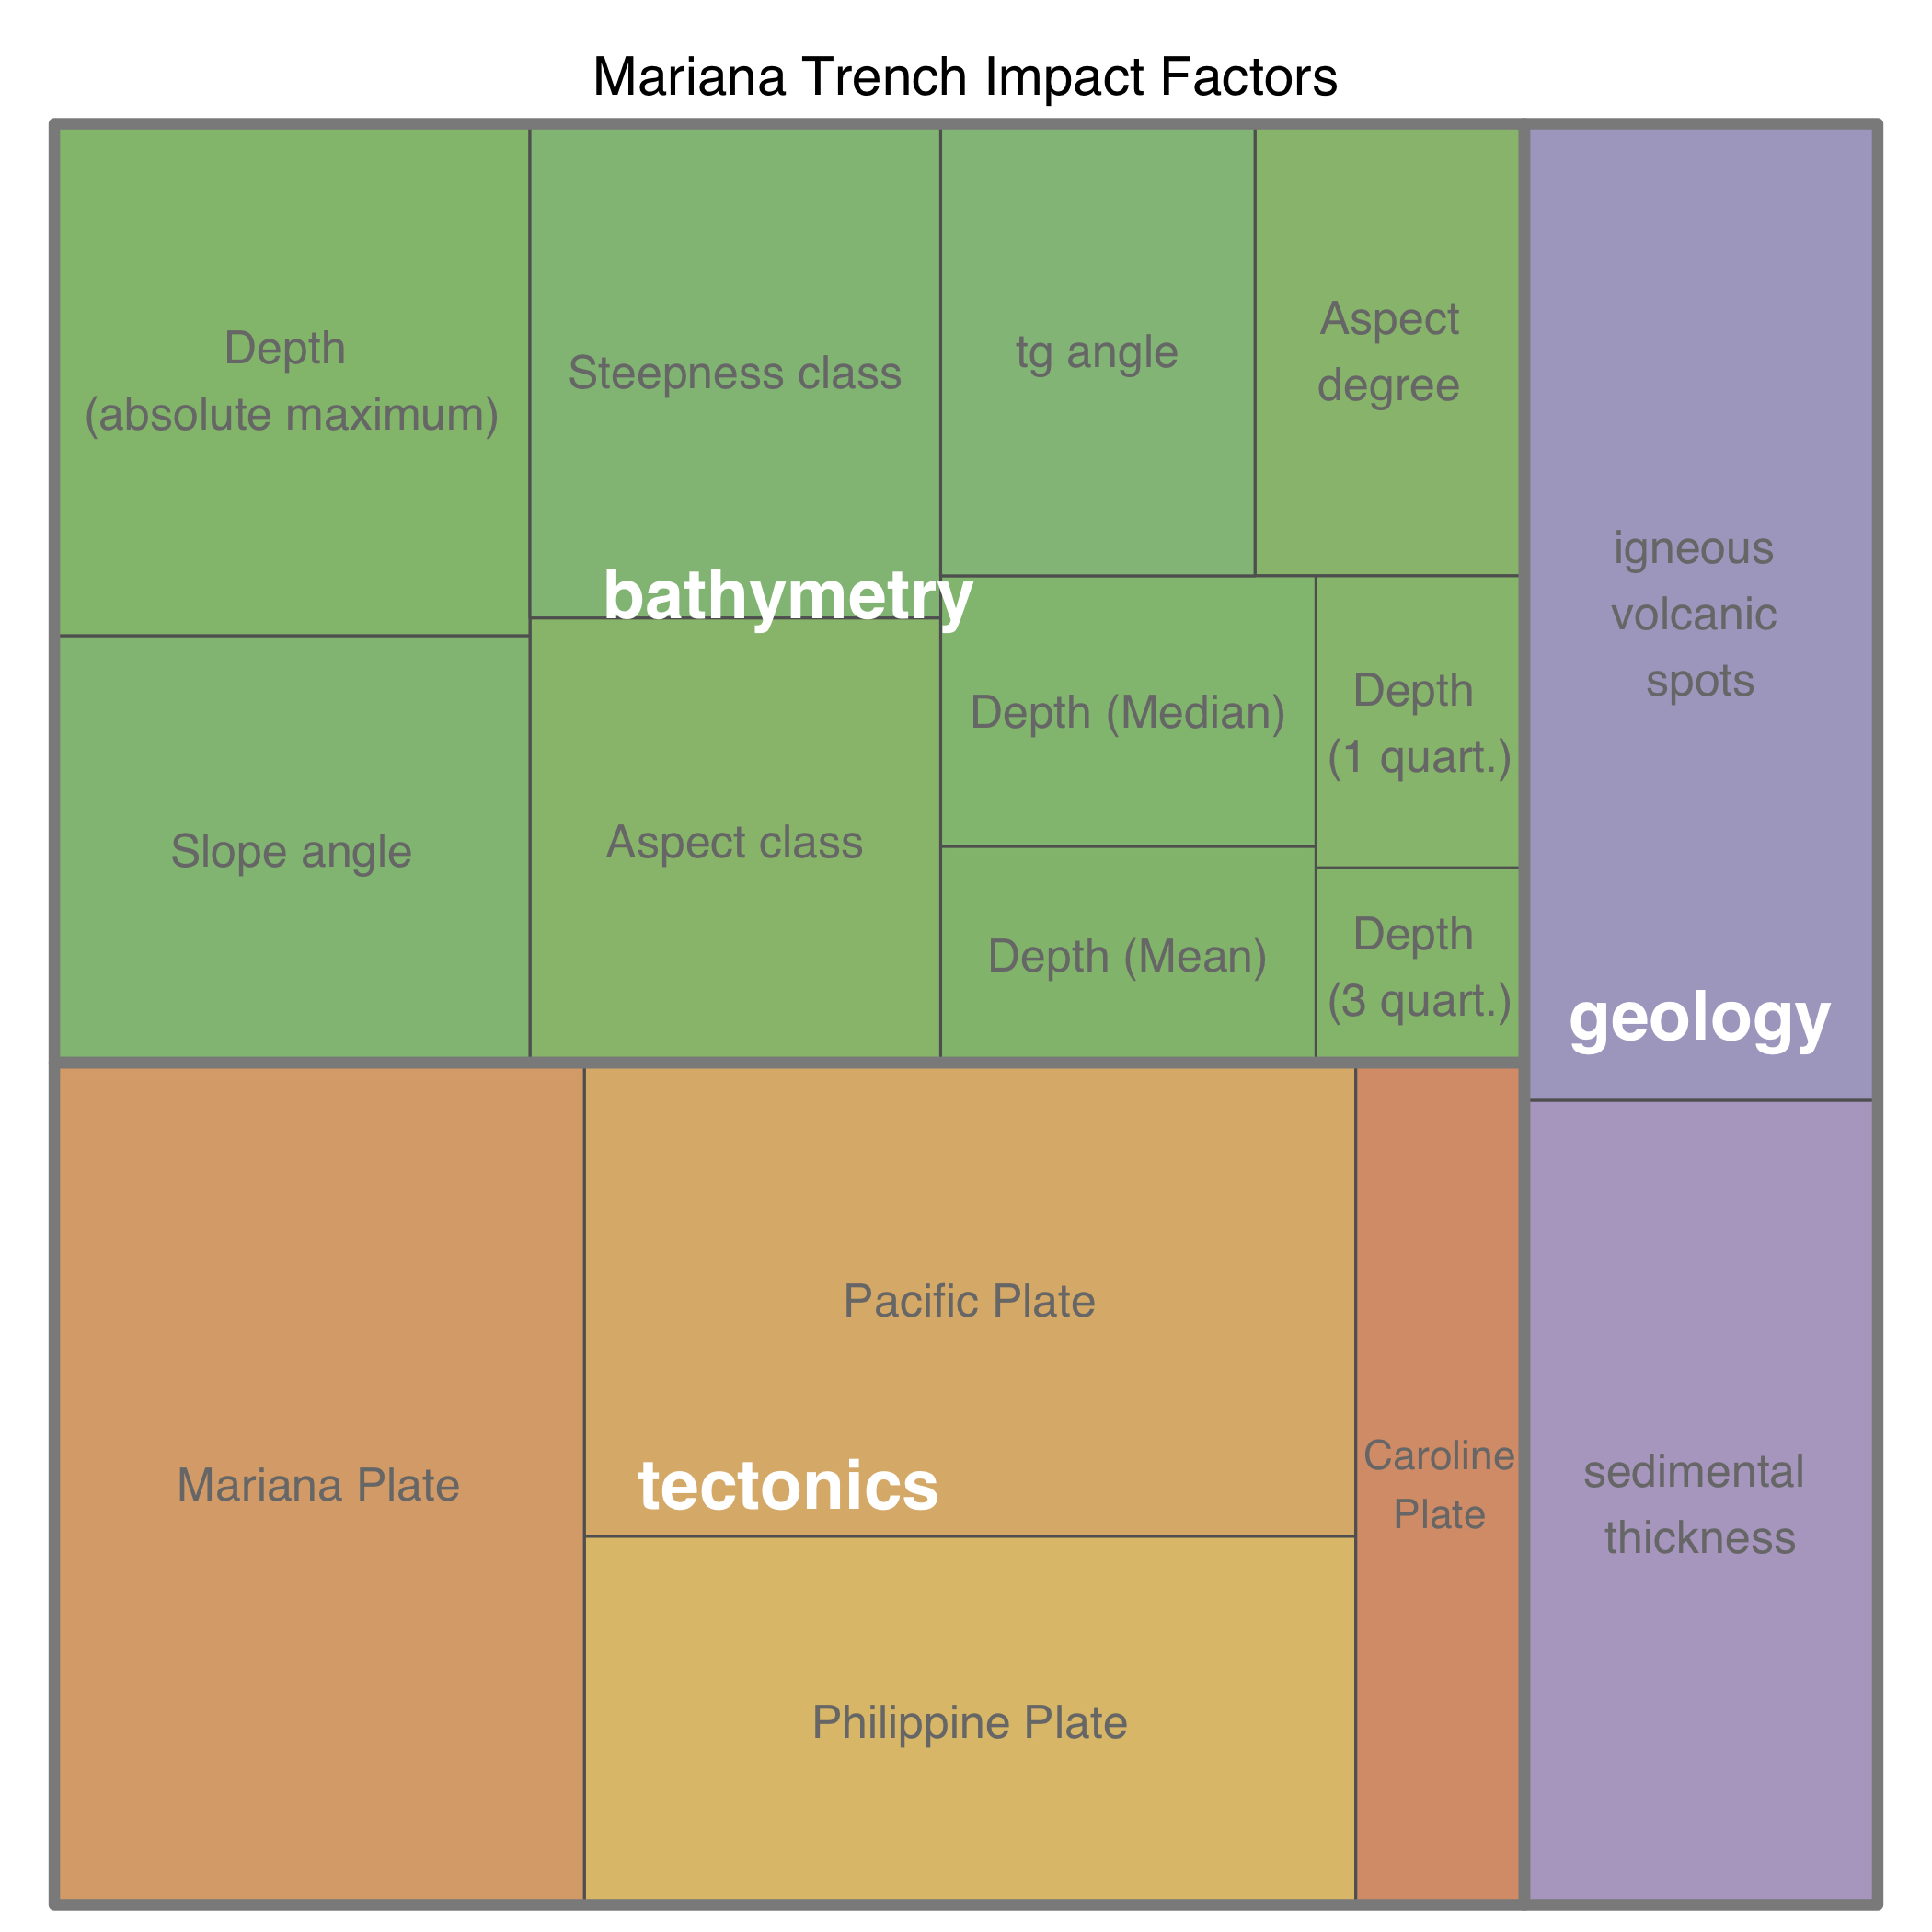
\includegraphics[width=6cm]{Fig-5-1.jpg}\caption{Treemap for impact factors affecting Mariana Trench formation, R visualization.}
\end{figure}		
\end{frame}

\begin{frame}[fragile]\frametitle{R code for treemap by library \{treemap\}}
\begin{lstlisting}[language=R]
library(treemap)
	# step-1. Create a dataset
group=c(rep("tectonics",4),rep("bathymetry",10),rep("geology",2))
subgroup=paste(c("Mariana Plate", "Philippine Plate", "Pacific Plate", "Caroline Plate", 
		"Depth \n(absolute maximum)", "Slope angle", "Aspect degree", "Depth (Mean)", "Depth (Median)", "Aspect class", "Steepness class", "Depth \n(1 quart.)", "Depth \n(3 quart.)", "tg angle", 
		"sedimental \nthickness", "igneous \nvolcanic \nspots"))
value=c(22,14,18,7,12,10,6,4,5,9,10,3,2,7,14,17)
data=data.frame(group,subgroup,value)
	# step-2. Plot treemap
treemap(data,
	title = "Mariana Trench Impact Factors",
	index=c("group","subgroup"),
	palette="Accent",
	vSize="value",
	type="index" ,
	fontsize.labels=c(18,12),# size of labels per level of aggregation: group, subgroup, subsubgroups
	fontcolor.labels=c("white","gray40"),
	fontface.labels=c(2,1),# Fonts: 1,2,3,4 for normal, bold, italic, bold-italic
	bg.labels=c("transparent"),# Background color of labels
	align.labels=list(c("center", "center"), c("center", "center")),
	overlap.labels=0.9,
	inflate.labels=F,# If true, labels are bigger when rectangle is bigger.
	border.col=c("gray48","gray30"),# Color of borders of groups, of subgroups
	border.lwds=c(4,1)
)
\end{lstlisting}
\end{frame}

\begin{frame}\frametitle{Euler-Venn diagrams: 4 and 6 petals}
\begin{figure}[H]
	\centering
		\subfloat {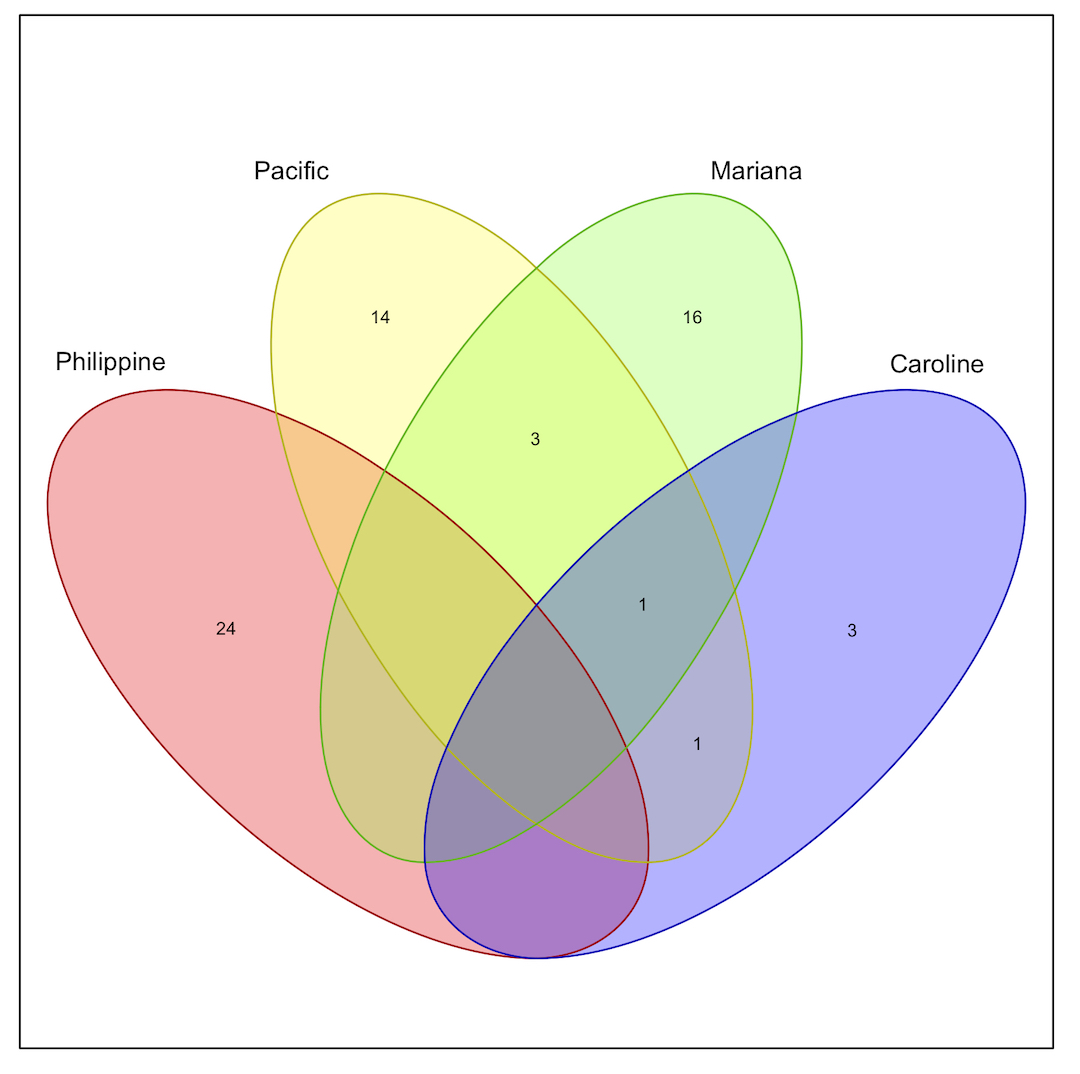
\includegraphics[width=5cm]{Fig-5-2a.jpg}}
			\hspace{3mm}
		\subfloat {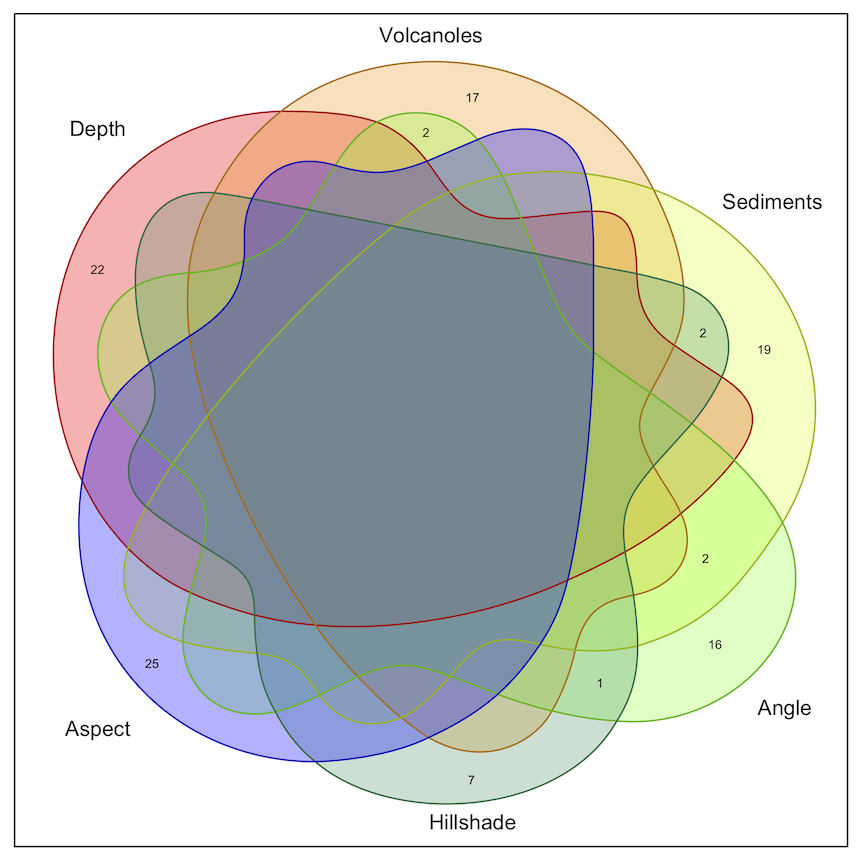
\includegraphics[width=5cm]{Fig-5-2b.jpg}}
			\hspace{3mm}
	\caption{Possible correlations of the impact factors affecting Mariana Trench. \\Left: four tectonic plates. Right: environmental factors}.
\end{figure}
\end{frame}

\begin{frame}\frametitle{Euler-Venn diagrams: 7 petals}
\begin{figure}[H]
	\centering
		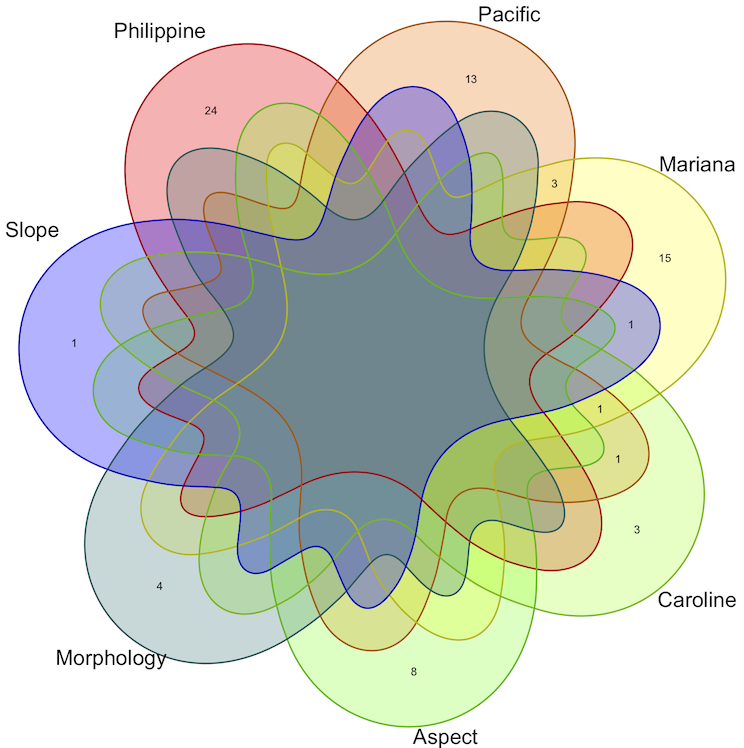
\includegraphics[width=6.5cm]{Fig-5-2c.jpg}\caption{Correlations of the impact factors affecting Mariana Trench, R}.
\end{figure}		
\end{frame}

\begin{frame}[fragile,shrink=10]\frametitle{R code for Euler-Venn Diagram (logical correlation of objects) using \{venn\} library}
\begin{lstlisting}[language=R]
# Part-1. Prepare dataframe 
	# step-1. Read table. Clean up NA
MDepths <- read.csv("Morphology.csv", header=TRUE, sep = ",")
MDF <- na.omit(MDepths) 
row.has.na <- apply(MDF, 1, function(x){any(is.na(x))}) 
sum(row.has.na) 
head(MDF) 
# Part-2. Create Euler-Venn Diagram: 3 cases. 
library(venn)
	# step-2. 
 		# case-1. Morphology and tectonic plates
	x <- list(Philippine = MDF$plate_phill, Pacific = MDF$plate_pacif, 
	Mariana = MDF$plate_maria, Caroline = MDF$plate_carol, 
	Aspect = MDF$aspect_class, 
	Morphology = MDF$morph_class, Slope = MDF$slope_class)
	venn(x, ilabels = TRUE, col = "navyblue", zcolor = "style")
		# case-2. tectonics plates
	xp <- list(Philippine = MDF$plate_phill, Pacific = MDF$plate_pacif, 
	Mariana = MDF$plate_maria, Caroline = MDF$plate_carol)
	venn(xp, ilabels = TRUE, ellipse = TRUE, col = "navyblue", 
	zcolor = "style")
		# case-3. Geomorphic parameters
	x3 <- list(Depth = MDF$Min, Volcanoles = MDF$igneous_volc, 
	Sediments = MDF$sedim_thick, 
	Angle = MDF$slope_angle, Hillshade = MDF$hillshade, 
	Aspect = MDF$aspect_degree)
	venn(x3, ilabels = TRUE, col = "navyblue", zcolor = "style")
\end{lstlisting}
\end{frame}

% ----------------------------------------------------------------------------
% *** END: Conclusion >>>
% ----------------------------------------------------------------------------
% ----------------------------------------------------------------------------
% *** START: Acknowledgements <<<
% ----------------------------------------------------------------------------

\section{Acknowledgements}
\begin{frame}\frametitle{Acknowledgements}
The funding for this research has been provided by the China Scholarship Council (CSC), People’s Republic of China (P.R.C.), Beijing.\\ Grant \#2016SOA002.
\end{frame}
% ----------------------------------------------------------------------------
% *** END: Acknowledgements >>>
% ----------------------------------------------------------------------------
% ----------------------------------------------------------------------------
% *** START: Literature <<<
% ----------------------------------------------------------------------------

\section{Literature}
\begin{frame}[allowframebreaks]
\frametitle{References}
\begin{enumerate}
	\item Bogdanov, Yu. l. Gidrotermal'nye rudoproyavleniya riftov Sredinno-Atlanticheskogo
hrebta (Hydrothermal deposits rift Mid-Atlantic ridge). M: Nauchnyj Mir, 1997, 167 p.
	\item Boutelier D., Oncken O., Cruden A.R. (2014). Trench-parallel shortening in the forearc caused by subduction along a seaward-concave plate boundary: Insights from analogue modelling experiments. Tectonophysics 611, 192-203.
	\item Chase C.G. (1978). Extension behind island arcs and motions relative to hot spots. Journal of Geophysical Research 83, 5385-5388.
	\item Dic R. Evolyuciya kontinentov i okeanicheskih bassejnov kak rezul'tat spredinga okeanicheskogo dna (Evolution of continents and ocean basins as a result of ocean floor spreading) // Novaya global'naya tektonika. M.: Mir, 1974.
	\item Gurvich E. G. Metallonosnye osadki Mirovogo okeana (Metalliferous sediments of the World ocean). M: Nauchnyj Mir, 1998.
	\item Heuret A., Lallemand S. (2005). Plate motions, slab dynamics and back-arc deformation. Physics of the Earth and Planetary Interiors 149, 31-51.
	\item Horleston A.C., Helffrich G.R. (2012) Constraining sediment subduction: A converted phase study of the Aleutians and Marianas. Earth and Plan. Sci. Let. 359-360, 141-151.
	\item Hussong D.M., Uyeda S. (1982). Tectonic process and the history of the Mariana Arc: A synthesis of the results of deep sea drilling project leg 60. Initial Reports of the Deep Sea Drilling Project, 60: 909-929.	
	\item Kuptsov V. M. (Ed.) Gidrotermal'nye obrazovaniya riftovyh zon okeana (Hydrothermal formation of rift zones of the ocean) // Lisicyn A. P., Bogdanov Yu. A., Gurvich E. G. AS USSR, P. P. Shirshov Institute of Oceanology, RAS. M.: Nauka, 1990.
	\item Lallemand S., Heuret A., Faccenna C., Funiciello F. (2008). Subduction dynamics as revealed by trench migration. Tectonics 27, 3014.
	\item Morgan, W. Okeanicheskie, glubokovodnye zheloba, bol'shie razlomy i bloki zemnoi kory (Oceanic, deep-sea trenches, large faults and crustal blocks) // The latest global tectonics. Ed. by Luchickij, I. V. M.: Mir, 1974.
	\item Pushcharovskij Yu. M., Neprochnov Yu. P. (Ed.). Structure of the North-West Pacific bottom ocean: Geophysics, magmatism, tectonics. (Stroenie dna severo-zapada Tihogo okeana: Geofizika, magmatizm, tektonika). M.: Nauka, 1984, 226 p.
	\item Ruff L., Kanamori H. (1980). Seismicity and the subduction process. Physics of the Earth and Planetary Interiors 23, 240-252.
\end{enumerate}
\end{frame}
% ----------------------------------------------------------------------------
% *** END: Literature >>>
% ----------------------------------------------------------------------------
% ----------------------------------------------------------------------------
% *** START: Final Slide <<<
% ----------------------------------------------------------------------------

\section{Final Slide}
\begin{frame}\frametitle{Thank you for attention! Questions?}

\begin{figure}[H]
	\centering
		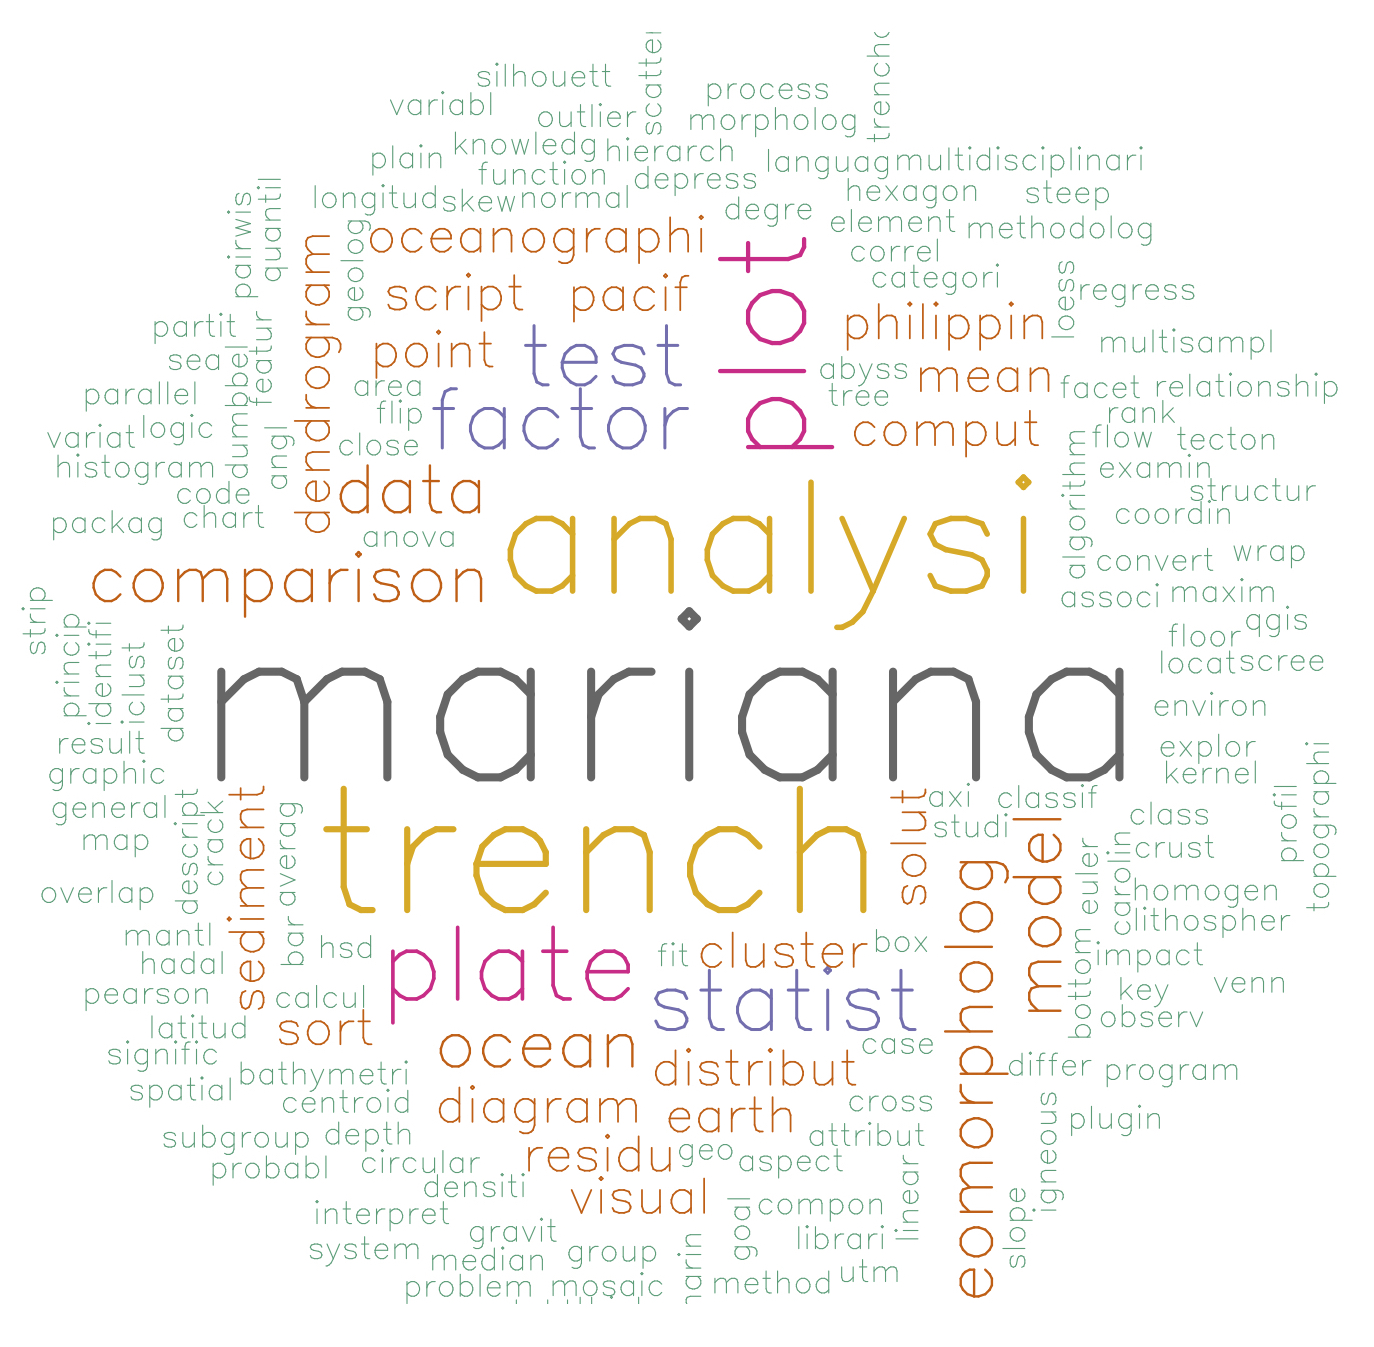
\includegraphics[width=7cm]{Wordcloud.jpg}
\end{figure}		
\end{frame}
 
% ----------------------------------------------------------------------------
% *** END: Final Slide >>>
% ----------------------------------------------------------------------------
\end{document}